\documentclass[a4paper,12pt]{report}
\usepackage[utf8]{inputenc}
\usepackage{listings}
\usepackage[italian]{babel}
\usepackage{geometry}
\geometry{margin=3cm}
\usepackage{titling}
\usepackage{fancyhdr}
\usepackage{enumitem}
\usepackage{braket}
\usepackage{amsmath}
\usepackage{amssymb}
\usepackage{array}
\usepackage{booktabs}
\usepackage{caption}
\usepackage[italicdiff]{physics}
\usepackage{amsthm} % Per ambienti theorem e proof
\usepackage{mathtools}
\usepackage{mathrsfs}
\usepackage{framed}
\usepackage{graphicx}
\usepackage{float} % Forza il posizionamento con [H]
\usepackage{hyperref}
\usepackage{tcolorbox}
\usepackage{varwidth}
\usepackage{booktabs}       % Tabelle professionali
\usepackage{siunitx}        % Formattazione unità


\theoremstyle{plain}
\newtheorem{theorem}{Teorema}[chapter]
\newtheorem{corollario}{Corollario}[chapter]
\newtheorem{definizione}{Definizione}[section]
\newtheorem{teorema}[definizione]{Teorema}
\newtheorem{postulato}{Postulato}[section] 
\fancypagestyle{prima}{
  \fancyhf{}
  \renewcommand{\headrulewidth}{0pt}
  \renewcommand{\footrulewidth}{0pt}
  \fancyfoot[R]{\textbf{Vaccaro Angelo}}
}

\begin{document}

% Prima pagina
\begin{titlepage}
  \thispagestyle{prima}
  \centering
  \vspace*{5cm}
  {\Huge\bfseries Meccanica quantistica per il quantum computing\par}
  \vfill
\end{titlepage}


% Indice
\tableofcontents
\newpage

\chapter{Dalle origini della fisica classica al calcolo quantistico}
\section{Dalla crisi della fisica classica alla nascita della meccanica quantistica}

L'avvento della meccanica quantistica ha radicalmente ridefinito la nostra comprensione della natura, introducendo paradigmi che sfidano l'intuizione classica. Tra le sue implicazioni più rivoluzionarie, emerge il campo della computazione quantistica, un ambito interdisciplinare che unisce fisica, informatica e ingegneria per sfruttare le leggi quantistiche in dispositivi capaci di superare i limiti intrinseci dei calcolatori tradizionali. 
Questa ricerca si propone di esplorare i fondamenti teorici e sperimentali alla base dei computer quantistici, focalizzandosi sul concetto di qubit - l'unità elementare di informazione quantistica - e sulla sua realizzazione attraverso sistemi fisici a due stati. 
Attraverso un'analisi storica, tecnica e concettuale, verranno illustrate le ragioni per cui tali sistemi, quali lo spin elettronico o i livelli energetici atomici, rappresentano non solo un'astrazione matematica, ma il cuore pulsante di algoritmi in grado di risolvere problemi oggi intrattabili, dalla crittografia alla simulazione di materiali complessi. 
Il lavoro si articolerà inoltre nel confronto critico tra modelli classici e quantistici, evidenziando come principi quali la sovrapposizione, l'entanglement e l'indeterminazione ridefiniscano il concetto stesso di "calcolo", aprendo la strada a una nuova era tecnologica.
L'inizio del XX secolo fu segnato da una rivoluzione inattesa nel panorama scientifico, determinata da una serie di crisi emergenti in fisica. 
Le teorie dell'epoca, oggi note come fisica classica, presentavano previsioni incompatibili con i fenomeni osservati, come la cosiddetta "catastrofe ultravioletta", che implicava l'esistenza di energie infinite, o il comportamento degli elettroni, i quali, secondo i modelli tradizionali, avrebbero dovuto spiraleggiare inesorabilmente verso il nucleo atomico. 
In un primo momento, tali problematiche furono affrontate mediante l'introduzione di ipotesi ad hoc all'interno del quadro classico, ma con il progredire della comprensione della struttura atomica e della radiazione, queste soluzioni si rivelarono sempre più complesse e insostenibili. La crisi raggiunse il culmine nei primi anni Venti del Novecento, dopo decenni di dibattiti e sviluppi teorici, conducendo alla formulazione della moderna meccanica quantistica.
Ma cos'è esattamente la meccanica quantistica? Essa costituisce un quadro matematico, o un insieme di regole, che guida la costruzione di teorie fisiche. Un esempio emblematico è l'elettrodinamica quantistica, una teoria che descrive con grande precisione l'interazione tra atomi e luce. Sebbene l'elettrodinamica quantistica sia sviluppata all'interno del contesto della meccanica quantistica, essa include regole specifiche che non sono determinabili esclusivamente attraverso il quadro generale della meccanica quantistica.
La relazione tra la meccanica quantistica e teorie fisiche particolari, come l'elettrodinamica quantistica, è analoga a quella tra il sistema operativo di un computer e il software applicativo: il sistema operativo stabilisce parametri di base e modalità di funzionamento, mentre il software applicativo definisce le modalità di esecuzione di compiti specifici.
Le regole della meccanica quantistica, pur essendo relativamente semplici, risultano controintuitive, anche per gli esperti del settore. I primi rudimenti del calcolo quantistico e dell'informazione quantistica affondano le radici nel desiderio, che da tempo anima i fisici, di comprendere più a fondo la meccanica quantistica. Così come la fisica classica fallì nel descrivere il mondo microscopico, l'informatica classica sta oggi affrontando limiti fisici: la miniaturizzazione dei transistor sta raggiungendo scale atomiche, dove gli effetti quantistici diventano incontrollabili (si veda la \textbf{legge di Moore}, trattata in dettaglio a \textbf{pagina 5}). Questo parallelo storico ha spinto i ricercatori a esplorare un nuovo paradigma: il calcolo quantistico, che sfrutta proprio quelle leggi quantistiche nate per superare le crisi della fisica classica. Il più celebre critico della meccanica quantistica, Albert Einstein, morì senza mai accettare pienamente la teoria alla quale aveva dato un contributo fondamentale. Nel corso di generazioni, i fisici hanno continuato a confrontarsi con la meccanica quantistica, tentando di rendere le sue previsioni più comprensibili.
Uno degli scopi principali del calcolo quantistico e dell'informazione quantistica è sviluppare strumenti che affinchino la nostra comprensione della meccanica quantistica, rendendo le sue previsioni più trasparenti e accessibili alla mente umana. Un importante filone storico che ha contribuito allo sviluppo del calcolo quantistico e dell'informazione quantistica è rappresentato dall'interesse, emerso negli anni '70, volto a ottenere un controllo completo su singoli sistemi quantistici. Prima di tale periodo, le applicazioni della meccanica quantistica riguardavano tipicamente un controllo a livello macroscopico su campioni di massa contenenti un numero estremamente elevato di sistemi quantistici, i quali, tuttavia, non erano direttamente accessibili o manipolabili individualmente. Dagli anni 70 inizia lo sviluppo di numerose tecniche per controllare sistemi quantistici singoli, ma perchè ci fu tutto questo impegno nel raggiungere questo completo controllo sui sistemi? Tralasciando i numerosi aspetti tecnologici e concentrandoci esclusivamente sulla scienza, la risposta principale risiede nel fatto che i ricercatori hanno agito guidati dall'intuizione. 
In effetti, le intuizioni più profonde in ambito scientifico emergono spesso quando si sviluppa un nuovo metodo per esplorare un dominio inesplorato della Natura. Il calcolo quantistico e l'informazione quantistica si inseriscono in modo naturale all'interno di questo programma di ricerca. Questi campi presentano una serie di sfide, che variano per complessità, rivolte a coloro che stanno progettando metodi per manipolare in modo più preciso i singoli sistemi quantistici. 
Inoltre, stimolano lo sviluppo di nuove tecniche sperimentali e offrono indicazioni sulle direzioni più promettenti per l'avanzamento degli esperimenti. Al contempo, la capacità di controllare singoli sistemi quantistici risulta fondamentale per poter sfruttare appieno il potenziale della meccanica quantistica nelle applicazioni relative al calcolo quantistico e all'informazione quantistica. Questo ha portato all'ideazione di possibili sistemi di elaborazione dell'informazione quantistica. 
Fino a poco tempo fa, lo stato dell'arte nel calcolo quantistico era rappresentato da piccoli computer quantistici, in grado di eseguire dozzine di operazioni su pochi quibit (bit quantistici). Negli ultimi anni, ci sono stati significativi avanzamenti nella ricerca sui processori quantistici per una combinazione di fattori tecnologici, scientifici e finanziari. 
Ecco alcuni dei motivi principali dietro questo impulso: 
\begin{itemize}
  \item Miglioramenti nelle tecnologie di fabbricazione dei qubit: Negli ultimi anni, sono stati compiuti progressi nelle tecniche di produzione dei qubit, come quelli basati su superconduttori, trappole ioniche, qubit topologici e persino qubit Majorana. L'ottimizzazione dei metodi di produzione, combinata con una migliore comprensione della fisica dei materiali e delle interazioni quantistiche, ha migliorato la stabilità, la coerenza e la qualità dei qubit.
  \item Avanzamenti nella correzione degli errori quantistici: La correzione degli errori è stata a lungo una delle principali sfide del Quantum Computing, ma negli ultimi anni sono stati fatti importanti passi avanti nel migliorare le tecniche di correzione degli errori quantistici. Nuovi algoritmi e approcci, come la correzione degli errori topologici, hanno il potenziale di ridurre significativamente gli errori nei processori quantistici e migliorare la loro affidabilità.
  \item Miglioramenti nei sistemi di controllo: La precisione nel controllo dei qubit è fondamentale per il funzionamento dei computer quantistici. I recenti progressi nei sistemi di controllo, inclusi i circuiti di feedback avanzati, i laser ultra-precisi e la tecnologia di rilevamento, hanno permesso di ottenere una maggiore precisione nel manipolare i qubit, riducendo gli errori e aumentando la fidelità delle operazioni quantistiche.
  \item Aumento degli investimenti: Negli ultimi anni, c'è stato un enorme aumento degli investimenti nel Quantum Computing, sia da parte di aziende private che di governi. Giganti tecnologici come Google, IBM, Microsoft, Intel e altri, insieme a startup specializzate, stanno investendo miliardi di dollari nella ricerca e nello sviluppo di processori quantistici. Anche i governi di molti paesi (come Stati Uniti, Cina, Unione Europea) hanno stanziato fondi significativi per accelerare i progressi nel campo.
  \item Collaborazioni tra settore pubblico e privato: Le collaborazioni tra università, centri di ricerca e aziende private sono diventate sempre più comuni, creando sinergie che hanno accelerato la ricerca nel Quantum Computing. Queste collaborazioni permettono di combinare l'esperienza accademica con le risorse e l'innovazione del settore privato.
  \item Sviluppo di software quantistico: L'evoluzione del software quantistico, come i linguaggi di programmazione e le librerie per il Quantum Computing, ha stimolato la ricerca hardware. Piattaforme come IBM Qiskit e Google Cirq, ad esempio, permettono ai ricercatori di testare algoritmi quantistici sui computer quantistici, incentivando ulteriori sviluppi nella tecnologia hardware.
  \item Dimostrazione di vantaggi teorici: Alcuni esperimenti recenti hanno mostrato, anche se in modo limitato, vantaggi teorici reali del Quantum Computing rispetto ai computer classici. Questi esperimenti hanno stimolato ulteriormente l'interesse e la fiducia nella possibilità di risolvere problemi che i computer classici non possono affrontare efficacemente, come la simulazione di sistemi molecolari complessi o l'ottimizzazione di grandi quantità di dati.
  \item Progressi nella teoria e nella ricerca fondamentale: Le scoperte teoriche nel campo della fisica quantistica, come nuovi modelli di qubit e metodi per stabilizzare i sistemi quantistici, hanno spinto la ricerca a un livello superiore. Alcuni sviluppi teorici hanno reso possibile progettare qubit più stabili e meno suscettibili agli errori, accelerando la realizzazione di processori quantistici più performanti.
\end{itemize}
Questi fattori, combinati con un crescente interesse globale nel potenziale del Quantum Computing per risolvere problemi complessi in vari campi, come la crittografia, l'ottimizzazione, la simulazione chimica e farmacologica, e il machine learning, hanno portato a un rapido avanzamento nella ricerca e nello sviluppo dei processori quantistici. Sebbene la tecnologia sia ancora nelle sue fasi iniziali, questi sviluppi hanno gettato le basi per futuri progressi significativi nel campo.

\section{Dal modello classico di calcolo al paradigma quantistico}
Ora spostiamo la nostra attenzione dalla meccanica quantistica a un altro dei grandi successi intellettuali del ventesimo secolo: l'informatica. 
Le origini di questa disciplina si perdono nelle profondità della storia. Ad esempio, le tavolette cuneiformi indicano che, al tempo di Hammurabi (circa 1750 a.C.), i Babilonesi avevano già sviluppato concetti algoritmici piuttosto avanzati, e molte di queste idee potrebbero risalire a periodi ancora più remoti. 
L'incarnazione moderna dell'informatica è stata formalizzata dal celebre matematico Alan Turing in un articolo del 1936. Turing elaborò una nozione astratta di quello che oggi definiremmo un computer programmabile, un modello di calcolo ora noto come macchina di Turing, in suo onore. 
Turing dimostrò l'esistenza di una Macchina Universale di Turing, capace di simulare qualsiasi altra macchina di Turing. Inoltre, egli sostenne che questa Macchina Universale di Turing rappresenta completamente ciò che significa eseguire un compito tramite mezzi algoritmici. In altre parole, se un algoritmo può essere eseguito su un dispositivo hardware qualsiasi (come un moderno computer personale), esisterà un algoritmo equivalente per la Macchina Universale di Turing che svolgerà esattamente lo stesso compito dell'algoritmo eseguito sul computer personale. 
Questa affermazione, nota come tesi di Church-Turing, in onore di Turing e dell'altro pioniere dell'informatica Alonzo Church, stabilisce l'equivalenza tra il concetto fisico di quali algoritmi possono essere eseguiti su un dispositivo fisico e il rigoroso concetto matematico della Macchina Universale di Turing. 
L'ampia accettazione di questa tesi ha fornito le basi per lo sviluppo di una teoria solida e approfondita dell'informatica. 
Poco dopo il lavoro di Turing, furono sviluppati i primi computer costruiti con componenti elettronici. John von Neumann propose un modello teorico che descriveva come assemblare in modo pratico tutti i componenti necessari per rendere un computer completamente equivalente a una Macchina Universale di Turing. 
Lo sviluppo dell'hardware dei computer subì una vera e propria accelerazione nel 1947, quando John Bardeen, Walter Brattain e Will Shockley inventarono il transistor. Da quel momento, l'hardware dei computer ha visto un aumento esponenziale della potenza, un fenomeno che fu formalizzato da Gordon Moore nel 1965 con quella che divenne nota come la legge di Moore. 
Questa legge afferma che la potenza di calcolo dei computer raddoppierà a costi costanti ogni circa due anni. Sorprendentemente, la legge di Moore è rimasta valida approssimativamente per i decenni successivi agli anni '60. 
Tuttavia i metodi convenzionali di fabbricazione della tecnologia dei computer stanno cominciando a incontrare ostacoli fondamentali legati alla miniaturizzazione. Gli effetti quantistici iniziano infatti a interferire con il funzionamento dei dispositivi elettronici man mano che vengono realizzati sempre più piccoli. 
Una possibile soluzione al problema derivante dall'eventuale fallimento della legge di Moore consiste nel passare ad un \textbf{paradigma computazionale alternativo}. 
Uno di questi paradigmi è rappresentato dalla teoria del \textbf{calcolo quantistico}, che sfrutta la meccanica quantistica per eseguire calcoli, anziché fare affidamento sulla fisica classica. È stato osservato che, sebbene un computer classico possa simulare un computer quantistico, sembra \textbf{impossibile} farlo in modo efficiente. 
Di conseguenza, i computer quantistici offrono un vantaggio fondamentale in termini di velocità rispetto ai computer classici. Questo vantaggio è talmente significativo che molti ricercatori ritengono che nessun progresso significativo nel campo della computazione classica sarà in grado di colmare il divario di potenza tra un computer classico e uno quantistico. 
Ma cosa si intende per "simulazione efficiente" rispetto a una "simulazione inefficiente" di un computer quantistico? Molti dei concetti chiave necessari per rispondere a questa domanda erano già stati formulati prima che nascesse l'idea di un computer quantistico.
In particolare, il concetto di algoritmi efficienti e inefficienti è stato formalizzato matematicamente dal campo della complessità computazionale. In generale, un algoritmo è considerato efficiente se riesce a completare il calcolo in un tempo \textbf{polinomiale}
\footnote{Un \textbf{tempo polinomiale} significa che il numero di operazioni richieste per risolvere un problema cresce come una potenza (\textbf{polinomio}) della dimensione dell'input. Un algoritmo ha \textbf{complessità polinomiale} se il suo tempo di esecuzione è limitato da una funzione del tipo:
\[
T(n) = O(n^k)
\]
dove:
\begin{itemize}
    \item \( n \) è la dimensione dell'input (ad esempio, il numero di bit necessari per rappresentare un numero);
    \item \( k \) è una costante fissa;
\end{itemize}} 
in relazione alla dimensione del problema da risolvere. Al contrario, un algoritmo inefficiente richiede un tempo \textbf{superpolinomiale}
\footnote{Un algoritmo \textbf{superpolinomiale} è un algoritmo il cui tempo di esecuzione cresce più velocemente di una funzione polinomiale, ma non necessariamente in modo esponenziale. In altre parole, la complessità di un algoritmo superpolinomiale è più alta di quella di un algoritmo polinomiale, ma non raggiunge la rapidità di crescita di un algoritmo esponenziale, non può quindi essere descritto da una funzione del tipo \( O(n^k) \).}, solitamente esponenziale.

\newpage
\noindent Alla fine degli anni '60 e all'inizio degli anni '70, si osservò che il modello di macchina di Turing fosse almeno potente quanto qualsiasi altro modello di computazione, nel senso che un problema risolvibile in modo efficiente in un determinato modello di computazione poteva essere risolto altrettanto efficientemente nel modello della macchina di Turing, utilizzando quest'ultima per simulare l'altro modello. Questa osservazione è stata formalizzata in una versione rafforzata della tesi di Church-Turing, che afferma:
\begin{center}
  \textbf{"Qualsiasi processo algoritmico può essere simulato in modo efficiente utilizzando una macchina di Turing."}
\end{center}
Il rafforzamento principale nella tesi di Church-Turing forte riguarda l'introduzione del concetto di "efficienza". Se la tesi di Church-Turing forte è valida, essa implica che, indipendentemente dal tipo di macchina utilizzata per eseguire un algoritmo, questa macchina può essere simulata in modo efficiente tramite una macchina di Turing standard. Questo è un rafforzamento cruciale, poiché suggerisce che, per valutare se un determinato compito computazionale possa essere eseguito in modo efficiente, è sufficiente concentrarsi sull'analisi del modello della macchina di Turing.
Una delle principali sfide alla tesi di Church-Turing forte proviene dal campo del calcolo analogico. Negli anni successivi alla pubblicazione del lavoro di Turing, diversi gruppi di ricercatori hanno osservato che alcune macchine analogiche erano in grado di risolvere problemi in modo più efficiente rispetto a quanto si pensava fosse possibile su una macchina di Turing. A prima vista, queste macchine sembrano contraddire la forma rafforzata della tesi di Church-Turing. Tuttavia, quando si considerano ipotesi realistiche riguardo alla presenza di rumore nei computer analogici, si scopre che la loro potenza computazionale svanisce nei casi conosciuti, non riuscendo a risolvere problemi che non sono risolvibili in modo efficiente su una macchina di Turing. Questa lezione che \textit{il rumore realistico deve essere preso in considerazione quando si valuta l'efficienza di un modello computazionale} è stata una delle principali difficoltà iniziali nel campo del calcolo quantistico e dell'informazione quantistica. 
Tuttavia, tale difficoltà è stata superata con successo grazie allo sviluppo della teoria dei codici di correzione degli errori quantistici e del calcolo quantistico tollerante agli errori.
Pertanto, a differenza del calcolo analogico, il calcolo quantistico è teoricamente in grado di tollerare una quantità finita di rumore senza compromettere i suoi vantaggi computazionali.
Una delle prime sfide significative alla tesi di Church-Turing forte emerse a metà degli anni '70, quando Robert Solovay e Volker Strassen dimostrarono che è possibile testare la primalità di un numero intero utilizzando un algoritmo randomizzato. 
In altre parole, il test di Solovay-Strassen per la primalità si basa su un elemento di casualità, in quanto l'algoritmo non determina con certezza se un numero intero è primo o composto, ma fornisce una probabilità di correttezza del risultato. In realtà, l'algoritmo di Solovay-Strassen non determinava unicamente se un numero fosse primo o composto con certezza, ma poteva stabilire con alta probabilità che un numero fosse primo o composto. Ripetendo il test più volte, era possibile ottenere una probabilità molto elevata di determinare correttamente la primalità di un numero. 
Il test di Solovay-Strassen rivestiva particolare importanza al momento della sua proposta, poiché all'epoca non esisteva alcun test deterministico per la primalità, e nessuno ne è ancora stato scoperto al momento della scrittura di questo testo. Pertanto, sembrava che i computer con accesso a un generatore di numeri casuali potessero eseguire compiti computazionali che non avevano una soluzione efficiente su una macchina di Turing deterministica convenzionale. Questa scoperta ispirò una ricerca su altri algoritmi randomizzati, che ha dato risultati eccellenti, portando alla nascita di un vivace campo di ricerca. 
Gli algoritmi randomizzati pongono una sfida alla tesi di Church-Turing forte, suggerendo che esistano problemi che possono essere risolti in modo efficiente, ma che non possono essere risolti in modo efficiente da una macchina di Turing deterministica. Questa sfida sembra essere facilmente risolvibile con una semplice modifica della tesi di Church-Turing forte:
\begin{center}
    \textbf{"Qualsiasi processo algoritmico può essere simulato in modo efficiente utilizzando una macchina di Turing probabilistica."}
\end{center}
Nel 1985, David Deutsch si chiese se le leggi della fisica potessero essere utilizzate per derivare una versione più forte della tesi di Church-Turing. Anziché fare ipotesi ad hoc, Deutsch decise di esplorare la teoria fisica per fornire una base solida alla tesi di Church-Turing, così sicura come lo status della teoria fisica stessa. In particolare, Deutsch cercò di definire un dispositivo computazionale capace di simulare in modo efficiente un sistema fisico arbitrario. 
Poiché le leggi della fisica sono intrinsecamente di natura quantistica, Deutsch fu naturalmente indotto a considerare dispositivi computazionali basati sui principi della meccanica quantistica. Questi dispositivi, che rappresentano l'analogo quantistico delle macchine proposte da Turing quasi mezzo secolo prima, portarono alla concezione moderna del computer quantistico. 
Non è ancora chiaro se la nozione di Computer Quantistico Universale proposta da Deutsch sia sufficiente per simulare in modo efficiente un sistema fisico arbitrario. La congettura che questa capacità possa essere raggiunta o meno rimane uno dei grandi problemi aperti nel campo della computazione quantistica e delle informazioni quantistiche. È possibile, infatti, che qualche effetto emergente dalla teoria quantistica dei campi, o un fenomeno più complesso legato alla teoria delle stringhe, alla gravità quantistica o a qualche altra teoria fisica avanzata, possa superare i limiti del modello di Computer Quantistico Universale di Deutsch, proponendo un modello di calcolo ancor più potente. 
Tuttavia, a questo stadio, non vi è certezza al riguardo. Ciò che il modello proposto da Deutsch ha consentito è stato un'importante sfida alla forma forte della tesi di Church-Turing. Deutsch si chiese se un computer quantistico fosse in grado di risolvere in modo efficiente problemi computazionali che non hanno una soluzione efficiente su un computer classico, neppure su una macchina di Turing probabilistica. 
Per illustrare questa possibilità, Deutsch costruì un esempio semplice che suggeriva che i computer quantistici potrebbero possedere capacità computazionali superiori rispetto a quelle dei computer classici, mettendo in discussione le nozioni tradizionali di efficienza computazionale. Il notevole passo iniziale compiuto da Deutsch nel campo della computazione quantistica è stato notevolmente migliorato nel decennio successivo grazie ai contributi di numerosi ricercatori, culminando nella \textbf{fondamentale dimostrazione di Peter Shor nel 1994}. 
Shor dimostrò che due problemi computazionali di importanza cruciale: 
\begin{enumerate}
  \item il problema della fattorizzazione di un intero. \footnote{La fattorizzazione di un numero intero N è il processo di scrivere N come il prodotto di numeri primi.}
  \item il problema del "logaritmo discreto" \footnote{Dato un gruppo \( G \) e un elemento \( g \) di \( G \), il problema del logaritmo discreto consiste nel determinare, per un dato elemento \( y \), l'esponente \( x \) tale che: \[g^x \equiv y \pmod{p}\] dove:
  \begin{itemize}
    \item \( g \) è un generatore del gruppo (cioè un elemento che può generare tutti gli altri elementi del gruppo tramite esponenziazione);
    \item \( p \) è un numero primo che definisce il gruppo (spesso un modulo primo);
    \item \( x \) è l'esponente da determinare (è il logaritmo discreto di \( y \) in base \( g \));
    \item \( y \) è l'elemento del gruppo di cui vogliamo calcolare il logaritmo discreto.
  \end{itemize}
  In altre parole, data l'equazione \( g^x = y \), trovare \( x \) è il problema del logaritmo discreto.}
\end{enumerate}
In altre parole, potevano essere risolti in modo efficiente su un computer quantistico. Questa scoperta suscitò un ampio interesse, poiché tali problemi erano ampiamente considerati insolubili in modo efficiente su un computer classico. 
I risultati di Shor fornirono una forte evidenza del fatto che i computer quantistici possiedano potenzialità computazionali superiori rispetto alle macchine di Turing, incluse quelle probabilistiche. Il quantum computing non è solo una curiosità teorica: algoritmi come quelli di Shor (\textbf{fattorizzazione}) e Grover (\textbf{ricerca non strutturata}) dimostrano vantaggi esponenziali rispetto ai computer classici. 
Questi risultati non sono mere speculazioni, ma hanno implicazioni concrete per la crittografia, l'ottimizzazione e la simulazione di sistemi quantistici. 
Nel 1995, un ulteriore avanzamento nella comprensione delle capacità dei computer quantistici fu fornito da Lov Grover, che dimostrò come un altro problema significativo \textit{la ricerca in uno spazio di ricerca non strutturato} \footnote{La ricerca in uno spazio di ricerca non strutturato è un tipo di problema di ricerca in cui non ci sono informazioni o proprietà specifiche che possono essere utilizzate per ottimizzare il processo di ricerca. In altre parole, lo spazio di ricerca non ha una struttura chiara che possa essere sfruttata per ridurre il numero di passi necessari per trovare una soluzione. Quindi, la ricerca deve avvenire senza avere una guida esplicita su dove trovare la soluzione.} potesse essere accelerato su un computer quantistico. 
Sebbene l'algoritmo di Grover non producesse un'accelerazione spettacolare come quella degli algoritmi di Shor, l'ampia applicabilità delle tecniche basate sulla ricerca ha suscitato un notevole interesse nella comunità scientifica, evidenziando il potenziale pratico dei computer quantistici in contesti computazionali diversi. Le considerazioni teoriche e tecnologiche precedentemente discusse hanno contribuito alla nascita e all'affermarsi di un campo di ricerca oggi noto come teoria dell'informazione e della computazione quantistica. In questo contesto, ci concentreremo in particolare sulle differenze fondamentali tra la computazione quantistica e il paradigma computazionale classico. 
\newpage
\noindent Queste differenze derivano principalmente dai principi della teoria quantistica che governano il comportamento dell'infinitamente piccolo. In particolare, esamineremo tre fenomeni della teoria quantistica, essenziali ma spesso controintuitivi, che costituiscono la base della computazione quantistica e ne determinano il potenziale computazionale straordinario: 
\begin{enumerate}
  \item \textbf{il principio di sovrapposizione degli stati};
  \item \textbf{il principio di misurazione};
  \item \textbf{il fenomeno dell'entanglement};
\end{enumerate}
andando nel profondo dei vari argomenti.

\chapter{Fondamenti di meccanica quantistica}
La meccanica quantistica rappresenta attualmente il quadro teorico più accurato e completo per la descrizione dei fenomeni fisici fondamentali. La sua rilevanza si estende alla computazione quantistica e all'informazione quantistica, discipline le cui basi concettuali derivano interamente dal formalismo quantistico. Questo capitolo fornisce un apparato teorico essenziale per una comprensione rigorosa di tali ambiti, strutturando i principi della meccanica quantistica in modo autoconsistente. Non si presuppone alcuna familiarità pregressa con la teoria.
Contrariamente alla sua percezione diffusa come disciplina di elevata complessità, la meccanica quantistica può essere efficacemente appresa a livello dei suoi fondamenti matematici e concettuali. La reputazione di osticità deriva prevalentemente dalle sfide poste da applicazioni avanzate - \textit{quali la modellizzazione di sistemi molecolari complessi} - le quali non rientrano negli scopi di questa trattazione. L'unico prerequisito richiesto è la conoscenza dell'algebra lineare elementare.

\section{Richiami di algebra lineare}
L'algebra lineare costituisce lo studio assiomatico degli spazi vettoriali e delle trasformazioni lineari agenti su tali strutture. Una comprensione rigorosa della meccanica quantistica necessita di una padronanza consolidata dei suoi principi elementari. In questa sezione si richiamano concetti basilari e si introduce il formalismo notazionale adottato nella trattazione quantistica.
Tale figura articola sistematicamente la notazione quantistica (colonna sinistra) con la descrizione algebrico-lineare canonica (colonna destra).
Gli \textit{spazi vettoriali} rappresentano gli oggetti fondanti della teoria. Di particolare rilevanza è lo spazio \(\mathbb{C}^n\), definito come l'insieme di tutte le \textit{n}-uple ordinate di numeri complessi: \((z_1, \dots, z_n)\), con \(z_k \in \mathbb{C}\). 
Gli elementi di \(\mathbb{C}^n\) sono denominati \textit{vettori} Si adotterà alternativamente la notazione matriciale colonna, allineata alle convenzioni della letteratura quantistica:
\[
\begin{bmatrix}
  z_1 \\
  \vdots \\
  z_n
\end{bmatrix}
\]
Sullo spazio è definita un'operazione binaria di \textbf{addizione vettoriale} che porta coppie di vettori ad altri vetttori. In \(\mathbb{C}^n\) l'operazione di addizione per i vettori è definita da:
\[
\begin{bmatrix} 
z_1 \\ 
\vdots \\ 
z_n 
\end{bmatrix} 
+ 
\begin{bmatrix} 
z_1' \\ 
\vdots \\ 
z_n' 
\end{bmatrix} 
\equiv 
\begin{bmatrix} 
z_1 + z_1' \\ 
\vdots \\ 
z_n + z_n' 
\end{bmatrix},
\]
dove le operazioni di addizione a destra sono ordinarie addizioni di numeri complessi. Inoltre, in uno spazio vettoriale è presente un'operazione di \textbf{moltiplicazione per uno scalare}. In \(\mathbb{C}^n\) questa operazione è definita da:
\[
z \, 
\begin{bmatrix} 
    z_1     \\ 
    \vdots  \\ 
    z_n 
\end{bmatrix} 
\equiv
\begin{bmatrix} 
    z z_1   \\ 
    \vdots  \\ 
    z z_n 
\end{bmatrix},
\]
dove \textit{z} è uno \textbf{scalare}, cioè un numero complesso, e le moltiplicazioni a destra sono \textbf{moltiplicazioni ordinarie di numeri complessi}. I fisici talvolta si riferiscono ai numeri complessi come \textit{c-numeri}. Essendo un testo in cui trattiamo la meccanica quantistica utilizzeremo la \textbf{notazione standard della meccanica quantistica} per i concetti algebrico-lineare.
Lo notazione standard della meccanica quantistica per un vettore in uno spazio vettoriale è il seguente: 
\[
\ket{\psi}.
\]
Nell'algebra lineare quantistica, un vettore è indicato con un'etichetta arbitraria (tipicamente lettere greche come $\psi$ o $\phi$) racchiusa nella \textbf{notazione braket}:
\[
|\ket{\psi}
\]
dove:
\begin{itemize}
    \item $\psi$ è un identificatore arbitrario (qualsiasi simbolo è ammissibile);
    \item La sintassi \(\ket{\cdot}\) specifica che l'oggetto è un vettore;
    \item Il simbolo completo \(\ket{\psi}\) è denominato \textit{ket} (terminologia usata raramente nel nostro contesto).
\end{itemize}
Ogni spazio vettoriale possiede un elemento speciale chiamato \textbf{vettore zero}, che indichiamo con il simbolo $\mathbf{0}$. Questo vettore ha una proprietà unica: sommato a qualsiasi altro vettore $|\mathbf{v}\rangle$ lascia quest'ultimo invariato:
\[
|\mathbf{v}\rangle + \mathbf{0} = |\mathbf{v}\rangle
\]
\begin{itemize}
  \item \textbf{Non usiamo mai} la notazione ket per il vettore zero: $\mathbf{0} \neq |0\rangle$;
  \item Questa è l'\textbf{unica eccezione} alla regola della notazione ket;
  \item Perché? Per evitare confusione: $|0\rangle$ in meccanica quantistica indica uno \textbf{stato fondamentale}, completamente diverso dal vettore nullo.
\end{itemize}
Quando moltiplichiamo il vettore zero per un qualsiasi numero complesso $z \in \mathbb{C}$, otteniamo sempre il vettore zero:
\[
z \cdot \mathbf{0} = \mathbf{0}
\]
In $\mathbb{C}^n$ (spazio delle n-uple complesse):
\begin{itemize}
  \item Usiamo la notazione $(z_1, \dots, z_n)$ per le matrici colonna
  \item Il vettore zero si rappresenta come:
\[
(0, 0, \dots, 0)
\]
  \item Esempio in $\mathbb{C}^2$: $\mathbf{0} = (0, 0)$
\end{itemize}
Un \textbf{sottospazio vettoriale} $W$ di uno spazio $V$ è un sottoinsieme che soddisfa due condizioni essenziali:

\begin{enumerate}
  \item \textbf{Chiusura rispetto alla moltiplicazione scalare}:
\[
\text{Se } |\mathbf{w}\rangle \in W \text{ allora } z \cdot |\mathbf{w}\rangle \in W \quad \forall z \in \mathbb{C}
\]

  \item \textbf{Chiusura rispetto all'addizione}:
\[
\text{Se } |\mathbf{w}_1\rangle, |\mathbf{w}_2\rangle \in W \text{ allora } |\mathbf{w}_1\rangle + |\mathbf{w}_2\rangle \in W
\]
\end{enumerate}
\begin{itemize}
  \item In $\mathbb{R}^2$, esempi di sottospazi sono:
\begin{itemize}
  \item L'origine: $\{\mathbf{0}\}$
  \item Una retta passante per l'origine
  \item L'intero piano
\end{itemize}
  \item \textbf{Non} sono sottospazi: rette non passanti per l'origine, figure e curve.
\end{itemize}
\newpage
\begin{table}[h]
\centering
\caption{Riassunto di alcune notazioni standard della meccanica quantistica per nozioni di algebra lineare. Questo stile di notazione è noto come notazione di \emph{Dirac}.}
\label{tab:dirac-notation}
\begin{tabular}{|>{$}c<{$}|p{0.7\textwidth}|}
\hline
\textbf{Notazione} & \textbf{Descrizione} \\
\hline
z^* & Coniugato complesso del numero complesso \( z \). Esempio: \((1 + i)^* = 1 - i\) \\
\hline
|\psi\rangle & Vettore. Noto anche come \emph{ket}. \\
\hline
\langle\psi| & Vettore duale a \(|\psi\rangle\). Noto anche come \emph{bra}. \\
\hline
\langle\varphi|\psi\rangle & Prodotto scalare tra i vettori \(|\varphi\rangle\) e \(|\psi\rangle\). \\
\hline
|\varphi\rangle \otimes |\psi\rangle & Prodotto tensoriale di \(|\varphi\rangle\) e \(|\psi\rangle\). \\
\hline
|\varphi\rangle|\psi\rangle & Notazione abbreviata per il prodotto tensoriale di \(|\varphi\rangle\) e \(|\psi\rangle\). \\
\hline
A^* & Coniugato complesso della matrice \(A\). \\
\hline
A^T & Trasposta della matrice \(A\). \\
\hline
A^{\dagger} & Coniugato hermitiano o aggiunto della matrice \(A\), dove \(A^{\dagger} = (A^T)^*\). \\
& Esempio: 
\[\begin{bmatrix} a & b \\ c & d \end{bmatrix}^{\dagger} = \begin{bmatrix} a^* & c^* \\ b^* & d^* \end{bmatrix}\] \\
\hline
\langle\varphi|A|\psi\rangle & Prodotto scalare tra \(|\varphi\rangle\) e \(A|\psi\rangle\). \\
& Equivalentemente, prodotto scalare tra \(A^{\dagger}|\varphi\rangle\) e \(|\psi\rangle\). \\
\hline
\end{tabular}
\end{table}

\subsection{Basi e indipendenza lineare}
Un insieme generatore (o spanning set) per uno spazio vettoriale è un insieme di vettori \(|v_1\rangle, \ldots, |v_n\rangle\) tale che ogni vettore \(|v\rangle\) appartenente allo spazio può essere scritto come combinazione lineare dei vettori dell'insieme, ovvero:

\[|v\rangle = \sum_i a_i |v_i\rangle,\]

\noindent dove gli \(a_i\) sono coefficienti (in generale complessi).

Ad esempio, l'insieme

\[|v_1\rangle = 
\begin{bmatrix}
1 \\
0
\end{bmatrix},
\quad |v_2\rangle = 
\begin{bmatrix}
0 \\
1
\end{bmatrix}\]

è un insieme generatore per lo spazio vettoriale \(\mathbb{C}^2\), poiché qualsiasi vettore

\[|v\rangle = 
\begin{bmatrix}
a_1 \\
a_2
\end{bmatrix}\]

può essere espresso come

\[|v\rangle = a_1 |v_1\rangle + a_2 |v_2\rangle.\]
In questo caso, diciamo che \(|v_1\rangle\) e \(|v_2\rangle\) generano lo spazio \(\mathbb{C}^2\). In generale, uno spazio vettoriale può ammettere diversi insiemi generatori. Un altro esempio per \(\mathbb{C}^2\) è:

\[|v_1\rangle = \frac{1}{\sqrt{2}} 
\begin{bmatrix}
1 \\
1
\end{bmatrix},
\quad |v_2\rangle = \frac{1}{\sqrt{2}} 
\begin{bmatrix}
1 \\
-1
\end{bmatrix}.\]

\noindent Anche in questo caso, un qualunque vettore \(|v\rangle = 
\begin{bmatrix}
a_1 \\
a_2
\end{bmatrix}\) può essere riscritto come combinazione lineare dei due vettori precedenti:

\[|v\rangle = \frac{a_1 + a_2}{\sqrt{2}} |v_1\rangle + \frac{a_1 - a_2}{\sqrt{2}} |v_2\rangle.\]
Un concetto fondamentale legato agli insiemi generatori è quello di dipendenza lineare.
Un insieme di vettori \(|v_1\rangle, \ldots, |v_n\rangle\) è detto \emph{linearmente dipendente} se esistono coefficienti \(a_1, \ldots, a_n\), non tutti nulli, tali che:

\[a_1|v_1\rangle + a_2|v_2\rangle + \cdots + a_n|v_n\rangle = 0.\]
In caso contrario, l'insieme si dice \emph{linearmente indipendente}.
Un insieme di vettori che sia \textbf{linearmente indipendente} e \textbf{generi} lo spazio vettoriale viene detto base dello spazio. È possibile dimostrare che tutte le basi di uno stesso spazio vettoriale hanno lo stesso numero di vettori. Questo numero prende il nome di dimensione dello spazio vettoriale.
Nel contesto di questa trattazione, ci concentreremo esclusivamente su \textbf{spazi vettoriali di dimensione finita}. Sebbene gli spazi di dimensione infinita offrano molti spunti di studio teoricamente interessanti, spesso anche complessi, essi esulano dagli obiettivi di questo lavoro.

\subsection{Operatori lineari e matrici}
Un operatore lineare tra due spazi vettoriali \( V \) e \( W \) è una funzione \( A : V \to W \) che soddisfa la linearità, ovvero per ogni insieme di vettori \(\{|v_i\rangle\} \subseteq V\) e coefficienti complessi \(\{a_i\} \subseteq \mathbb{C}\), vale la seguente relazione:
\[A \left( \sum_i a_i |v_i\rangle \right) = \sum_i a_i A(|v_i\rangle).\]
Nel seguito, adotteremo la notazione compatta \( A|v\rangle \) in luogo di \( A(|v\rangle) \), ove non vi siano ambiguità. Quando si afferma che un operatore lineare \( A \) è definito su uno spazio vettoriale \( V \), si intende che esso è un'applicazione lineare da \( V \) in sé, cioè \( A : V \to V \).
Un esempio fondamentale di operatore lineare è l'operatore identità \( I_V \), definito da:
\[I_V |v\rangle \equiv |v\rangle \quad \text{per ogni } |v\rangle \in V.\]
Quando il contesto è chiaro, ometteremo il pedice e scriveremo semplicemente \( I \). Un altro operatore rilevante è l'operatore nullo, denotato con \( 0 \), che associa a ogni vettore di \( V \) il vettore nullo: \( 0|v\rangle = 0 \) per ogni \( |v\rangle \in V \).
Come è evidente dalla linearità, l'azione di un operatore lineare è completamente determinata dalla sua azione su una base dello spazio vettoriale: se si conosce \( A|v_i\rangle \) per ogni vettore di base \( |v_i\rangle \), allora \( A|v\rangle \) è determinato per ogni \( |v\rangle \in V \).
Siano ora \( V, W \) e \( X \) tre spazi vettoriali, e siano \( A : V \to W \) e \( B : W \to X \) due operatori lineari. La composizione \( BA \) è definita da:
\[(BA)(|v\rangle) \equiv B(A(|v\rangle)),\]
e si scrive semplicemente \( BA|v\rangle \), omettendo le parentesi, secondo l'uso standard.
Il modo più pratico per rappresentare e comprendere gli operatori lineari consiste nell'utilizzare le loro rappresentazioni matriciali. In effetti, esiste una corrispondenza biunivoca tra operatori lineari e matrici, e la teoria delle matrici può essere vista come un caso particolare della teoria degli operatori.
Una matrice complessa \( A \in \mathbb{C}^{m \times n} \), con elementi \( A_{ij} \), definisce un operatore lineare da \( \mathbb{C}^n \) a \( \mathbb{C}^m \), mediante la usuale moltiplicazione matrice-vettore. La condizione di linearità si traduce nel fatto che, per ogni combinazione lineare \( \sum_i a_i |v_i\rangle \), vale:
\[A \left( \sum_i a_i |v_i\rangle \right) = \sum_i a_i A |v_i\rangle,\]
dove \( A |v_i\rangle \) è ottenuto moltiplicando la matrice \( A \) per il vettore colonna \( |v_i\rangle \). Questo mostra chiaramente che ogni matrice definisce un operatore lineare.
Viceversa, è sempre possibile rappresentare un operatore lineare tramite una matrice. Sia \( A : V \rightarrow W \) un operatore lineare tra due spazi vettoriali complessi di dimensione finita. Fissate due basi, rispettivamente \( \{|v_1\rangle, \ldots, |v_m\rangle\} \) per \( V \), e \( \{|w_1\rangle, \ldots, |w_n\rangle\} \) per \( W \), l'azione dell'operatore \( A \) su ciascun vettore di base \( |v_j\rangle \) può essere scritta come:
\[A |v_j\rangle = \sum_i A_{ij} |w_i\rangle.\]
I coefficienti \( A_{ij} \in \mathbb{C} \) costituiscono la matrice rappresentativa dell'operatore \( A \) rispetto alle basi scelte. Questa rappresentazione matriciale è equivalente all'operatore astratto: ogni operatore lineare può essere rappresentato da una matrice, e viceversa, ogni matrice definisce un operatore lineare una volta fissate le basi.
Per costruire tale rappresentazione, è quindi essenziale specificare esplicitamente una base per lo spazio di partenza e una base per lo spazio di arrivo.

\subsection{Matrici di Pauli}
Quattro matrici estremamente utili che avremo spesso occasione di usare sono le \textit{matrici di Pauli}. Queste sono matrici $2 \times 2$, che vengono indicate con una varietà di notazioni. Le matrici, e le loro notazioni corrispondenti, sono illustrate nella Figura 2.2. Le matrici di Pauli sono così utili nello studio del calcolo quantistico e dell'informazione quantistica che vi incoraggiamo a memorizzarle lavorando in dettaglio attraverso i molti esempi ed esercizi basati su di esse nelle sezioni successive.
$$ \sigma_0 \equiv I \equiv \begin{bmatrix} 1 & 0 \\ 0 & 1 \end{bmatrix} \qquad \sigma_1 \equiv \sigma_x \equiv X \equiv \begin{bmatrix} 0 & 1 \\ 1 & 0 \end{bmatrix} $$
$$ \sigma_2 \equiv \sigma_y \equiv Y \equiv \begin{bmatrix} 0 & -i \\ i & 0 \end{bmatrix} \qquad \sigma_3 \equiv \sigma_z \equiv Z \equiv \begin{bmatrix} 1 & 0 \\ 0 & -1 \end{bmatrix} $$
Figura 2.2. Le matrici di Pauli. A volte $I$ è omessa dalla lista, con solo $X, Y$ e $Z$ note come matrici di Pauli.

\subsection{Prodotti interni}
Un prodotto interno su uno spazio vettoriale complesso \( V \) è una funzione  
\[(\cdot, \cdot) : V \times V \rightarrow \mathbb{C}\]  
che associa a ogni coppia di vettori \( \ket{v}, \ket{w} \in V \) un numero complesso \(\braket{v|w} \in \mathbb{C}\), e che soddisfa le seguenti proprietà fondamentali:  
\begin{enumerate}
    \item \textbf{Linearità nel secondo argomento:}  
        Per ogni \( \ket{v} \in V \) e per ogni combinazione lineare \(\sum_i \lambda_i \ket{w_i} \in V\), con \(\lambda_i \in \mathbb{C}\), vale:  
        \[
        \bra{v} \left( \sum_i \lambda_i \ket{w_i} \right) = \sum_i \lambda_i \braket{v|w_i}.
        \]    
    \item \textbf{Coniugazione nel primo argomento (coniugato hermitiano):}  
        Per ogni \( \ket{v}, \ket{w} \in V \), si ha:  
        \[
        \braket{v|w} = \braket{w|v}^*.
        \]
    \item \textbf{Positività definita:}  
        Per ogni \( \ket{v} \in V \), si ha:  
        \[
        \braket{v|v} \geq 0,
        \]  
        con  
        \[
        \braket{v|v} = 0 \iff \ket{v} = 0.
        \]
\end{enumerate}
Lo spazio vettoriale \( V \), insieme a un prodotto interno che soddisfa le proprietà sopra elencate, è detto spazio con prodotto interno.
Nel caso dello spazio vettoriale \( \mathbb{C}^n \), il prodotto interno standard tra due vettori
\[
\mathbf{y} = (y_1, \ldots, y_n), \quad \mathbf{z} = (z_1, \ldots, z_n) \in \mathbb{C}^n
\]
è definito da:
\[
(\mathbf{y}, \mathbf{z}) = \sum_{i=1}^n y_i^* z_i = 
\begin{bmatrix} y_1^* & \cdots & y_n^* \end{bmatrix} 
\begin{bmatrix} z_1 \\ \vdots \\ z_n \end{bmatrix}.
\]
Nel contesto della meccanica quantistica, è consuetudine utilizzare la \textbf{notazione di Dirac}, detta \textbf{notazione bra-ket}, per esprimere il prodotto interno. Dato un vettore \( \ket{v} \in V \), si associa al suo \textbf{vettore duale (o bra)}  
\( \bra{v} \in V^* \), un funzionale lineare definito da:
\[
\bra{v} : V \rightarrow \mathbb{C}, \quad \text{tale che} \quad \bra{v}\ket{w} \equiv \braket{v|w}.
\]
In termini matriciali, se \( \ket{v} \) è rappresentato da un vettore colonna, allora \( \bra{v} \) è il suo complesso coniugato trasposto, ovvero un vettore riga:
\[
\bra{v} = (\ket{v})^\dagger.
\]
\fbox{\begin{minipage}{0.95\textwidth}
\textbf{Box 2.1: La disuguaglianza di Cauchy-Schwarz}
La disuguaglianza di Cauchy-Schwarz è un importante fatto geometrico sugli spazi di Hilbert. Afferma che per due vettori qualsiasi $\ket{v}$ e $\ket{w}$, $|\braket{v|w}|^2 \le \braket{v|v} \braket{w|w}$. Per vederlo, si usi il procedimento di Gram-Schmidt per costruire una base ortonormale $\{\ket{i}\}$ per lo spazio vettoriale tale che il primo vettore della base $\ket{i}$ sia $\ket{w}/\sqrt{\braket{w|w}}$. Usando la relazione di completezza $\sum_i \ket{i}\bra{i} = I$, ed eliminando alcuni termini non negativi si ottiene:
\begin{align*}
\braket{v|v} \braket{w|w} &= \sum_i \braket{v|i} \braket{i|v} \braket{w|w} \\
&\ge \frac{\braket{v|w} \braket{w|v}}{\braket{w|w}} \cdot \braket{w|w} \\
&= \braket{v|w} \braket{w|v} = |\braket{v|w}|^2,
\end{align*}
come richiesto. Un breve ragionamento mostra che l'uguaglianza si verifica se e solo se $\ket{v}$ e $\ket{w}$ sono linearmente dipendenti, $\ket{v} = z\ket{w}$ o $\ket{w} = z\ket{v}$, per qualche scalare $z$.
\end{minipage}}

\subsection{Autovettori ed autovalori}
Sia \( A \) un operatore lineare su uno spazio vettoriale \( V \) sul campo \( \mathbb{C} \). Un vettore non nullo \( \ket{v} \in V \) si dice \textbf{autovettore} di \( A \) se esiste un numero complesso \( \lambda \in \mathbb{C} \), detto \textbf{autovalore}, tale che:
\[
A\ket{v} = \lambda\ket{v}.
\]
L'autovalore \( \lambda \) è associato all'autovettore \( \ket{v} \), e la coppia \( (\lambda, \ket{v}) \) caratterizza una direzione nello spazio \( V \) che è invariata per azione di \( A \), se non per un fattore di scala.
Per semplicità, nel prosieguo adotteremo la convenzione, comune nella letteratura fisica, di utilizzare la stessa notazione \( v \) sia per indicare un autovalore che come etichetta dell'autovettore corrispondente \( \ket{v} \), ove il contesto renda chiaro il significato.
Per determinare gli autovalori di \( A \), si considera l'equazione caratteristica, definita dalla condizione:
\[
\det(A - \lambda I) = 0,
\]
dove \( I \) è l'operatore identità su \( V \). La funzione
\[
c(\lambda) := \det(A - \lambda I),
\]
detta funzione caratteristica di \( A \), è un polinomio in \( \lambda \) i cui zeri individuano gli autovalori di \( A \). Sebbene la funzione caratteristica venga calcolata a partire da una rappresentazione matriciale di \( A \), essa è invariante rispetto alla base scelta, e dipende unicamente dall'operatore stesso.
Per il Teorema Fondamentale dell'Algebra, ogni polinomio non costante a coefficienti complessi ammette almeno una radice in \( \mathbb{C} \). Ne consegue che ogni operatore lineare \( A \) su uno spazio vettoriale complesso ammette almeno un autovalore, e quindi almeno un autovettore non nullo.
Dato un autovalore \( \lambda \) di \( A \), l'insieme
\[
E_{\lambda} := \{\ket{v} \in V \mid A\ket{v} = \lambda\ket{v}\}
\]
è detto \textbf{autospazio} corrispondente a \( \lambda \). Esso costituisce un sottospazio vettoriale di \( V \), ed è non banale per definizione di autovalore.
Un operatore \( A \) si dice diagonalizzabile se ammette una base ortonormale di autovettori \(\{\ket{i}\}\) rispetto alla quale può essere scritto nella forma:
\[
A = \sum_i \lambda_i \ket{i}\bra{i},
\]
dove \(\lambda_i\) sono gli autovalori corrispondenti. Tale espressione è detta rappresentazione diagonale di \(A\), ed è anche nota come decomposizione spettrale o decomposizione ortonormale dell'operatore.
Un esempio rilevante in ambito quantistico è dato dalla matrice di Pauli \(Z\), definita da:
\[
Z = 
\begin{bmatrix}
1 & 0 \\
0 & -1
\end{bmatrix}.
\]
Questa può essere espressa nella forma diagonale:
\[
Z = \ket{0}\bra{0} - \ket{1}\bra{1},
\]
dove \( \ket{0} = \begin{bmatrix} 1 \\ 0 \end{bmatrix} \) e \( \ket{1} = \begin{bmatrix} 0 \\ 1 \end{bmatrix} \), formano una base ortonormale di autovettori.
Si dice che un autovalore \(\lambda\) è \textbf{degenere} se il relativo autospazio \(E_\lambda\) ha dimensione strettamente maggiore di uno. In tal caso, esistono più autovettori linearmente indipendenti associati al medesimo autovalore. Un esempio di degenerazione è fornito dalla matrice:
\[
A = 
\begin{bmatrix}
2 & 0 & 0 \\
0 & 2 & 0 \\
0 & 0 & 0
\end{bmatrix},
\]
la quale ammette un autospazio di dimensione due corrispondente all'autovalore \(\lambda = 2\). I vettori
\[
\begin{bmatrix} 1 \\ 0 \\ 0 \end{bmatrix} \quad \text{e} \quad \begin{bmatrix} 0 \\ 1 \\ 0 \end{bmatrix}
\]
sono esempi di autovettori degeneri, in quanto linearmente indipendenti e associati al medesimo autovalore.

\subsection{Operatori aggiunti ed Hermitiani}
Supponiamo che $A$ sia un qualsiasi operatore lineare su uno spazio di Hilbert, $V$. Si scopre che esiste un unico operatore lineare $A^\dagger$ su $V$ tale che per tutti i vettori $\ket{v}, \ket{w} \in V$,
\begin{align*}
(\bra{v}, A\ket{w}) = (\bra{A^\dagger v}, \ket{w}).
\end{align*}
Questo operatore lineare è noto come \textbf{aggiunto} o \textbf{coniugato hermitiano} dell'operatore $A$. Dalla definizione è facile vedere che $(AB)^\dagger = B^\dagger A^\dagger$. Per convenzione, se $\ket{v}$ è un vettore, allora definiamo $\ket{v}^\dagger \equiv \bra{v}$. Con questa definizione non è difficile vedere che $(A\ket{v})^\dagger = \bra{v}A^\dagger$.

\fbox{\parbox{\dimexpr\linewidth-2\fboxsep-2\fboxrule}{
\textbf{Riquadro 2.2: La decomposizione spettrale -- importante!}
La \emph{decomposizione spettrale} è un teorema di rappresentazione estremamente utile per operatori normali.
\begin{theorem}[2.1]
(Decomposizione spettrale) Qualunque operatore normale $M$ su uno spazio vettoriale $V$ è diagonale rispetto a qualche base ortonormale per $V$. Viceversa, qualunque operatore diagonalizzabile è normale.
\end{theorem}
\begin{proof}
Il viceversa è un semplice esercizio, quindi dimostriamo soltanto l'implicazione diretta per induzione sulla dimensione $d$ di $V$. Il caso $d = 1$ è banale. Sia $\lambda$ un autovalore di $M$, $P$ il proiettore sull'autospazio di $\lambda$, e $Q$ il proiettore sul complemento ortogonale. Allora $M = (P + Q)M(P + Q) = PMP + QMP + PMQ + QMQ$. Ovviamente $PMP = \lambda P$. Inoltre, $QMP = 0$, poiché $M$ mappa il sottospazio $P$ in sé stesso. Affermiamo che anche $PMQ = 0$. Per vederlo, sia $|v\rangle$ un elemento del sottospazio $P$. Allora $MM^{\dagger}|v\rangle = M^{\dagger}M|v\rangle = \lambda M^{\dagger}|v\rangle$. Dunque $M^{\dagger}|v\rangle$ ha autovalore $\lambda$ e pertanto è un elemento del sottospazio $P$. Ne segue che $QM^{\dagger}P = 0$. Prendendo l'aggiunto di questa equazione si ottiene $PMQ = 0$. Quindi $M = PMP + QMQ$. Successivamente, dimostriamo che $QMQ$ è normale. Per vederlo, notiamo che $QM = QM(P + Q) = QMQ$, e $QM^{\dagger} = QM^{\dagger}(P + Q) = QM^{\dagger}Q$. Pertanto, per la normalità di $M$, e l'osservazione che $Q^2 = Q$,
\begin{align*}
QMQQM^{\dagger}Q &= QMQM^{\dagger}Q \\
&= QMM^{\dagger}Q \\
&= QM^{\dagger}MQ \\
&= QM^{\dagger}QMQ \\
&= QM^{\dagger}QQMQ,
\end{align*}
quindi $QMQ$ è normale. Per induzione, $QMQ$ è diagonale rispetto a qualche base ortonormale per il sottospazio $Q$, e $PMP$ è già diagonale rispetto a qualche base ortonormale per $P$. Ne segue che $M = PMP + QMQ$ è diagonale rispetto a qualche base ortonormale per l'intero spazio vettoriale.
\end{proof}
In termini di rappresentazione con prodotto esterno, ciò significa che $M$ può essere scritto come $M = \sum_i \lambda_i |i\rangle\langle i|$, dove $\lambda_i$ sono gli autovalori di $M$, $\{|i\rangle\}$ è una base ortonormale per $V$, e ciascun $|i\rangle$ è un autovettore di $M$ con autovalore $\lambda_i$. In termini di proiettori, $M = \sum_i \lambda_i P_i$, dove $\lambda_i$ sono nuovamente gli autovalori di $M$, e $P_i$ è il proiettore sull'autospazio di $\lambda_i$ di $M$. Questi proiettori soddisfano la relazione di completezza $\sum_i P_i = I$, e la relazione di ortonormalità $P_i P_j = \delta_{ij} P_i$.
}}

\subsection{Prodotto tensoriale}
Il prodotto tensoriale costituisce un'operazione fondamentale nella costruzione di spazi vettoriali di dimensione superiore a partire da spazi vettoriali dati. Tale costruzione riveste un ruolo centrale nella formulazione della meccanica quantistica dei sistemi composti, ovvero quelli costituiti da più sottosistemi. In questa sezione si fornisce una trattazione formale del prodotto tensoriale tra spazi di Hilbert e dei principali oggetti matematici associati.
Siano $V$ e $W$ due spazi di Hilbert complessi di dimensione finita $m$ e $n$, rispettivamente. Si definisce il loro prodotto tensoriale $V \otimes W$ come lo spazio vettoriale di dimensione $mn$, generato formalmente da tutte le combinazioni lineari di elementi del tipo $|v\rangle \otimes |w\rangle$, con $|v\rangle \in V$ e $|w\rangle \in W$. Gli elementi del prodotto tensoriale $V \otimes W$ sono dunque vettori del tipo
$$ |\psi\rangle = \sum_{i,j} c_{ij} |v_i\rangle \otimes |w_j\rangle, $$
dove $\{|v_i\rangle\}$ e $\{|w_j\rangle\}$ sono basi ortonormali per $V$ e $W$, rispettivamente, e $c_{ij} \in \mathbb{C}$. In letteratura, per semplificare la notazione, è comune omettere il simbolo esplicito del prodotto tensoriale, utilizzando invece scritture come $|v\rangle|w\rangle$, $|v, w\rangle$ o $|vw\rangle$.
A livello algebrico, il prodotto tensoriale soddisfa le seguenti proprietà fondamentali:
\begin{enumerate}
    \item \textbf{Compatibilità con la moltiplicazione scalare:}
    $$ z(|v\rangle \otimes |w\rangle) = (z|v\rangle) \otimes |w\rangle = |v\rangle \otimes (z|w\rangle), \quad \forall z \in \mathbb{C}. $$
    \item \textbf{Distributività a sinistra:}
    $$ (|v_1\rangle + |v_2\rangle) \otimes |w\rangle = |v_1\rangle \otimes |w\rangle + |v_2\rangle \otimes |w\rangle. $$
    \item \textbf{Distributività a destra:}
    $$ |v\rangle \otimes (|w_1\rangle + |w_2\rangle) = |v\rangle \otimes |w_1\rangle + |v\rangle \otimes |w_2\rangle. $$
\end{enumerate}
Sia ora $A : V \to V$ un operatore lineare su $V$, e $B : W \to W$ un operatore lineare su $W$. Si definisce il prodotto tensoriale degli operatori $A$ e $B$, denotato con $A \otimes B$, come l'operatore lineare su $V \otimes W$ tale che
$$ (A \otimes B) (|v\rangle \otimes |w\rangle) = (A|v\rangle) \otimes (B|w\rangle), $$
per ogni $|v\rangle \in V, |w\rangle \in W$. Tale definizione si estende per linearità a tutto lo spazio $V \otimes W$, ovvero
$$ (A \otimes B) \left( \sum_i a_i |v_i\rangle \otimes |w_i\rangle \right) = \sum_i a_i (A|v_i\rangle) \otimes (B|w_i\rangle). $$
Questa costruzione può essere generalizzata al caso in cui $A : V \to V'$ e $B : W \to W'$, con $V'$ e $W'$ spazi vettoriali (o spazi di Hilbert) arbitrari. In tal caso, si definisce un operatore $C : V \otimes W \to V' \otimes W'$ come combinazione lineare di prodotti tensoriali di operatori:
$$ C = \sum_i c_i A_i \otimes B_i, $$
dove ciascun $A_i : V \to V'$, $B_i : W \to W'$, e $c_i \in \mathbb{C}$. L'azione di tale operatore su vettori del tipo $|v\rangle \otimes |w\rangle$ è data da
$$ C(|v\rangle \otimes |w\rangle) = \sum_i c_i A_i |v\rangle \otimes B_i |w\rangle. $$
Poiché $V$ e $W$ sono spazi di Hilbert, si può naturalmente definire un \textbf{prodotto interno} su $V \otimes W$ a partire dai prodotti interni definiti su $V$ e $W$. Dati due vettori generici
$$ |\psi\rangle = \sum_i a_i |v_i\rangle \otimes |w_i\rangle, \quad |\phi\rangle = \sum_j b_j |v'_j\rangle \otimes |w'_j\rangle, $$
si definisce
$$ \langle\psi|\phi\rangle := \sum_{i,j} a_i^* b_j \langle v_i|v'_j\rangle \langle w_i|w'_j\rangle. $$
Si può dimostrare che tale funzione soddisfa le proprietà di un prodotto interno, rendendo $V \otimes W$ uno spazio di Hilbert. Di conseguenza, lo spazio tensoriale eredita le nozioni standard associate a strutture di Hilbert, quali gli operatori aggiunti, le trasformazioni unitarie, gli operatori normali e gli operatori hermitiani.
La trattazione precedente ha introdotto il concetto di prodotto tensoriale in termini generali. Tuttavia, per applicazioni pratiche e computazionali risulta utile ricorrere a una rappresentazione matriciale esplicita, nota come \textbf{prodotto di Kronecker}.
Siano \( A \in \mathbb{C}^{m \times n} \) e \( B \in \mathbb{C}^{p \times q} \) due matrici. Il loro \textbf{prodotto di Kronecker} è definito come la matrice \( A \otimes B \in \mathbb{C}^{mp \times nq} \) data da:
\[
A \otimes B = 
\begin{pmatrix}
A_{11}B & A_{12}B & \cdots & A_{1n}B \\
A_{21}B & A_{22}B & \cdots & A_{2n}B \\
\vdots & \vdots & \ddots & \vdots \\
A_{m1}B & A_{m2}B & \cdots & A_{mn}B
\end{pmatrix}
\]
In questa formulazione, ciascun blocco \( A_{ij}B \) rappresenta una sottomatrice di dimensione \( p \times q \), ottenuta moltiplicando ogni elemento di \( B \) per il corrispondente scalare \( A_{ij} \). In altre parole, ogni elemento \( A_{ij} \) agisce come coefficiente di ponderazione per l'intera matrice \( B \).
Ad esempio, il prodotto tensoriale tra due vettori colonna
\[
\begin{bmatrix}
1 \\
2
\end{bmatrix} \in \mathbb{R}^2 \quad \text{e} \quad \begin{bmatrix}
2 \\
3
\end{bmatrix} \in \mathbb{R}^2 \quad \text{è il vettore:}
\]
\[
\begin{bmatrix}
1 \\
2
\end{bmatrix} \otimes \begin{bmatrix}
2 \\
3
\end{bmatrix} =
\begin{bmatrix}
1 \cdot 2 \\
1 \cdot 3 \\
2 \cdot 2 \\
2 \cdot 3
\end{bmatrix}
= \begin{bmatrix}
2 \\
3 \\
4 \\
6
\end{bmatrix}
\]
Un ulteriore esempio rilevante in ambito quantistico è il prodotto tensoriale tra le matrici di Pauli \( X \) e \( Y \), dove:
\[
X = \begin{bmatrix} 0 & 1 \\ 1 & 0 \end{bmatrix}, \quad Y = \begin{bmatrix} 0 & -i \\ i & 0 \end{bmatrix}.
\]
Il loro prodotto tensoriale risulta essere:
\[
X \otimes Y = \begin{bmatrix} 0 \cdot Y & 1 \cdot Y \\ 1 \cdot Y & 0 \cdot Y \end{bmatrix} = \begin{bmatrix} 
0 & 0 & 0 & -i \\ 
0 & 0 & i & 0 \\ 
0 & -i & 0 & 0 \\ 
i & 0 & 0 & 0 
\end{bmatrix}.
\]
Infine, si introduce una notazione compatta comunemente utilizzata per esprimere potenze tensoriali di uno stesso stato vettoriale. Dato uno stato \( |\psi\rangle \in \mathcal{H} \), si definisce:
\[
|\psi\rangle^{\otimes k} \equiv \underbrace{|\psi\rangle \otimes |\psi\rangle \otimes \cdots \otimes |\psi\rangle}_{\text{k volte}}.
\]
Ad esempio, \( |\psi\rangle^{\otimes 2} = |\psi\rangle \otimes |\psi\rangle \). Una notazione analoga viene adottata per gli operatori che agiscono su spazi di Hilbert costruiti come prodotti tensoriali.

\subsection{Funzioni di operatori}
In ambito quantistico e nell'algebra lineare applicata, è spesso necessario estendere il concetto di funzione definita su numeri complessi ad operatori lineari, in particolare matrici normali o Hermitiane. Sia \( f : \mathbb{C} \to \mathbb{C} \) una funzione complessa. Data una matrice normale \( A \), con decomposizione spettrale  
\[
A = \sum_a a |a\rangle \langle a|,
\]
dove \( a \) sono gli autovalori di \( A \) e \( |a\rangle \) i relativi autovettori ortonormali, si definisce la funzione matriciale \( f(A) \) come  
\[
f(A) = \sum_a f(a) |a\rangle \langle a|.
\]
Questa definizione è ben posta e univoca, poiché si fonda sulla diagonalizzazione di operatori normali e sulla linearità dell'operazione spettrale.
Tale formalismo consente di definire in modo naturale funzioni importanti, quali:  
\begin{itemize}
    \item la radice quadrata \( \sqrt{A} \) per un operatore positivo;
    \item il logaritmo \(\log A\) per operatori definiti positivi;
    \item l'esponenziale \(\exp(A)\) per operatori normali.
\end{itemize}
Ad esempio, si consideri l'esponenziale dell'operatore Pauli \( Z \):
\[
\exp(\theta Z) = 
\begin{bmatrix}
e^\theta & 0 \\
0 & e^{-\theta}
\end{bmatrix},
\]
dove si è utilizzato il fatto che \( Z \) ammette come autovettori gli stati base \( |0\rangle \) e \( |1\rangle \), con autovalori rispettivamente +1 e -1.
Un altro concetto fondamentale associato agli operatori è la traccia. La traccia gode di importanti proprietà strutturali, tra cui:
\begin{itemize}
    \item \textbf{Linearita}: per ogni coppia di matrici \( A, B \) e scalare \( z \in \mathbb{C} \),
    \[
    \tr(A+B) = \tr(A) + \tr(B), \quad \tr(zA) = z \tr(A);
    \]
    
    \item \textbf{Ciclicità}: per ogni coppia di matrici \( A, B \) di dimensioni compatibili,
    \[
    \tr(AB) = \tr(BA);
    \]
    
    \item \textbf{Invarianza per similitudini unitarie}: per ogni matrice unitaria \( U \),
    \[
    \tr(UAU^\dagger) = \tr(A).
    \]
\end{itemize}
Queste proprietà giustificano la definizione della traccia di un operatore \( A \) come la traccia di qualsiasi sua rappresentazione matriciale, rendendo la traccia \textbf{invariante} rispetto alla base ortonormale scelta.
Un'applicazione utile della traccia riguarda gli operatori proiettori del tipo \( |\psi\rangle \langle\psi| \). Sia \( A \) un operatore arbitrario e \( |\psi\rangle \in \mathcal{H} \) un vettore unitario. Allora si ha:
\[
\tr(A|\psi\rangle\langle\psi|) = \langle\psi|A|\psi\rangle.
\]
Per dimostrare questa uguaglianza, si può estendere \( |\psi\rangle \) a una base ortonormale completa \( \{|i\rangle\} \) tramite il procedimento di Gram-Schmidt. Si ottiene quindi:
\[
\tr(A|\psi\rangle\langle\psi|) = \sum_i \langle i|A|\psi\rangle\langle\psi|i\rangle = \langle\psi|A|\psi\rangle.
\]
Questo risultato è particolarmente utile nell'ambito della meccanica quantistica, dove la quantità \( \langle\psi|A|\psi\rangle \) rappresenta il valore atteso dell'osservabile \( A \) nello stato \( |\psi\rangle \), e può essere reinterpretata direttamente come una traccia.

\subsection{Il Commutatore e l'Anticommutatore}
Nel contesto dell'algebra degli operatori, due strumenti fondamentali per l'analisi della struttura e delle relazioni tra operatori sono il \textbf{commutatore} e 
\newline
l'\textbf{anticommutatore}.
\begin{definizione}[Commutatore e Anticommutatore]
Dato un sistema quantistico descritto da uno spazio di Hilbert e due operatori lineari $A$ e $B$ su tale spazio, si definiscono:
- il commutatore tra $A$ e $B$ come:
  \[  [A, B] \equiv AB - BA,\]
  e si dice che $A$ \textit{commuta con $B$} se $[A, B] = 0$;
- l'anticommutatore tra $A$ e $B$ come:
  \[  \{A, B\} \equiv AB + BA,\]
  e si dice che $A$ \textit{anticommuta con $B$} se $\{A, B\} = 0$.
\end{definizione}
Il commutatore in particolare svolge un ruolo chiave nell'analisi congiunta di operatori osservabili. In particolare, è possibile dedurre la possibilità di \textbf{diagonalizzazione simultanea} a partire dal valore del loro commutatore.
\begin{teorema}[Diagonalizzazione simultanea di operatori Hermitiani]
Siano $A$ e $B$ due operatori Hermitiani su uno spazio di Hilbert. Allora:
  \[
  [A, B] = 0 \iff \text{esiste una base ortonormale } \{|i\rangle\} 
  \]
  \[
  \text{tale che sia } A \text{ che } B \text{ siano diagonali rispetto a } \{|i\rangle\}.
  \]
In tal caso, si dice che $A$ e $B$ sono simultaneamente diagonalizzabili.
\end{teorema}
La condizione $[A, B] = 0$ è, nella pratica, molto più semplice da verificare rispetto alla ricerca esplicita di una base comune di autovettori. Il teorema fornisce quindi uno strumento estremamente utile per determinare la compatibilità tra due osservabili.
\subsubsection*{Esempio}
Consideriamo le matrici di Pauli $X$ e $Y$. Si ha:  
\[
[X, Y] = XY - YX = 
\begin{bmatrix} 0 & 1 \\ 1 & 0 \end{bmatrix}
\begin{bmatrix} 0 & -i \\ i & 0 \end{bmatrix} - 
\begin{bmatrix} 0 & -i \\ i & 0 \end{bmatrix}
\begin{bmatrix} 0 & 1 \\ 1 & 0 \end{bmatrix} = 
2i\begin{bmatrix} 1 & 0 \\ 0 & -1 \end{bmatrix} = 2iZ,
\]
il che implica che $X$ e $Y$ non commutano. Di conseguenza, il Teorema 2.2 garantisce che non sono simultaneamente diagonalizzabili, in accordo con il fatto che non possiedono una base comune di autovettori.
\subsubsection*{Dimostrazione del Teorema 2.2}
La direzione "$\Leftarrow$" è immediata: se $A$ e $B$ sono entrambi diagonali nella stessa base ortonormale $\{|i\rangle\}$, allora risulta evidente che $[A,B]=0$, poiché la moltiplicazione tra le matrici diagonali è commutativa.
Per dimostrare la direzione "$\Rightarrow$", supponiamo che $[A,B] = 0$ e che $A$ sia un operatore Hermitiano. Per costruzione, $A$ è diagonalizzabile, dunque esiste una base ortonormale $\{|a,j\rangle\}$ di autovettori di $A$, dove $a$ rappresenta un autovalore di $A$ e $j$ un indice per etichettare una base ortonormale completa dell'autospazio associato ad $a$ (per gestire le eventuali degenerazioni).
Dal momento che $[A,B] = 0$, si ha:
\[
AB|a,j\rangle = BA|a,j\rangle = aB|a,j\rangle,
\]
il che implica che $B|a,j\rangle$ appartiene ancora all'autospazio $V_a$ di $A$. Definiamo allora $P_a$ come il proiettore su $V_a$, e consideriamo l'operatore $B_a \equiv P_a B P_a$, che rappresenta la restrizione di $B$ all'autospazio $V_a$. Poiché $B$ è Hermitiano e $P_a$ è un proiettore ortogonale, anche $B_a$ è Hermitiano su $V_a$.
Essendo $B_a$ Hermitiano, è diagonalizzabile su $V_a$, esiste quindi una base ortonormale $\{|a,b,k\rangle\}$ per $V_a$, in cui $b$ sono gli autovalori di $B_a$ e $k$ è un indice per eventuali degenerazioni. Si ha:
\[
B|a,b,k\rangle = P_aBP_a|a,b,k\rangle = B_a|a,b,k\rangle = b|a,b,k\rangle,
\]
da cui segue che $\{|a,b,k\rangle\}$ è un autovettore sia di $A$ (con autovalore $a$) che di $B$ (con autovalore $b$).
Infine, l'unione di tutte le basi ortonormali $\{|a,b,k\rangle\}$ degli autospazi $V_a$ genera una base ortonormale completa dell'intero spazio di Hilbert. Ne consegue che $A$ e $B$ sono simultaneamente diagonalizzabili.


\subsection{Decomposizione polare e decomposizione ai valori singolari}
Le \textbf{decomposizioni polare} e ai \textbf{valori singolari} rappresentano strumenti fondamentali per analizzare operatori lineari, in quanto consentono di esprimerli come prodotto di operatori con proprietà meglio comprese, come gli operatori unitari e positivi. Tali decomposizioni facilitano la comprensione di operatori generali tramite la scomposizione in componenti di più agevole interpretazione matematica e fisica.
\begin{theorem}[Decomposizione polare]
Sia \( A \) un operatore lineare su uno spazio vettoriale \( V \). Esistono un operatore unitario \( U \) e due operatori positivi \( J \) e \( K \) tali che:
\[
A = UJ = KU
\]
dove \( J := \sqrt{A^\dagger A} \) e \( K := \sqrt{AA^\dagger} \) sono gli unici operatori positivi che soddisfano tali relazioni. Inoltre, se \( A \) è invertibile, allora anche \( U \) è univocamente determinato.
\end{theorem}
La scomposizione \( A = UJ \) è detta \textbf{decomposizione polare sinistra}, mentre \( A = KU \) è detta \textbf{decomposizione polare destra}. Nella pratica, si utilizzerà spesso il termine "decomposizione polare" in modo generico, specificando il contesto (sinistro o destro) quando necessario.
L'operatore \( J = \sqrt{A^\dagger A} \) è positivo e quindi ammette una \textbf{decomposizione spettrale} del tipo:
\[
J = \sum_i \lambda_i |i\rangle \langle i|, \quad \lambda_i \geq 0.
\]
Definiamo \(|\psi_i\rangle = A |i\rangle\). Per costruzione, si ha:
\[
\langle \psi_i |\psi_i\rangle = \lambda_i^2.
\]
Considerando solo gli indici \(i\) per cui \(\lambda_i \neq 0\), si definiscono i vettori:
\[
|e_i\rangle = \frac{|\psi_i\rangle}{\lambda_i},
\]
che risultano \textbf{normalizzati}. Inoltre, i vettori \(|e_i\rangle\) sono \textbf{ortogonali}: infatti, se \(i \neq j\),
\[
\langle e_i | e_j \rangle = \frac{\langle i | A^\dagger A |j\rangle}{\lambda_i \lambda_j} = \frac{\langle i | J^2 |j\rangle}{\lambda_i \lambda_j} = 0.
\]
Si completa quindi l'insieme ortonormale \(\{|e_i\rangle\}\) in una \textbf{base ortonormale} tramite il processo di Gram-Schmidt. Denotando con \(|e_i\rangle\) anche i vettori della base estesa, si definisce l'operatore:
\[
U = \sum_i |e_i\rangle \langle i|,
\]
che risulta unitario. Per \(\lambda_i \neq 0\), si ha:
\[
U J |i\rangle = U \lambda_i |i\rangle = \lambda_i |e_i\rangle = |\psi_i\rangle = A |i\rangle,
\]
e per \(\lambda_i = 0\), segue:
\[
UJ | i \rangle = 0 = A | i \rangle.
\]
Pertanto, \( A = UJ \) su tutta la base \( \{ | i \rangle \} \), e quindi su tutto lo spazio vettoriale.
L'unicità di \( J \) segue immediatamente dal fatto che \( A^\dagger = JU^\dagger \), da cui:
\[
A^\dagger A = J^2 \quad \Rightarrow \quad J = \sqrt{A^\dagger A}.
\]
Se \( A \) è invertibile, allora anche \( J \) lo è, e si ricava:
\[
U = AJ^{-1},
\]
il che ne garantisce l'unicità.
Infine, la decomposizione destra \( A = KU \) si ottiene osservando che:
\[
A = UJ = UJU^\dagger U = K'U,
\]
dove \( K' = UJU^\dagger \) è un operatore positivo. Essendo
\[
AA^\dagger = K'UU^\dagger K' = K'^2,
\]
segue che:
\[
K = \sqrt{AA^\dagger}.
\]
La \textbf{decomposizione ai valori singolari} (SVD) si ottiene combinando la decomposizione polare con il \textbf{teorema spettrale}, e rappresenta uno strumento centrale sia nell'algebra lineare che nelle applicazioni fisiche e numeriche.
\begin{corollario}[Decomposizione ai valori singolari]
Sia \( A \) una matrice quadrata. Allora esistono matrici unitarie \( U \) e \( V \), e una matrice diagonale \( D \) con elementi non negativi, tali che:
\[
A = UDV.
\]
Gli elementi diagonali di \( D \) sono detti valori singolari di \( A \).
\end{corollario}
Dalla decomposizione polare, si ha \( A = SJ \), con \( S \) unitario e \( J \) positivo. Applicando il teorema spettrale a \( J \), otteniamo \( J = TDT^\dagger \), dove \( T \) è unitario e \( D \) è una matrice diagonale con elementi reali non negativi.
Ponendo:
\[
U = ST, \quad V = T^\dagger,
\]
segue immediatamente che:
\[
A = STDT^\dagger = UDV.
\]

\section{Postulati della meccanica quantistica}
La meccanica quantistica costituisce un quadro matematico rigoroso per la formulazione di teorie fisiche. Essa non specifica direttamente le leggi a cui un determinato sistema fisico debba sottostare, bensì fornisce una struttura concettuale e formale all'interno della quale tali leggi possono essere sviluppate e analizzate.
Nelle sezioni seguenti si introdurranno i postulati fondamentali della meccanica quantistica, che stabiliscono una connessione formale tra la descrizione matematica e il comportamento osservabile dei sistemi fisici. Tali postulati rappresentano il fondamento teorico su cui si basa l'intero formalismo quantistico e permettono di tradurre fenomeni fisici in termini operativi e matematici.
È opportuno sottolineare che i postulati non derivano da un'unica struttura logica assiomatica, ma sono il risultato di un lungo processo storico e scientifico, caratterizzato da ipotesi, errori e correzioni. Il loro sviluppo ha richiesto una significativa dose di intuizione da parte dei fondatori della teoria quantistica. Di conseguenza, le motivazioni profonde alla base di tali assiomi non sempre risultano immediatamente evidenti, nemmeno agli studiosi più esperti. Ciò nonostante, l'efficacia predittiva e descrittiva del formalismo quantistico giustifica pienamente l'adozione di questi principi.
L'obiettivo principale delle prossime sezioni sarà dunque quello di acquisire una solida padronanza operativa dei postulati della meccanica quantistica, comprendendo in quali contesti e con quali modalità essi debbano essere applicati.

\subsection{Spazio degli stati}
Il primo postulato della meccanica quantistica definisce il contesto matematico entro cui la teoria si sviluppa:  
lo spazio di Hilbert, una struttura ben nota dell'algebra lineare.  
\begin{center}
\fbox{\begin{minipage}{0.9\textwidth}
\textbf{Postulato 1 -- Spazio degli stati:} \\
A ogni sistema fisico isolato è associato uno \textbf{spazio vettoriale complesso con prodotto interno} (ovvero, uno spazio di Hilbert), denominato \textbf{spazio degli stati} del sistema. Lo stato fisico del sistema è completamente descritto da un \textbf{vettore di stato}, che è un \textbf{vettore unitario} appartenente a tale spazio.  
\end{minipage}}
\end{center}
È importante sottolineare che la meccanica quantistica, in quanto teoria generale, non determina quale sia lo spazio degli stati o il vettore di stato per un dato sistema fisico. La determinazione esplicita di questi elementi per un sistema specifico costituisce un problema teorico e sperimentale complesso. A tal fine, la fisica teorica ha sviluppato modelli avanzati, tra cui l'\textbf{elettrodinamica quantistica} (QED), che fornisce una descrizione accurata delle interazioni tra luce e materia e stabilisce, tra l'altro, gli spazi degli stati adeguati per la modellizzazione quantistica di atomi e fotoni.  
Nel presente contesto, tuttavia, non verranno affrontate le complessità associate a teorie complete come la QED, se non laddove esse risultino rilevanti per la realizzazione fisica di sistemi. Ci si concentrerà piuttosto sulla struttura formale generale fornita dalla meccanica quantistica, assumendo per semplicità ipotesi ragionevoli sugli spazi degli stati dei sistemi di interesse.  
Il sistema quantistico fondamentale preso in esame in questo lavoro è il \textbf{qubit}, ovvero un sistema la cui descrizione è racchiusa in uno spazio degli stati di dimensione due. Si assuma che \(\{|0\rangle, |1\rangle\}\) sia una \textbf{base ortonormale} dello spazio degli stati del qubit. Un generico vettore di stato può dunque essere espresso nella forma:  
\[
|\psi\rangle = a|0\rangle + b|1\rangle,
\]
dove \( a, b \in \mathbb{C} \) sono \textbf{ampiezze complesse di probabilità}. La condizione di \textbf{normalizzazione}, che assicura che il vettore sia unitario (ossia abbia norma unitaria), è espressa come:
\[
\langle \psi | \psi \rangle = |a|^2 + |b|^2 = 1.
\]
Questa proprietà garantisce che la somma delle probabilità associate a tutte le possibili misure del sistema sia pari a uno.
Nel prosieguo dell'elaborato, il qubit verrà assunto come modello astratto di riferimento per l'analisi dei sistemi quantistici, senza specificare immediatamente la sua implementazione fisica. Si considereranno, pertanto, gli stati \(|0\rangle\) e \(|1\rangle\) come fissati a priori e si utilizzeranno per descrivere le proprietà fondamentali dei qubit. In modo analogo ai bit classici, che assumono i valori 0 o 1, un qubit può trovarsi in uno di questi due stati, ma può anche esistere in una \textbf{sovrapposizione quantistica} dei due, della forma \(a|0\rangle + b|1\rangle\). In questo caso, non è possibile attribuire al qubit uno stato classico ben definito, rappresentando una delle principali differenze rispetto all'informazione classica.
Si introduce infine la seguente terminologia: una \textbf{sovrapposizione} è una combinazione lineare del tipo \(\sum_i \alpha_i |\psi_i\rangle\), dove \(\alpha_i \in \mathbb{C}\) rappresenta l'\textbf{ampiezza} associata allo stato \(|\psi_i\rangle\). Ad esempio, lo stato:
\[
\frac{|0\rangle - |1\rangle}{\sqrt{2}}
\]
è una sovrapposizione degli stati \(|0\rangle\) e \(|1\rangle\), con ampiezza \(\frac{1}{\sqrt{2}}\) per \(|0\rangle\) e ampiezza \(-\frac{1}{\sqrt{2}}\) per \(|1\rangle\).

\subsection{Evoluzione temporale dei sistemi quantistici}
Una questione fondamentale nella meccanica quantistica riguarda la descrizione dell'evoluzione temporale dello stato di un sistema quantistico. In particolare, ci si chiede come cambi lo stato quantistico \(|\psi\rangle\) al variare del tempo. A tale scopo, la teoria fornisce il seguente postulato:
\begin{framed}
\textbf{Postulato 2} \\
L'evoluzione temporale di un sistema quantistico \textbf{chiuso è descritta da una trasformazione unitaria}. In altre parole, lo stato \(|\psi'\rangle\) del sistema all'istante \(t_2\) è correlato allo stato \(|\psi\rangle\) al tempo \(t_1\) tramite un operatore unitario \(U\), dipendente unicamente dai tempi \(t_1\) e \(t_2\):
\[
|\psi'\rangle = U|\psi\rangle.
\]
\end{framed}
Tale postulato non specifica né lo spazio degli stati né l'evoluzione temporale specifica di un sistema fisico particolare, bensì stabilisce il vincolo generale che l'evoluzione, in un sistema chiuso, debba avvenire mediante una trasformazione unitaria. La determinazione esplicita dell'operatore \(U\) dipende dalla dinamica fisica del sistema in esame, e non è fornita direttamente dal formalismo della meccanica quantistica.
Nel contesto dell'informazione quantistica e del calcolo quantistico, si considerano spesso operatori unitari che agiscono su qubit singoli. Un esempio paradigmatico è costituito dalle \textbf{matrici di Pauli}, le quali sono tutte operatori unitari. In particolare:
\begin{itemize}
    \item L'operatore \(X = \begin{bmatrix} 0 & 1 \\ 1 & 0 \end{bmatrix}\) è identificato come il \textbf{gate NOT quantistico}, in analogia con il NOT classico, poiché scambia \(|0\rangle\) con \(|1\rangle\) e viceversa. Per tale motivo, \(X\) è anche detto \textit{bit flip}.
    
    \item L'operatore \(Z = \begin{bmatrix} 1 & 0 \\ 0 & -1 \end{bmatrix}\) lascia inalterato lo stato \(|0\rangle\), ma trasforma \(|1\rangle\) in \(-|1\rangle\); tale comportamento giustifica il nome alternativo di \textit{phase flip}.
\end{itemize}
Un altro operatore fondamentale è il \textbf{gate di Hadamard}, denotato con \(H\), il cui effetto è il seguente:
\[
H|0\rangle = \frac{|0\rangle + |1\rangle}{\sqrt{2}}, \quad H|1\rangle = \frac{|0\rangle - |1\rangle}{\sqrt{2}}.
\]
La rappresentazione matriciale di tale operatore è:
\[
H = \frac{1}{\sqrt{2}}\begin{bmatrix}1 & 1\\ 1 & -1\end{bmatrix}.
\]
É importante sottolineare che il postulato 2 assume che il sistema quantistico sia chiuso, ossia isolato da qualsiasi interazione con l'ambiente esterno. Sebbene nella realtà fisica tale condizione sia idealizzata - dal momento che ogni sistema interagisce, almeno debolmente, con il resto dell'universo - esistono sistemi che, con buona approssimazione, possono essere trattati come chiusi. Inoltre, dal punto di vista teorico, ogni sistema aperto può essere considerato parte di un sistema chiuso più grande (ad esempio, l'universo stesso), la cui evoluzione è descritta da una trasformazione unitaria.
Una formulazione più precisa e continua del postulato sull'evoluzione temporale è data dal seguente enunciato, che fa uso del formalismo delle equazioni differenziali.
\begin{framed}
\textbf{Postulato 2 (formulazione differenziale)} \\
L'evoluzione temporale dello stato \( |\psi(t) \rangle \) di un sistema quantistico chiuso è descritta dall'equazione di Schrödinger:
\[
i\hbar\frac{d}{dt}|\psi(t)\rangle = H |\psi(t)\rangle.
\]
\end{framed}
In questa equazione, \(\hbar\) rappresenta la costante di Planck ridotta, una costante fondamentale della fisica il cui valore deve essere determinato sperimentalmente. Nella pratica teorica, è consuetudine adottare il sistema di unità naturali ponendo \(\hbar = 1\). L'operatore \(H\), detto Hamiltoniano del sistema, è un operatore hermitiano (ossia autoadiunto), e codifica l'energia del sistema e la sua dinamica.
Si osservi infine che l'operatore \(H\) menzionato nell'equazione di Schrödinger non va confuso con il gate di Hadamard, pur condividendo la stessa notazione simbolica.
Se conosciamo l'Hamiltoniana di un sistema (insieme al valore di \(\hbar\)), allora, almeno in linea di principio, possiamo descriverne completamente la dinamica. Tuttavia, determinare quale Hamiltoniana descriva correttamente un sistema fisico concreto è un compito molto difficile, che ha occupato gran parte della fisica del ventesimo secolo. In genere, questo richiede un notevole contributo sperimentale.
Dal nostro punto di vista, però, questo è un problema di dettaglio da affrontare con teorie fisiche costruite all'interno della struttura della meccanica quantistica. Ad esempio: quale Hamiltoniana descrive correttamente gli atomi in una data configurazione? Questa è una domanda che rientra nell'ambito delle teorie fisiche specifiche, e non della teoria generale della meccanica quantistica.
Nel contesto del calcolo quantistico e dell'informazione quantistica, non avremo quasi mai bisogno di preoccuparci di quale Hamiltoniana fisica venga usata. Quando ci capiterà di usarne una, la prenderemo semplicemente come una matrice di partenza, e procederemo con i calcoli, senza tentare di giustificarne l'origine fisica.
Poiché un'Hamiltoniana è un operatore hermitiano, può essere scritta in forma spettrale come:
\[
H = \sum_{E} E|E\rangle\langle E|,
\]
dove \( E \) sono gli autovalori e \( |E\rangle \) gli autovettori ortonormali associati. Gli stati \( |E\rangle \) vengono chiamati autostati dell'energia o stati stazionari, ed \( E \) rappresenta l'energia di tali stati. L'autovalore più basso rappresenta l'energia dello stato fondamentale, mentre l'autovettore corrispondente è detto stato fondamentale del sistema.
Si parla di stati \textit{stazionari} perché, nel tempo, il loro unico cambiamento è l'acquisizione di un fattore di fase globale:
\[
|E(t)\rangle = e^{-iEt/\hbar}|E(0)\rangle.
\]
Per fare un esempio, supponiamo che un singolo qubit sia descritto dall'Hamiltoniana:
\[
H = \hbar\omega X,
\]
dove \(\omega\) è un parametro che, nella pratica, andrebbe determinato sperimentalmente. In questa sede, però, non ci preoccupiamo troppo di determinare \(\omega\): vogliamo solo mostrare il tipo di Hamiltoniane che possono comparire nel calcolo quantistico.
Gli autostati dell'energia in questo caso coincidono con gli autostati della matrice di Pauli \( X \), cioè:
\begin{itemize}
    \item \(\dfrac{|0\rangle + |1\rangle}{\sqrt{2}}\) con energia \(\hbar\omega\),
    \item \(\dfrac{|0\rangle - |1\rangle}{\sqrt{2}}\) con energia \(-\hbar\omega\).
\end{itemize}
Il secondo è lo stato fondamentale, con energia \(-\hbar\omega\).
Ora, qual è il legame tra il formalismo Hamiltoniano della dinamica (Postulato 2) e quello degli operatori unitari (Postulato 2)?
La connessione è data dalla soluzione dell'equazione di Schrödinger, che si può scrivere come:
\[
|\psi(t_2)\rangle = \exp\left(\frac{-iH(t_2 - t_1)}{\hbar}\right)|\psi(t_1)\rangle = U(t_1,t_2)|\psi(t_1)\rangle,
\]
dove definiamo l'operatore:
\[
U(t_1,t_2) = \exp\left(\frac{-iH(t_2 - t_1)}{\hbar}\right).
\]
Questo operatore è unitario. Inoltre, ogni operatore unitario può essere scritto nella forma \( U = e^{iK} \), dove \( K \) è un operatore hermitiano. Esiste quindi una corrispondenza uno-a-uno tra la descrizione della dinamica a tempo continuo, tramite Hamiltoniane, e quella a tempo discreto, tramite operatori unitari. Per gran parte del libro, useremo proprio quest'ultima.
Nel calcolo quantistico si parla spesso di applicare un operatore unitario a un sistema. Per esempio, nei circuiti quantistici potremmo dire di applicare il gate \( X \) a un qubit. A prima vista, questo sembrerebbe contraddire quanto detto finora: se "applichiamo" un operatore unitario, allora c'è un agente esterno che interagisce con il sistema, il che implica che il sistema non è isolato.
Un esempio pratico è quando un laser viene puntato su un atomo. Dopo una modellizzazione approfondita, possiamo scrivere un'Hamiltoniana per l'intero sistema atomo + laser. Se ci concentriamo solo sull'atomo, scopriamo che la sua evoluzione può essere ben approssimata da una Hamiltoniana effettiva che dipende dai parametri del laser (come l'intensità), controllabili dallo sperimentatore.
È come se, pur non essendo isolato, l'atomo evolvesse comunque secondo un'Hamiltoniana che possiamo modificare.
Più in generale, molti sistemi fisici possono essere descritti da un'Hamiltoniana dipendente dal tempo, i cui parametri variano nel corso dell'esperimento sotto controllo esterno. Anche se il sistema non è chiuso, la sua evoluzione può essere approssimata dall'equazione di Schrödinger con un'Hamiltoniana variabile nel tempo.
In conclusione, useremo spesso l'approccio unitario per descrivere l'evoluzione dei sistemi quantistici, anche quando non sono perfettamente isolati. La principale eccezione sarà il processo di misurazione quantistica, che affronteremo nella prossima sezione. Più avanti, analizzeremo in modo più preciso le deviazioni dall'evoluzione unitaria, dovute all'interazione con altri sistemi, per capire meglio il comportamento dei sistemi quantistici reali.

\subsection{Misurazione quantistica}
In precedenza è stato postulato che i sistemi quantistici isolati evolvono nel tempo secondo un'evoluzione unitaria. Tale descrizione è adeguata per sistemi che non interagiscono con l'ambiente esterno. Tuttavia, in molte situazioni sperimentali è necessario che un osservatore - o più precisamente, un apparato di misura - interagisca con il sistema al fine di ottenere informazioni sul suo stato. Questa interazione rende il sistema non più isolato e, di conseguenza, non necessariamente soggetto a un'evoluzione unitaria.
Per descrivere formalmente il processo di misura in meccanica quantistica, si introduce il \textbf{Postulato 3}, che fornisce il quadro teorico per rappresentare gli effetti della misurazione su un sistema quantistico.
La misurazione di un sistema quantistico è descritta da una collezione di operatori \( \{M_m\} \), detti \textbf{operatori di misurazione}, che agiscono sullo spazio degli stati del sistema. L'indice \( m \) etichetta i possibili risultati della misurazione. Se lo stato del sistema immediatamente prima della misurazione è \( |\psi\rangle \), allora:
\begin{itemize}
    \item la \textbf{probabilità} che la misura restituisca l'esito \( m \) è data da:
    \[ p(m) = \langle \psi | M_m^\dagger M_m | \psi \rangle; \]

    \item lo \textbf{stato post-misurazione} del sistema, condizionato all'esito \( m \), è:
    \[ \frac{M_m |\psi\rangle}{\sqrt{\langle \psi | M_m^\dagger M_m | \psi \rangle}}. \]
\end{itemize}
Gli operatori \( \{M_m\} \) devono soddisfare la \textbf{condizione di completezza}:
\[ \sum_m M_m^\dagger M_m = I, \]
dove \( I \) è l'operatore identità. Tale condizione garantisce che la somma delle probabilità associate a tutti i possibili esiti della misurazione sia pari a uno, ovvero:
\[ \sum_m p(m) = \sum_m \langle \psi | M_m^\dagger M_m | \psi \rangle = 1. \]
Poiché quest'ultima uguaglianza deve valere per ogni stato \( |\psi\rangle \), essa è logicamente equivalente alla condizione di completezza, che però risulta più agevole da verificare nei calcoli pratici.
Un esempio fondamentale è la \textbf{misurazione sulla base computazionale} di un singolo qubit. In questo caso, i due possibili esiti della misura sono associati agli operatori:
\[ M_0 = |0\rangle \langle 0|, \quad M_1 = |1\rangle \langle 1|. \]
Entrambi sono operatori Hermitiani e soddisfano la relazione di completezza:
\[ M_0^\dagger M_0 + M_1^\dagger M_1 = M_0 + M_1 = I. \]
Sia ora lo stato iniziale del qubit:
\[ |\psi\rangle = a|0\rangle + b|1\rangle, \]
con \( a, b \in \mathbb{C} \) e \( |a|^2 + |b|^2 = 1 \). Applicando il postulato, si ottiene:
\begin{itemize}
    \item la probabilità di ottenere l'esito \( 0 \):
    \[ p(0) = \langle \psi | M_0 | \psi \rangle = |a|^2; \]

    \item la probabilità di ottenere l'esito \( 1 \):
    \[ p(1) = \langle \psi | M_1 | \psi \rangle = |b|^2; \]

    \item lo stato post-misurazione, condizionato all'esito osservato, è:
    \[ \frac{M_0 |\psi\rangle}{|a|} = \frac{a}{|a|} |0\rangle \quad (\text{se si osserva } 0), \]
    \[ \frac{M_1 |\psi\rangle}{|b|} = \frac{b}{|b|} |1\rangle \quad (\text{se si osserva } 1). \]
\end{itemize}
I fattori di fase globali del tipo \( a/|a| \) e \( b/|b| \) possono essere trascurati poiché non influenzano le osservabili fisiche. Di conseguenza, i due stati risultanti dalla misura possono essere considerati, a tutti gli effetti, rispettivamente \( |0\rangle \) e \( |1\rangle \), in accordo con quanto esposto nel Capitolo 1.
Il ruolo del Postulato 3 come assioma fondamentale della teoria suscita ampie riflessioni. In linea di principio, anche il dispositivo di misurazione è un sistema quantistico, per cui l'intero sistema composto (sistema osservato + apparato di misura) può essere considerato isolato e soggetto a evoluzione unitaria secondo il Postulato 2. Questo solleva la questione se sia possibile dedurre il Postulato 3 come conseguenza del Postulato 2, trattando la misurazione come una particolare interazione quantistica tra sottosistemi. Nonostante numerosi tentativi in tal senso, la questione rimane aperta e oggetto di dibattito nella comunità scientifica.
In questo contesto, si adotta un approccio pragmatico: si considera chiaro, dal punto di vista operativo, quando sia opportuno applicare il Postulato 2 (per evoluzioni unitarie) e quando invece il Postulato 3 (per processi di misura), senza la necessità di derivare formalmente l'uno dall'altro.
Nelle sezioni successive verranno esplorati alcuni scenari paradigmatici di misurazione. In particolare:
\begin{itemize}
    \item la Sezione 2.2.4 discute il problema della \textbf{distinguibilità degli stati quantistici};
    \item la Sezione 2.2.5 analizza le \textbf{misurazioni proiettive} (o di von Neumann), come caso particolare del Postulato 3;
    \item la Sezione 2.2.6 introduce le \textbf{misurazioni POVM} (Positive Operator-Valued Measure), altra importante classe di misurazioni generali.
\end{itemize}
Poiché molte introduzioni alla meccanica quantistica trattano esclusivamente le misurazioni proiettive, trascurando l'impostazione generale fornita dal Postulato 3 e i POVM, si è ritenuto opportuno includere nella trattazione anche un approfondimento comparativo.

\subsection{Distinguibilità di stati quantistici}
Un'applicazione fondamentale del terzo postulato della meccanica quantistica riguarda la \textbf{distinguibilità degli stati quantistici}. Nella teoria classica dell'informazione, stati fisici distinti sono, in linea di principio, sempre distinguibili: ad esempio, possiamo determinare senza ambiguità se una moneta è caduta su testa o croce. Tuttavia, in ambito quantistico, questa proprietà non è garantita. In particolare, \textbf{non è possibile distinguere in modo affidabile stati quantistici non ortogonali}.
Questo concetto è ben illustrato attraverso un gioco concettuale tra due attori, Alice e Bob. Supponiamo che Alice scelga uno stato quantistico $|\psi_i\rangle$, con $1 \le i \le n$, da un insieme noto di stati puri $\{|\psi_1\rangle, \ldots, |\psi_n\rangle\}$. Ella invia a Bob una singola copia dello stato scelto, e il compito di Bob è identificare correttamente l'indice $i$ mediante una misurazione quantistica.
Nel caso in cui gli stati $|\psi_i\rangle$ siano \textbf{ortonormali}, esiste una strategia efficace per distinguerli. Bob può implementare una misurazione descritta da una famiglia di operatori $\{M_i\}$, con $M_i = |\psi_i\rangle\langle\psi_i|$, per ciascun indice $i$, più un operatore $M_0$ definito come la radice quadrata positiva dell'operatore $I - \sum_{i \ne 0} |\psi_i\rangle\langle\psi_i|$, in modo da soddisfare la relazione di completezza:
$$
\sum_i M_i^\dagger M_i + M_0^\dagger M_0 = I.
$$
Se lo stato preparato è effettivamente $|\psi_i\rangle$, allora la probabilità di ottenere l'esito corrispondente $i$ è
$$
p(i) = \langle\psi_i|M_i^\dagger M_i|\psi_i\rangle = \langle\psi_i|\psi_i\rangle = 1.
$$
Di conseguenza, \textbf{gli stati ortonormali possono essere distinti con certezza} mediante una singola misurazione.
Al contrario, \textbf{non esiste alcuna misurazione che consenta di distinguere perfettamente stati non ortogonali}. Questo risultato si può intuire osservando che, se due stati $|\psi_1\rangle$ e $|\psi_2\rangle$ non sono ortogonali, allora lo stato $|\psi_2\rangle$ ha una componente non nulla nella direzione di $|\psi_1\rangle$. Qualunque strategia di misurazione che cerchi di identificare $|\psi_1\rangle$ sulla base di un certo esito $j$ può dunque avere una probabilità non nulla di restituire lo stesso esito anche quando lo stato effettivamente preparato è $|\psi_2\rangle$. Pertanto, \textbf{non è possibile distinguere con certezza stati non ortogonali}, come dimostrato formalmente nel seguente teorema.
\subsection*{Teorema (Impossibilità della Distinzione Perfetta di Stati Non Ortonormali)}
Siano $|\psi_1\rangle$ e $|\psi_2\rangle$ due stati puri non ortogonali di uno spazio di Hilbert $\mathcal{H}$. Allora \textbf{non esiste alcuna misurazione quantistica} in grado di distinguere con probabilità unitaria quale dei due stati è stato preparato.
\subsection*{Dimostrazione (per assurdo)}
Supponiamo per assurdo che esista una misurazione generalizzata descritta da operatori $\{M_j\}$, con associata una funzione $f : j \mapsto \{1,2\}$ tale che:
\begin{itemize}
    \item Se lo stato preparato è $|\psi_1\rangle$, allora la probabilità di ottenere un esito $j$ con $f(j) = 1$ è pari a 1.
    \item Analogamente, se lo stato preparato è $|\psi_2\rangle$, allora la probabilità di ottenere un esito $j$ con $f(j) = 2$ è pari a 1.
\end{itemize}
Definiamo gli operatori effetto:
$$
E_1 = \sum_{j : f(j) = 1} M_j^\dagger M_j, \quad E_2 = \sum_{j : f(j) = 2} M_j^\dagger M_j.
$$
Dalla completezza della misurazione segue che:
$$
E_1 + E_2 = I.
$$
Dalle ipotesi, si ha:
$$
\langle\psi_1|E_1|\psi_1\rangle = 1, \quad \langle\psi_2|E_2|\psi_2\rangle = 1.
$$
Poiché $E_1 + E_2 = I$, segue che:
$$
\langle\psi_1|E_2|\psi_1\rangle = 0.
$$
Da ciò deduciamo che $E_2|\psi_1\rangle = 0$, quindi anche $\sqrt{E_2}|\psi_1\rangle = 0$.
Ora scriviamo $|\psi_2\rangle$ come combinazione lineare:
$$
|\psi_2\rangle = \alpha|\psi_1\rangle + \beta|\varphi\rangle,
$$
dove $|\varphi\rangle$ è un vettore ortonormale a $|\psi_1\rangle$, e $|\alpha|^2 + |\beta|^2 = 1$. Poiché $|\psi_1\rangle$ e $|\psi_2\rangle$ non sono ortogonali, si ha $0 < |\alpha| < 1$ e quindi $0 < |\beta| < 1$.
Applichiamo ora $\sqrt{E_2}$ a $|\psi_2\rangle$:
$$
\sqrt{E_2}|\psi_2\rangle = \alpha\sqrt{E_2}|\psi_1\rangle + \beta\sqrt{E_2}|\varphi\rangle = \beta\sqrt{E_2}|\varphi\rangle.
$$
Segue che:
$$
\langle\psi_2|E_2|\psi_2\rangle = |\beta|^2\langle\varphi|E_2|\varphi\rangle \le |\beta|^2 < 1,
$$
che contraddice l'ipotesi iniziale secondo cui $\langle\psi_2|E_2|\psi_2\rangle = 1$.
\subsection*{Conclusione}
L'assunzione iniziale è falsa. Dunque, \textbf{non è possibile distinguere perfettamente stati quantistici non ortogonali}.

\subsection{Misurazioni proiettive}
In questa sezione si introduce un'importante classe particolare del postulato generale di misurazione (Postulato 3), nota come \textbf{misurazioni proiettive}. Questa tipologia di misurazione riveste un ruolo centrale in molte applicazioni nell'ambito della computazione e dell'informazione quantistica. È infatti noto che le misurazioni proiettive, opportunamente combinate con trasformazioni unitarie (come previsto dal Postulato 2), risultano \textbf{equivalenti} al postulato generale. Tale equivalenza, seppur non immediatamente evidente a causa della differente formulazione formale.
\subsection*{Definizione formale}
Una \textbf{misurazione proiettiva} è caratterizzata dalla scelta di un \textbf{osservabile} $M$, ovvero un operatore hermitiano definito sullo spazio degli stati del sistema quantistico in esame. Per definizione, ogni osservabile ammette una \textbf{scomposizione spettrale} del tipo:
\[ M = \sum_m m P_m \]
dove $P_m$ rappresenta il \textbf{proiettore} sul sottospazio degli \textbf{autostati} di $M$ associati all'\textbf{autovalore} $m$. Gli \textbf{esiti possibili} della misurazione corrispondono proprio agli autovalori $m$ dell'osservabile.
Se il sistema si trova nello stato $|\psi\rangle$ al momento della misurazione, la probabilità di osservare il risultato $m$ è data da:
\[ p(m) = \langle \psi | P_m | \psi \rangle \]
In seguito all'osservazione del valore $m$, lo stato del sistema collassa nello stato corrispondente, normalizzato:
\[ |\psi'\rangle = \frac{P_m |\psi\rangle}{\sqrt{p(m)}} \]
\subsection*{Relazione con il Postulato 3}
Le misurazioni proiettive possono essere interpretate come un caso particolare del \textbf{Postulato 3}. In tale contesto, si assume che gli operatori di misurazione $M_m$ soddisfino non solo la \textbf{condizione di completezza}:
\[ \sum_m M_m^\dagger M_m = I \]
ma anche le seguenti proprietà aggiuntive:
\begin{itemize}
    \item $M_m$ è hermitiano per ogni $m$;
    \item Gli operatori sono \textbf{proiettori ortogonali}, ossia $M_m M_{m'} = \delta_{m,m'} M_m$.
\end{itemize}
Sotto tali condizioni, il Postulato 3 si riduce esattamente alla formulazione delle misurazioni proiettive presentata sopra.
\subsection*{Valore medio e deviazione standard}
Le misurazioni proiettive godono di proprietà particolarmente eleganti e utili dal punto di vista analitico. In particolare, è semplice calcolare il \textbf{valore medio} associato a un osservabile $M$, definito come:
\begin{align}
E(M) &= \sum_m m \, p(m) \\
&= \sum_m m \langle \psi | P_m | \psi \rangle \\
&= \langle \psi | \left( \sum_m m P_m \right) | \psi \rangle \\
&= \langle \psi | M | \psi \rangle
\end{align}
Tale espressione è spesso sintetizzata con la notazione $\langle M \rangle \equiv \langle \psi | M | \psi \rangle$, e rappresenta la media degli esiti ottenuti su una popolazione di misurazioni ripetute.
Un'ulteriore quantità di interesse è la \textbf{deviazione standard} $\Delta M$, che misura la dispersione statistica degli esiti osservati. Essa è definita come:
\begin{align}
(\Delta M)^2 &= \langle (M - \langle M \rangle)^2 \rangle \\
&= \langle M^2 \rangle - \langle M \rangle^2
\end{align}
La deviazione standard $\Delta M$ fornisce una stima quantitativa dell'incertezza nelle misurazioni dell'osservabile $M$, nel caso in cui si esegua un grande numero di esperimenti sullo stesso stato quantistico $|\psi\rangle$. Questo formalismo risulta particolarmente utile anche nell'enunciazione e dimostrazione di risultati fondamentali della teoria quantistica, come il \textbf{principio di indeterminazione di Heisenberg} (si veda il Riquadro 2.4).
Nel formalismo della meccanica quantistica, due convenzioni comunemente adottate nella descrizione delle misurazioni meritano particolare attenzione. Anziché specificare esplicitamente un osservabile per caratterizzare una misurazione proiettiva, è consuetudine riportare un insieme completo di proiettori ortogonali $\{P_m\}$, i quali soddisfano le seguenti relazioni:
\[
\sum_m P_m = I, \quad P_m P_{m'} = \delta_{mm'} P_m.
\]
In questo contesto, l'osservabile implicito associato è definito come:
\[
M = \sum_m m P_m.
\]
Un'altra espressione frequentemente utilizzata è ``misurare in una base $\{|m\rangle|\}$'', dove $\{|m\rangle|\}$ rappresenta una base ortonormale dello spazio di Hilbert. Questa espressione equivale a eseguire una misurazione proiettiva i cui proiettori sono dati da:
\[
P_m = |m\rangle \langle m|.
\]
Un esempio significativo di misurazione proiettiva su singoli qubit è la misurazione dell'osservabile di Pauli $Z$, il quale possiede autovalori $+1$ e $-1$, associati rispettivamente agli autostati $|0\rangle$ e $|1\rangle$. Consideriamo, ad esempio, lo stato:
\[
|\psi\rangle = \frac{1}{\sqrt{2}}(|0\rangle + |1\rangle).
\]
La probabilità di ottenere il risultato $+1$ in seguito alla misurazione dell'osservabile $Z$ è:
\[
\langle \psi | 0 \rangle \langle 0 | \psi \rangle = \frac{1}{2},
\]
e analogamente, la probabilità di ottenere $-1$ è anch'essa pari a $1/2$.
Più in generale, sia $\vec{v}$ un vettore unitario tridimensionale a componenti reali. Possiamo allora definire un osservabile come combinazione lineare delle matrici di Pauli:
\[
\vec{v} \cdot \vec{\sigma} \equiv v_1 \sigma_1 + v_2 \sigma_2 + v_3 \sigma_3,
\]
dove $\vec{\sigma} = (\sigma_1, \sigma_2, \sigma_3) = (X, Y, Z)$ rappresenta il vettore degli operatori di Pauli. La misurazione dell'osservabile $\vec{v} \cdot \vec{\sigma}$ è talvolta indicata, per motivi storici, come \textit{misurazione dello spin lungo la direzione $\vec{v}$}.
\subsection*{Il principio di indeterminazione di Heisenberg}
Uno dei risultati più celebri della meccanica quantistica è rappresentato dal \textbf{principio di indeterminazione di Heisenberg}. Siano $A$ e $B$ due operatori Hermitiani e $|\psi\rangle$ uno stato quantistico. Supponiamo che:
\[
\langle \psi | AB | \psi \rangle = x + iy,
\]
dove $x, y \in \mathbb{R}$. Da ciò segue che:
\[
\langle \psi | [A, B] | \psi \rangle = 2iy, \quad \langle \psi | \{A, B\} | \psi \rangle = 2x,
\]
dove $[\cdot,\cdot]$ e $\{\cdot,\cdot\}$ denotano rispettivamente il commutatore e l'anticommutatore. Queste relazioni implicano:
\[
|\langle \psi | [A, B] | \psi \rangle|^2 + |\langle \psi | \{A, B\} | \psi \rangle|^2 = 4|\langle \psi | AB | \psi \rangle|^2.
\]
Applicando la disuguaglianza di Cauchy-Schwarz:
\[
|\langle \psi | AB | \psi \rangle|^2 \leq \langle \psi | A^2 | \psi \rangle \langle \psi | B^2 | \psi \rangle,
\]
e combinandola con la precedente, otteniamo:
\[
|\langle \psi | [A, B] | \psi \rangle|^2 \leq 4 \langle \psi | A^2 | \psi \rangle \langle \psi | B^2 | \psi \rangle.
\]
Ora, ponendo:
\[
A = C - \langle C \rangle, \quad B = D - \langle D \rangle,
\]
dove $C$ e $D$ sono osservabili e $\langle C \rangle$, $\langle D \rangle$ i rispettivi valori attesi, si ottiene la formulazione canonica del principio di indeterminazione:
\[
\Delta(C) \Delta(D) \geq \frac{|\langle \psi | [C, D] | \psi \rangle|}{2}.
\]
È importante sottolineare che un'interpretazione errata, ma purtroppo diffusa, consiste nel ritenere che misurare un osservabile $C$ con un'incertezza $\Delta(C)$ implichi necessariamente che l'osservabile $D$ venga ``disturbato'' di una quantità $\Delta(D)$ tale da soddisfare la disuguaglianza. Sebbene le misurazioni quantistiche possano effettivamente perturbare lo stato del sistema, questa non è l'interpretazione corretta del principio di indeterminazione.
La formulazione rigorosa afferma che, considerando un insieme di sistemi preparati identicamente nello stato $|\psi\rangle$, la deviazione standard $\Delta(C)$ dei risultati ottenuti misurando l'osservabile $C$ su alcuni sistemi, moltiplicata per la deviazione standard $\Delta(D)$ dei risultati ottenuti misurando $D$ su altri, soddisferà la disuguaglianza.
Come esempio concreto, si considerino gli operatori di Pauli $X$ e $Y$, e lo stato $|0\rangle$. Dal commutatore:
\[
[X, Y] = 2iZ,
\]
segue, per il principio di indeterminazione:
\[
\Delta(X)\Delta(Y) \geq |\langle 0 | Z | 0 \rangle| = 1.
\]
Ne consegue immediatamente che sia $\Delta(X)$ che $\Delta(Y)$ devono essere strettamente maggiori di zero, come può essere verificato mediante un semplice calcolo esplicito.

\subsection{Misurazioni POVM}
Il \textbf{terzo postulato della meccanica quantistica}, noto come \textit{postulato di misurazione}, fornisce una descrizione generale del processo di misurazione di un sistema quantistico. In particolare, tale postulato stabilisce due aspetti fondamentali: da un lato, determina le \textbf{statistiche di misurazione}, ovvero le probabilità associate ai diversi esiti possibili; dall'altro, descrive lo \textbf{stato post-misurazione} del sistema. In numerosi contesti sperimentali, tuttavia, l'interesse principale risiede nelle sole \textbf{probabilità degli esiti}, mentre lo stato risultante dalla misurazione risulta irrilevante. Un esempio tipico è rappresentato da esperimenti in cui la misurazione viene effettuata una sola volta, al termine del processo.
In tali situazioni risulta particolarmente utile il formalismo delle \textbf{POVM} (\textit{Positive Operator-Valued Measure}), il quale costituisce una formulazione matematica derivata direttamente dal postulato di misurazione, ma di più agevole utilizzo per l'analisi statistica dei risultati. Sebbene il formalismo POVM sia concettualmente una semplice conseguenza del postulato 3, la sua eleganza e ampia applicabilità giustificano un'esposizione autonoma.
Consideriamo una misurazione descritta da un insieme di \textbf{operatori di misurazione} $\{M_m\}$, applicata a un sistema nello stato quantistico $|\psi\rangle$. La probabilità di ottenere l'esito $m$ è data da:
\[ p(m) = \langle\psi|M_m^\dagger M_m|\psi\rangle. \]
Definendo gli operatori:
\[ E_m \equiv M_m^\dagger M_m, \]
si osserva che ciascun $E_m$ è un \textbf{operatore positivo}, e che l'insieme $\{E_m\}$ soddisfa la condizione di completezza:
\[ \sum_m E_m = I. \]
Ne consegue che:
\[ p(m) = \langle\psi|E_m|\psi\rangle, \]
ossia gli operatori $E_m$ sono sufficienti a determinare le statistiche degli esiti della misurazione. Tali operatori sono detti \textbf{elementi POVM}, mentre l'intero insieme $\{E_m\}$ costituisce una \textbf{POVM}.
Un caso particolare di POVM è rappresentato dalle \textbf{misurazioni proiettive}, caratterizzate da operatori di misurazione $P_m$ tali che:
\[ P_m P_{m'} = \delta_{mm'} P_m, \quad \sum_m P_m = I. \]
In questo scenario, che rappresenta una sottoclasse del formalismo generale, gli operatori $E_m$ coincidono con i proiettori stessi, poiché:
\[ E_m = P_m^\dagger P_m = P_m. \]
\newpage
\begin{framed}
\textbf{Riquadro 2.5 - Misurazioni generali, misurazioni proiettive e POVM}
Tradizionalmente, molte esposizioni introduttive alla meccanica quantistica si limitano al solo concetto di \textbf{misurazione proiettiva}, senza approfondire la descrizione generale fornita dal terzo postulato, da cui discende il formalismo POVM. Ciò riflette il fatto che, in ambito fisico sperimentale, le misurazioni effettuabili sono spesso \textbf{grossolane} e soggette a limitazioni pratiche. Tuttavia, nei contesti della \textbf{computazione quantistica} e della \textbf{teoria dell'informazione quantistica}, si mira a un \textbf{controllo estremamente preciso} delle misurazioni, il che rende vantaggioso adottare un formalismo più generale e flessibile.
È importante notare che, assumendo validi gli altri postulati della meccanica quantistica, le \textbf{misurazioni proiettive accompagnate da operazioni unitarie} risultano \textit{operativamente equivalenti} alle misurazioni generali. Tuttavia, esistono diverse ragioni per adottare fin da subito la formulazione generale.
Anzitutto, le misurazioni generali presentano una \textbf{struttura matematica più semplice}, in quanto impongono \textbf{meno vincoli} rispetto alle misurazioni proiettive. In particolare, non è richiesto che valga la relazione $P_j P_i = \delta_{ij} P_i$ tipica dei proiettori ortogonali. Questa maggiore libertà consente l'emergere di proprietà utili che non si manifestano nelle misurazioni proiettive.
In secondo luogo, in vari problemi fondamentali della computazione e informazione quantistica - ad esempio, nella \textbf{discriminazione ottimale tra stati quantistici non ortogonali} - la soluzione più efficace si ottiene tramite \textbf{misurazioni generali}, e non tramite misurazioni proiettive.
Un'ulteriore motivazione è legata al concetto di \textbf{ripetibilità}. Le misurazioni proiettive sono \textit{ripetibili}, nel senso che, una volta effettuata una misurazione e ottenuto un determinato esito $m$, una seconda misurazione immediata condurrà inevitabilmente allo stesso risultato e non modificherà lo stato del sistema. Ad esempio, se lo stato iniziale è $|\psi\rangle$ e si applica il proiettore $P_m$, lo stato resta invariato, e:
\[ \langle\psi|P_m|\psi\rangle = 1. \]
Di conseguenza, la ripetizione della misurazione fornisce lo stesso esito $m$, preservando lo stato.
Tuttavia, questa proprietà \textbf{non è condivisa dalla maggior parte delle misurazioni fisicamente realizzabili}. Un esempio emblematico è costituito dalla misurazione della posizione di un fotone tramite uno \textbf{schermo assorbente}, che comporta la distruzione del fotone e quindi impedisce la ripetizione della misurazione. Molte altre misurazioni sperimentali presentano analoghi limiti di ripetibilità.
Per tali casi, risulta indispensabile adottare il formalismo generale del \textbf{Postulato 3}, che rappresenta la base per il trattamento delle misurazioni non ripetibili. In questo contesto, le \textbf{POVM} si configurano come uno strumento matematico particolarmente efficace, poiché consentono di determinare le \textbf{statistiche degli esiti} senza richiedere informazioni sullo stato post-misurazione. Esse costituiscono dunque una \textbf{semplificazione concettuale e computazionale} del formalismo generale, che permette spesso di ottenere intuizioni più profonde sui fenomeni quantistici.
\end{framed}
\noindent Il terzo postulato della meccanica quantistica introduce una descrizione generale delle misurazioni, articolata in due componenti fondamentali. La prima concerne le statistiche di misura, ovvero la determinazione delle probabilità associate ai diversi possibili esiti. La seconda riguarda la trasformazione dello stato del sistema a seguito della misurazione, ovvero la dinamica post-misura. In numerosi contesti applicativi, tuttavia, lo stato post-misurazione risulta irrilevante: l'interesse principale è infatti limitato alla determinazione delle probabilità degli esiti. È il caso, ad esempio, di esperimenti in cui il sistema viene misurato un'unica volta alla fine del processo. In tali situazioni, è utile ricorrere a un formalismo matematico noto come \textit{POVM} (\textit{Positive Operator-Valued Measure}), particolarmente adatto all'analisi delle misurazioni in termini statistici.
Sia $\{M_m\}$ un insieme di operatori di misurazione associato a una misura eseguita su un sistema quantistico inizialmente nello stato puro $|\psi\rangle$. La probabilità di ottenere l'esito $m$ è data da:
\[
p(m) = \langle \psi | M_m^\dagger M_m | \psi \rangle.
\]
Definendo:
\[
E_m \equiv M_m^\dagger M_m,
\]
si osserva che ciascun $E_m$ è un operatore positivo e che vale la condizione di completezza:
\[
\sum_m E_m = I.
\]
Ne consegue che:
\[
p(m) = \langle \psi | E_m | \psi \rangle.
\]
Pertanto, l'insieme $\{E_m\}$ è sufficiente a descrivere completamente le statistiche di misura, indipendentemente dallo stato risultante post-misurazione. Gli operatori $E_m$ sono detti \textit{elementi POVM}, mentre l'insieme $\{E_m\}$ costituisce una POVM.
Un caso particolare è quello delle misurazioni proiettive, in cui gli operatori di misurazione $\{P_m\}$ sono proiettori ortogonali, soddisfacenti le relazioni:
\[
P_m P_{m'} = \delta_{mm'} P_m, \qquad \sum_m P_m = I.
\]
In tale scenario, gli elementi POVM coincidono con i proiettori stessi, poiché:
\[
E_m = P_m^\dagger P_m = P_m.
\]
\subsection*{Misurazioni generali, misurazioni proiettive e POVM}
Nell'insegnamento tradizionale della meccanica quantistica, l'attenzione è spesso rivolta esclusivamente alle misurazioni proiettive. Di conseguenza, il formalismo generale delle misurazioni introdotto nel Postulato 3 può risultare estraneo anche a molti fisici. Tuttavia, nell'ambito della computazione quantistica e dell'informazione quantistica, dove si persegue un controllo estremamente preciso sulle operazioni di misura, il ricorso a un formalismo più generale si rivela essenziale.
Sebbene le misurazioni proiettive abbinate a trasformazioni unitarie siano in grado di simulare qualsiasi misurazione generale, esistono diverse ragioni per adottare direttamente il formalismo del Postulato 3. In primo luogo, dal punto di vista matematico, le misurazioni generali risultano più semplici, in quanto meno vincolate: non è necessario, ad esempio, che gli operatori soddisfino condizioni di ortogonalità come $P_j P_i = \delta_{ij} P_i$, richieste invece nelle misurazioni proiettive. Questa maggiore libertà strutturale conferisce alle misurazioni generali proprietà utili non presenti nel caso proiettivo.
In secondo luogo, vi sono problemi rilevanti nella teoria dell'informazione quantistica, come la distinzione ottimale fra stati quantistici, in cui la soluzione richiede necessariamente l'impiego di misurazioni generali piuttosto che di misurazioni proiettive.
Una terza motivazione risiede nella proprietà di \textit{ripetibilità} delle misurazioni proiettive: se una misurazione proiettiva produce un certo esito $m$, la ripetizione immediata della stessa misurazione restituirà con certezza lo stesso risultato, lasciando invariato lo stato del sistema. Formalmente, se lo stato iniziale è $|\psi\rangle$ e l'operatore proiettivo $P_m$ è applicato, il sistema rimane nello stato proiettato $P_m|\psi\rangle / |P_m|\psi\rangle|$, e una seconda misurazione darà nuovamente esito $m$ con probabilità uno. Questo non accade, ad esempio, in misurazioni distruttive, come la rivelazione della posizione di un fotone mediante uno schermo fotografico, in cui il fotone viene assorbito e quindi distrutto nel processo di misura.
Tali esempi dimostrano che molte misurazioni fisicamente realizzabili non sono proiettive e richiedono quindi l'utilizzo del formalismo generale. In questo contesto, le POVM rappresentano una sottoclasse del formalismo di misurazione generale, ideata per descrivere in modo efficiente le statistiche di misura, evitando la complessità associata alla descrizione dello stato post-misura. Oltre a costituire uno strumento matematico comodo, le POVM offrono talvolta una comprensione più profonda della natura delle misurazioni quantistiche.

\subsection{Fase}
Il concetto di \emph{fase} riveste un ruolo fondamentale nella meccanica quantistica, assumendo significati diversi a seconda del contesto fisico e matematico in cui viene considerato. In questa sezione si intendono chiarire due accezioni principali del termine: la \textbf{fase globale} e la \textbf{fase relativa}.
\subsection*{Fase globale}
Si consideri innanzitutto uno stato quantistico della forma:
\[
|\psi'\rangle = e^{i\theta}|\psi\rangle,
\]
dove \(|\psi\rangle\) è un vettore di stato arbitrario e \(\theta \in \mathbb{R}\). In tal caso, si afferma che lo stato \(|\psi'\rangle\) differisce da \(|\psi\rangle\) per un \emph{fattore di fase globale} \(e^{i\theta}\). Sebbene tale trasformazione modifichi formalmente il vettore di stato, essa non altera le probabilità associate agli esiti di una qualsiasi misurazione. Per dimostrarlo, si consideri un operatore di misurazione \(M_m\) associato all'esito \(m\). Le probabilità di ottenere l'esito \(m\) per gli stati \(|\psi\rangle\) e \(|\psi'\rangle\) sono rispettivamente:
\[
p(m) = \langle \psi | M_m^\dagger M_m | \psi \rangle, \quad
p'(m) = \langle \psi' | M_m^\dagger M_m | \psi' \rangle.
\]
Sostituendo \(|\psi'\rangle = e^{i\theta}|\psi\rangle\), si ottiene:
\[
p'(m) = \langle \psi | e^{-i\theta} M_m^\dagger M_m e^{i\theta} | \psi \rangle = \langle \psi | M_m^\dagger M_m | \psi \rangle = p(m).
\]
Pertanto, da un punto di vista fisico, gli stati \(|\psi\rangle\) ed \(e^{i\theta}|\psi\rangle\) sono indistinguibili, in quanto producono identiche statistiche di misura. Per questa ragione, i fattori di fase globale possono essere considerati ininfluenti rispetto alle proprietà osservabili di un sistema quantistico, e spesso vengono ignorati nei calcoli teorici.
\subsection*{Fase relativa}
Diverso è il caso della \emph{fase relativa}, che ha implicazioni fisiche misurabili. Si considerino, ad esempio, i seguenti due stati:
\begin{equation}
|\psi_+\rangle = \frac{|0\rangle + |1\rangle}{\sqrt{2}}, \quad
|\psi_-\rangle = \frac{|0\rangle - |1\rangle}{\sqrt{2}}. 
\end{equation}
In entrambi gli stati, i moduli delle ampiezze in corrispondenza dei vettori base \(|0\rangle\) e \(|1\rangle\) sono identici. Tuttavia, l'ampiezza associata a \(|1\rangle\) differisce per un segno: \(+1/\sqrt{2}\) in \(|\psi_+\rangle\) e \(-1/\sqrt{2}\) in \(|\psi_-\rangle\). In termini generali, si dice che due ampiezze complesse \(a\) e \(b\) differiscono per un \emph{fattore di fase} se esiste \(\theta \in \mathbb{R}\) tale che:
\[
a = e^{i\theta} b.
\]
Analogamente, si afferma che due stati differiscono per una \emph{fase relativa} in una certa base se le rispettive ampiezze, espresse in tale base, differiscono tra loro per fattori di fase diversi. Nell'esempio precedente, le ampiezze relative a \(|0\rangle\) nei due stati sono uguali (quindi con fase relativa unitaria), mentre quelle relative a \(|1\rangle\) differiscono per un fattore di fase \(-1\).
La principale distinzione tra fase globale e fase relativa consiste nel fatto che la prima agisce in modo uniforme su tutte le componenti dello stato, risultando in una trasformazione osservazionalmente irrilevante. Al contrario, la fase relativa può variare da un'ampiezza all'altra, rendendo tale differenza \emph{base-dipendente} e \emph{fisicamente rilevante}. In effetti, stati che differiscono per una fase relativa generano statistiche di misura diverse e, pertanto, non possono essere considerati equivalenti dal punto di vista fisico.

\subsection{Sistemi compositi}
Nella formulazione della meccanica quantistica, è frequente la necessità di descrivere \textbf{sistemi fisici composti}, costituiti da due o più sottosistemi distinti. La formalizzazione degli stati di tali sistemi compositi è regolata dal seguente postulato fondamentale.
\begin{center}
\fbox{\begin{minipage}{0.9\textwidth}
\textbf{Postulato 4.} \textit{Lo spazio degli stati di un sistema quantistico composito è il prodotto tensoriale degli spazi degli stati dei singoli sottosistemi. Inoltre, se i sistemi componenti, numerati da 1 a $n$, si trovano rispettivamente negli stati $|\psi_1\rangle, |\psi_2\rangle, \dots, |\psi_n\rangle$, allora lo stato complessivo del sistema composito è dato da:}
\end{minipage}}
\end{center}
\[
|\psi\rangle = |\psi_1\rangle \otimes |\psi_2\rangle \otimes \dots \otimes |\psi_n\rangle.
\]
La scelta del \textbf{prodotto tensoriale} come struttura matematica per la composizione di stati non è arbitraria, ma riflette le proprietà fondamentali della teoria quantistica. A un primo livello, tale scelta può essere assunta come un postulato, in quanto non derivabile direttamente da principi più elementari della teoria. Ci si aspetta infatti che la descrizione di un sistema composto mantenga coerenza con la struttura formale e predittiva della meccanica quantistica.
Tuttavia, è possibile fornire un'\textbf{argomentazione euristica} a sostegno dell'adozione del prodotto tensoriale, basata sul principio di \textbf{sovrapposizione lineare}. Secondo tale principio, se $|x\rangle$ e $|y\rangle$ sono stati ammissibili di un dato sistema, allora qualsiasi combinazione lineare normalizzata del tipo
\[
|\phi\rangle = \alpha|x\rangle + \beta|y\rangle, \quad \text{con} \quad |\alpha|^2 + |\beta|^2 = 1,
\]
è anch'essa uno stato fisicamente valido. Per estensione, se $|A\rangle$ rappresenta lo stato del sistema $A$ e $|B\rangle$ lo stato del sistema $B$, appare naturale postulare l'esistenza di uno stato del sistema composto $AB$, rappresentato dal prodotto $|A\rangle|B\rangle$. L'applicazione del principio di sovrapposizione a tali stati prodotto suggerisce l'opportunità di definire lo spazio degli stati congiunto come \textbf{spazio vettoriale chiuso rispetto alla combinazione lineare} di prodotti di stati. Questo spazio, per costruzione, coincide esattamente con il prodotto tensoriale $\mathcal{H}_A \otimes \mathcal{H}_B$, dove $\mathcal{H}_A$ e $\mathcal{H}_B$ sono gli spazi di Hilbert associati ai sottosistemi $A$ e $B$.
È importante sottolineare che tale motivazione non costituisce una derivazione rigorosa, bensì un'illustrazione concettuale che giustifica, in termini fisici, la struttura postulata.
In letteratura esistono diverse \textbf{notazioni} per rappresentare stati e operatori su sistemi compositi. Questa varietà riflette l'adattamento delle notazioni a differenti contesti applicativi. Una convenzione utile consiste nell'utilizzo di \textbf{pedici} per specificare esplicitamente a quale sottosistema si riferisce uno stato o un operatore, qualora ciò non sia chiaro dal contesto. Ad esempio, nel caso di un sistema costituito da tre qubit, l'operatore $X_2$ denota l'operatore di Pauli $\sigma_x$ che agisce esclusivamente sul secondo qubit, lasciando invariati gli altri.
Tale notazione si rivelerà particolarmente utile nell'analisi di circuiti quantistici complessi e nella formulazione delle operazioni su spazi compositi.
\section*{Realizzazione di misurazioni generali}
In precedenza è stato affermato che l'insieme costituito da evoluzioni unitarie e misurazioni proiettive è sufficiente per implementare qualunque misurazione generale. La dimostrazione di tale affermazione si fonda sull'introduzione di sistemi quantistici compositi ed è un esempio eloquente dell’applicazione del \textbf{Postulato 4}, che definisce lo spazio degli stati dei sistemi composti come prodotto tensoriale degli spazi dei sottosistemi.
Sia dunque dato un sistema quantistico principale $Q$, per il quale si desidera eseguire una misurazione generale caratterizzata da un insieme di operatori di misurazione $\{M_m\}$. Per costruire operativamente tale misurazione, si introduce un \textbf{sistema ausiliario} $M$ (spesso detto \emph{ancilla}), dotato di una base ortonormale $\{\ket{m}\}$, in corrispondenza biunivoca con i possibili esiti della misurazione desiderata. Tale sistema può essere interpretato sia come uno strumento concettuale utile alla costruzione matematica, sia come un effettivo sistema fisico aggiuntivo.
Si fissi ora uno stato iniziale $\ket{0} \in M$. Si definisce un operatore $U$, che agisce sul prodotto tensoriale $\ket{\psi} \otimes \ket{0} \in Q \otimes M$, nel modo seguente:
\[
U\ket{\psi}\ket{0} = \sum_m M_m\ket{\psi}\ket{m}.
\]
Utilizzando l'ortonormalità della base $\{\ket{m}\}$ e la relazione di completezza $\sum_m M_m^\dagger M_m = \mathbb{I}$, è possibile verificare che $U$ preserva il prodotto interno tra stati della forma $\ket{\psi}\ket{0}$. Infatti, per due stati $\ket{\psi}, \ket{\varphi} \in Q$:
\[
\bra{\varphi}\bra{0} U^\dagger U \ket{\psi}\ket{0} = \sum_{m} \bra{\varphi}M_m^\dagger M_m\ket{\psi} = \braket{\varphi}{\psi}.
\]
Tale proprietà consente di concludere, in virtù dell'Esercizio 2.67, che l'operatore $U$ può essere esteso a un operatore unitario sull'intero spazio $Q \otimes M$, che continueremo a denotare con $U$.
A questo punto, si considera una \textbf{misurazione proiettiva} sull'intero sistema $Q \otimes M$, definita dai proiettori:
\[
P_m = \mathbb{I}_Q \otimes \dyad{m}.
\]
La probabilità di ottenere l'esito $m$ è data da:
\[
p(m) = \bra{\psi}\bra{0} U^\dagger P_m U \ket{\psi}\ket{0} = \bra{\psi}M_m^\dagger M_m\ket{\psi},
\]
in accordo con quanto previsto dal \textbf{Postulato 3}.
Lo stato del sistema congiunto $Q \otimes M$ dopo la misurazione, condizionato all'esito $m$, risulta essere:
\[
\frac{P_m U\ket{\psi}\ket{0}}{\sqrt{\bra{\psi}\bra{0} U^\dagger P_m U \ket{\psi}\ket{0}}} = \frac{M_m\ket{\psi}\ket{m}}{\sqrt{\bra{\psi}M_m^\dagger M_m\ket{\psi}}}.
\]
Segue quindi che lo stato finale del sottosistema $M$ è $\ket{m}$, mentre lo stato del sottosistema $Q$ è dato da:
\[
\frac{M_m\ket{\psi}}{\sqrt{\bra{\psi}M_m^\dagger M_m\ket{\psi}}},
\]
coerentemente con quanto stabilito dal Postulato 3.
In sintesi, questa costruzione mostra che l'evoluzione unitaria, le misurazioni proiettive e l'uso di sistemi ausiliari sono insieme sufficienti per simulare qualsiasi misurazione generale.
\section*{Entanglement}
Il \textbf{Postulato 4}, oltre a permettere la descrizione delle misurazioni generali, consente anche di introdurre uno dei fenomeni più peculiari e fondamentali della meccanica quantistica: l'\textbf{entanglement}. Si consideri, a tale proposito, lo stato di due qubit:
\[
\ket{\psi} = \frac{\ket{00} + \ket{11}}{\sqrt{2}}.
\]
Questo stato possiede la proprietà sorprendente di \textbf{non poter essere scritto} come prodotto di due stati qubit individuali. In altri termini, \textbf{non esistono} $\ket{a}, \ket{b} \in \mathbb{C}^2$ tali che $\ket{\psi} = \ket{a} \otimes \ket{b}$. Il lettore è invitato a verificare questa affermazione.
Uno stato composito con tale proprietà è detto \textbf{entangled}. La presenza di entanglement implica che l'informazione contenuta nel sistema non può essere decomposta in contributi separati dei sottosistemi componenti. Gli stati entangled rivestono un ruolo centrale nella computazione quantistica e nell'informazione quantistica, costituendo una risorsa cruciale per numerosi protocolli e algoritmi quantistici.
Si è già osservato l'uso dell'entanglement nel \textbf{teletrasporto quantistico}. In questo capitolo, ulteriori esempi dell'importanza operativa degli stati entangled verranno presentati nella \textbf{codifica superdensa} (Sezione 2.3) e nella \textbf{violazione dell'ineguaglianza di Bell} (Sezione 2.6).

\subsection{Meccanica quantistica: una visione d'insieme}
In questa sezione sono stati esposti i postulati fondamentali della meccanica quantistica, i quali costituiscono la base teorica necessaria per lo sviluppo e l'analisi delle proprietà e delle implicazioni del formalismo quantistico. La maggior parte delle sezioni successive del presente lavoro si concentrerà sull’approfondimento e sulla derivazione delle conseguenze di tali postulati. Di seguito si propone una sintesi dei medesimi, al fine di collocarli in un quadro complessivo coerente.
\begin{center}
\begin{tabular}{|c|l|}
\hline
\textbf{Postulato} & \textbf{Descrizione} \\
\hline
1 & Spazio degli stati: vettore in spazio di Hilbert complesso \\
2 & Evoluzione temporale: evoluzione unitaria (eq. Schrödinger) \\
3 & Misurazione: operatori di misura e probabilità degli esiti \\
4 & Sistemi compositi: prodotto tensoriale degli spazi di Hilbert \\
\hline
\end{tabular}
\end{center}
Il \textbf{Postulato 1} definisce lo spazio degli stati, fornendo la rappresentazione matematica dello stato di un sistema quantistico isolato mediante un vettore in uno spazio di Hilbert complesso. Il \textbf{Postulato 2} descrive l'evoluzione temporale di un sistema quantistico chiuso tramite un'evoluzione unitaria, formalizzata dall'equazione di Schrödinger. Il \textbf{Postulato 3} specifica il meccanismo con cui è possibile estrarre informazioni dal sistema quantistico mediante misurazioni, delineando la struttura degli operatori di misura e le relative probabilità degli esiti. Infine, il \textbf{Postulato 4} definisce la composizione degli spazi degli stati di sistemi distinti, consentendo la descrizione di sistemi compositi mediante prodotti tensoriali degli spazi di Hilbert associati ai singoli sottosistemi.
Uno degli aspetti più peculiari della meccanica quantistica, soprattutto se considerata alla luce dell'esperienza classica, è che lo stato del sistema quantistico — rappresentato dal vettore di stato — \emph{non è direttamente osservabile}. Tale situazione può essere metaforicamente paragonata a una partita a scacchi nella quale si conosce solo la dimensione della scacchiera ma non la posizione dei singoli pezzi. Contrariamente alla fisica classica, dove le proprietà fondamentali di un sistema, quali energia, posizione e velocità, sono accessibili tramite misurazioni dirette, nella meccanica quantistica tali grandezze sono sostituite dal vettore di stato, che rimane intrinsecamente nascosto e accessibile solo indirettamente e in modo probabilistico. Inoltre, mentre nell'osservazione di un sistema classico lo stato non viene necessariamente alterato, nella meccanica quantistica il processo di misura, come stabilito dal Postulato 3, risulta invasivo e modifica tipicamente lo stato del sistema.
Da queste caratteristiche emergono domande fondamentali: è possibile formulare la meccanica quantistica in modo matematicamente equivalente ma dotato di una struttura più intuitiva e simile a quella della fisica classica? Ci occuperemo tra poco della dimostrazione della \textbf{disuguaglianza di Bell}, un risultato cruciale che sancisce l'impossibilità di riformulazioni locali e realiste della teoria quantistica. Tale risultato implica che siamo inevitabilmente vincolati alla natura controintuitiva della meccanica quantistica. Tuttavia, questa constatazione deve essere accolta con entusiasmo, in quanto rappresenta un'opportunità per sviluppare nuovi paradigmi di pensiero che consentano una comprensione più profonda della teoria quantistica. Inoltre, la natura non-classica dello stato quantistico costituisce la risorsa fondamentale per applicazioni innovative nei campi della computazione e dell'informazione quantistica, che altrimenti sarebbero impossibili nel contesto classico.
Un'ulteriore riflessione riguarda il rapporto tra la meccanica quantistica e la realtà macroscopica che osserviamo quotidianamente. Se la meccanica quantistica differisce così radicalmente dalla fisica classica, perché la nostra esperienza quotidiana appare invece dominata da leggi classiche? La risposta risiede nel fatto che la descrizione classica del mondo emerge come un'approssimazione valida su scale temporali, spaziali e di massa tipiche della nostra vita di tutti i giorni, a partire dal formalismo quantistico sottostante. L'approfondimento di tale passaggio dal dominio quantistico a quello classico esula dagli obiettivi del presente lavoro;

\chapter{Qubit e gate quantistici}
\section{Il qubit e la sua rappresentazione}
Nel paradigma classico dell'informatica, l'unità fondamentale dell'informazione è rappresentata dal \textit{bit}, che può assumere esclusivamente uno dei due stati possibili: 0 oppure 1. In maniera analoga, l'informatica quantistica si fonda su una nuova entità, il \textit{quantum bit} o \textit{qubit}, che costituisce il concetto base dell'elaborazione e della trasmissione dell'informazione quantistica. In questa sezione vengono introdotte le proprietà fondamentali dei qubit, sia singoli che multipli, evidenziandone le differenze sostanziali rispetto ai bit classici.
Sebbene i qubit siano implementati tramite sistemi fisici reali, nel presente contesto essi verranno trattati prevalentemente come oggetti matematici astratti. Questa astrazione consente lo sviluppo di una teoria generale e indipendente dalla tecnologia fisica utilizzata per la loro realizzazione. La connessione tra il formalismo matematico e i sistemi fisici sarà approfondita in sezioni successive.
Analogamente al bit classico, anche un qubit può trovarsi in uno stato logico corrispondente a 0 oppure 1. Tuttavia, il qubit può anche assumere configurazioni intermedie, definite come \textit{sovrapposizioni} lineari degli stati base. Formalmente, lo stato generale di un qubit è descritto dalla relazione:
\begin{equation*}
\ket{\psi} = \alpha \ket{0} + \beta \ket{1},
\end{equation*}
dove $\alpha$ e $\beta$ sono coefficienti complessi tali che $|\alpha|^2 + |\beta|^2 = 1$. Gli stati $\ket{0}$ e $\ket{1}$, detti \textit{stati di base computazionale}, costituiscono una base ortonormale di uno spazio vettoriale complesso bidimensionale. L'utilizzo della notazione Dirac (o \textit{bra-ket}) è standard nella meccanica quantistica e verrà impiegata estensivamente.
Una differenza fondamentale rispetto al calcolo classico risiede nella natura della misurazione. A differenza dei bit, il cui stato può essere determinato con certezza, un qubit non può essere osservato direttamente per ottenere i valori di $\alpha$ e $\beta$. La misurazione fornisce un risultato discreto: lo stato $\ket{0}$ con probabilità $|\alpha|^2$ o lo stato $\ket{1}$ con probabilità $|\beta|^2$. La condizione di normalizzazione $|\alpha|^2 + |\beta|^2 = 1$ riflette la necessità che la somma delle probabilità sia unitaria, e corrisponde geometricamente all'imposizione che lo stato sia un vettore unitario.
Questo comportamento introduce una dicotomia concettuale: mentre lo stato quantistico non è direttamente accessibile attraverso l'osservazione, esso influisce significativamente sui risultati sperimentali ottenibili. Tale relazione indiretta tra stato astratto e realtà fisica costituisce uno degli elementi centrali del formalismo quantistico e dei suoi utilizzi computazionali.
Un esempio notevole di stato quantistico in sovrapposizione è il seguente:
\begin{equation*}
\ket{\psi} = \frac{1}{\sqrt{2}}\ket{0} + \frac{1}{\sqrt{2}}\ket{1},
\end{equation*}
spesso denotato con $\ket{+}$. Alla misurazione, tale stato fornisce come risultato il valore 0 con probabilità 0.5 e il valore 1 con la medesima probabilità. Questo comportamento è controintuitivo rispetto al modello classico, in cui un sistema binario può trovarsi solo in uno dei due stati possibili in ogni istante.
Nonostante l'astrazione matematica adottata, i qubit sono entità fisiche ben definite e sperimentalmente verificabili. Esistono molteplici modalità per la loro realizzazione pratica, tra cui:
\begin{itemize}[leftmargin=*]
\item le due polarizzazioni ortogonali di un fotone;
\item gli stati di spin di un nucleo in un campo magnetico uniforme;
\item gli stati energetici di un elettrone in un atomo.
\end{itemize}
Ad esempio, nel modello atomico, si possono considerare lo stato fondamentale e lo stato eccitato di un elettrone come rappresentazioni rispettive di $\ket{0}$ e $\ket{1}$. Attraverso l'interazione con radiazione elettromagnetica di opportuna frequenza e durata, è possibile indurre transizioni tra questi due stati. In particolare, una radiazione applicata per un intervallo di tempo intermedio può generare una sovrapposizione coerente dei due stati, realizzando così lo stato $\ket{+}$.
\begin{figure}[H]
    \centering
    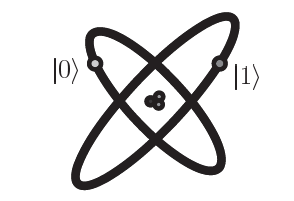
\includegraphics[width=0.5\textwidth]{Immagine1.png} 
    \caption{Qubit rappresentato da 2 livelli elettronici in un atomo.}
    \label{Immagine1}
\end{figure}
\noindent Un aspetto frequentemente discusso nell'ambito della meccanica quantistica riguarda il \textit{significato} o l'\textit{interpretazione} attribuibile agli stati di sovrapposizione e alla natura intrinsecamente probabilistica delle osservazioni relative ai sistemi quantistici. Tuttavia, nel presente elaborato tali questioni interpretative non verranno approfondite. L'obiettivo sarà piuttosto quello di sviluppare modelli concettuali e matematici utili a fini predittivi, senza entrare nel merito delle implicazioni filosofiche.
Un modello particolarmente efficace per la rappresentazione di un singolo \textbf{qubit} è quello geometrico, basato sulla cosiddetta \textbf{sfera di Bloch}.
Considerando che i coefficienti complessi $\alpha$ e $\beta$ di uno stato quantistico $\ket{\psi} = \alpha\ket{0} + \beta\ket{1}$ soddisfano la condizione di normalizzazione $|\alpha|^2 + |\beta|^2 = 1$, è possibile riscrivere lo stato in forma parametrica come segue:
\[
\ket{\psi} = e^{i\gamma} \left( \cos\frac{\theta}{2}\ket{0} + e^{i\varphi} \sin\frac{\theta}{2}\ket{1} \right),
\]
dove $\theta$, $\varphi$ e $\gamma$ sono parametri reali.
Il fattore globale di fase $e^{i\gamma}$ non ha conseguenze osservabili sulle misurazioni e, pertanto, può essere trascurato senza perdita di generalità. Lo stato può dunque essere efficacemente espresso nella forma:
\[
\ket{\psi} = \cos\frac{\theta}{2}\ket{0} + e^{i\varphi} \sin\frac{\theta}{2}\ket{1}.
\]
Questa parametrizzazione consente di interpretare lo stato di un qubit come un punto sulla superficie della sfera unitaria tridimensionale, nota come \textbf{sfera di Bloch}. Tale rappresentazione fornisce uno strumento intuitivo e potente per visualizzare gli stati di singoli qubit ed è particolarmente utile per l'analisi qualitativa delle operazioni quantistiche elementari. Tuttavia, si sottolinea che l'utilità della sfera di Bloch è limitata ai sistemi a un solo qubit, in quanto non esiste una generalizzazione semplice e diretta di tale rappresentazione per sistemi composti da più qubit.
\begin{figure}[H]
    \centering
    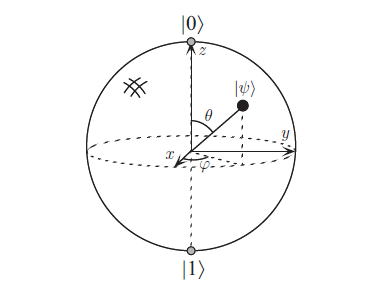
\includegraphics[width=0.5\textwidth]{Immagine2.png} 
    \caption{Rappresentazione di un qubit sulla sfera di Bloch.}
    \label{Immagine2}
\end{figure}
\noindent Una questione fondamentale nell'ambito dell'informazione quantistica riguarda la quantità di informazione rappresentata da un singolo \textbf{qubit}. A prima vista, potrebbe sembrare che un qubit sia in grado di immagazzinare una quantità infinita di informazione. Infatti, poiché lo stato quantistico di un qubit può essere rappresentato da un punto arbitrario sulla superficie della sfera di Bloch, e dunque da valori continui per i parametri $\theta$ e $\varphi$, si potrebbe concludere, erroneamente, che un qubit possa contenere, in linea di principio, un numero infinito di bit. Ad esempio, l'intero contenuto di un testo letterario complesso potrebbe essere codificato nella rappresentazione binaria infinita del parametro $\theta$.
Tuttavia, tale conclusione si rivela fuorviante a causa della natura delle \textbf{misurazioni quantistiche}. Quando un qubit viene misurato, l'unico risultato possibile è uno tra due valori discreti: $0$ o $1$. Inoltre, l'atto stesso della misurazione \textbf{modifica} lo stato del qubit: esso \textbf{collassa} in uno dei due stati base $\ket{0}$ o $\ket{1}$, coerentemente con l'esito osservato. Ad esempio, se uno stato iniziale $\ket{+} = \frac{1}{\sqrt{2}}(\ket{0} + \ket{1})$ viene misurato e il risultato è $0$, lo stato post-misurazione sarà $\ket{0}$. La ragione profonda di questo fenomeno non è nota: il collasso dello stato è una conseguenza diretta dei \textbf{postulati fondamentali della meccanica quantistica}.
Ciò che risulta rilevante ai fini dell'informazione è che una \textbf{singola misurazione} di un qubit fornisce al massimo \textbf{un solo bit} di informazione. Questo fatto risolve l'apparente paradosso della "memorizzazione infinita": sebbene lo stato del qubit sia descritto da variabili continue, l'informazione effettivamente estraibile da una singola istanza è intrinsecamente limitata. Solo effettuando misurazioni su un \textbf{numero arbitrariamente grande di qubit} preparati nello stesso identico stato sarebbe possibile determinare con precisione i coefficienti complessi $\alpha$ e $\beta$ dello stato $\ket{\psi} = \alpha\ket{0} + \beta\ket{1}$.
Una domanda ancora più sottile riguarda invece l'informazione contenuta \textit{prima} della misurazione: \textit{quanta informazione rappresenta un qubit se non lo osserviamo?} A prima vista, questa può apparire come una domanda priva di senso, poiché l'informazione, per essere quantificata, deve poter essere estratta. Tuttavia, il quesito solleva un punto concettualmente cruciale: quando un sistema quantistico evolve in maniera \textbf{unitaria} -- ovvero in assenza di misurazioni o interazioni con l'ambiente -- la sua dinamica tiene conto di tutte le \textbf{variabili continue} che descrivono lo stato quantistico. In questo senso, si può affermare che \textbf{la Natura conserva e manipola una grande quantità di "informazione nascosta"} nello stato del sistema quantistico, anche se questa informazione non è direttamente accessibile tramite osservazione singola.
Tale fenomeno diventa ancora più significativo nel contesto di sistemi composti da \textbf{più qubit}: come verrà discusso nei capitoli successivi, la quantità potenziale di informazione "nascosta" o latente \textbf{cresce esponenzialmente} con il numero di qubit. Lo studio e la comprensione di questa informazione quantistica non osservabile costituiscono uno dei temi centrali dell'informazione quantistica e rappresentano il fondamento teorico del potenziale computazionale dei sistemi quantistici.
\subsubsection{Sistemi multi-qubit e la computazione quantistica}
Consideriamo un sistema costituito da \textbf{due qubit}. Nel caso classico, due bit possono assumere una delle quattro possibili configurazioni: \texttt{00}, \texttt{01}, \texttt{10} e \texttt{11}. Analogamente, nel caso quantistico, un sistema di due qubit possiede \textbf{quattro stati base computazionali}, denotati come:
\[
\ket{00}, \quad \ket{01}, \quad \ket{10}, \quad \ket{11}.
\]
Tuttavia, a differenza del caso classico, i qubit possono trovarsi in \textbf{sovrapposizioni lineari} di questi stati base. In particolare, uno stato generico di due qubit può essere descritto come:
\begin{equation}
\ket{\psi} = \alpha_{00}\ket{00} + \alpha_{01}\ket{01} + \alpha_{10}\ket{10} + \alpha_{11}\ket{11},
\end{equation}
dove i coefficienti $\alpha_{ij} \in \mathbb{C}$ rappresentano le \textbf{ampiezze} associate a ciascuno stato base, e soddisfano la \textbf{condizione di normalizzazione}:
\[
\sum_{x \in \{0,1\}^2} |\alpha_x|^2 = 1.
\]
Il risultato di una misurazione su tale stato corrisponde a uno dei quattro possibili bitstring $x \in \{00, 01, 10, 11\}$, con probabilità $|\alpha_x|^2$. Dopo la misurazione, il sistema collassa nello stato classico corrispondente $\ket{x}$.
È possibile anche effettuare una \textbf{misurazione parziale}, ad esempio osservando solo il primo qubit. In tal caso, il valore 0 viene rilevato con probabilità $|\alpha_{00}|^2 + |\alpha_{01}|^2$, e lo stato post-misura del sistema diventa:
\begin{equation}
\ket{\psi'} = \frac{\alpha_{00}\ket{00} + \alpha_{01}\ket{01}}{\sqrt{|\alpha_{00}|^2 + |\alpha_{01}|^2}},
\end{equation}
che è opportunamente rinormalizzato affinché la nuova funzione d'onda continui a rispettare la condizione di normalizzazione.
Un esempio paradigmatico di stato a due qubit è lo \textbf{stato di Bell}, anche noto come \textbf{coppia EPR} (Einstein-Podolsky-Rosen), definito da:
\begin{equation}
\ket{\Phi^+} = \frac{\ket{00} + \ket{11}}{\sqrt{2}}.
\end{equation}
Questo stato è fondamentale in molteplici protocolli dell'informazione quantistica, tra cui il \textbf{teletrasporto quantistico} e la \textbf{codifica superdensa} (discussi nelle Sezioni 1.3.7 e 2.3, rispettivamente). Esso possiede una proprietà chiave: una misurazione del primo qubit restituisce \texttt{0} con probabilità $\frac{1}{2}$, lasciando lo stato post-misura in $\ket{00}$, oppure \texttt{1} con probabilità $\frac{1}{2}$, lasciando il sistema in $\ket{11}$. In entrambi i casi, il risultato della misura sul secondo qubit sarà deterministico e uguale a quello del primo, mostrando \textbf{correlazioni perfette} tra i due qubit.
Queste correlazioni non si limitano alla base computazionale: anche altre basi di misurazione, ottenute tramite opportune trasformazioni unitarie locali (ossia applicate solo a uno dei due qubit), mostrano correlazioni non spiegabili classicamente. Tale fenomeno fu inizialmente descritto da Einstein, Podolsky e Rosen nel loro celebre articolo, e ulteriormente formalizzato da \textbf{John Bell}. Il \textbf{teorema di Bell} dimostra che le correlazioni osservabili in stati come $\ket{\Phi^+}$ sono \textbf{più forti di qualsiasi correlazione ottenibile in un sistema classico} obbediente al realismo locale. Questo risultato fornisce una prima e fondamentale indicazione della \textbf{potenza computazionale} della meccanica quantistica.
\subsubsection*{Sistemi a più qubit}
Generalizzando, un sistema composto da $n$ qubit presenta $2^n$ \textbf{stati base computazionali}, ciascuno rappresentato dalla forma $\ket{x_1 x_2 \ldots x_n}$, con $x_i \in \{0,1\}$. Di conseguenza, uno stato quantistico arbitrario del sistema è definito da $2^n$ \textbf{ampiezze complesse}, soggette a normalizzazione.
La crescita esponenziale del numero di coefficienti richiesti per descrivere lo stato quantistico rende impraticabile la sua simulazione su computer classici già per valori moderati di $n$. Per esempio, per $n = 500$, lo stato quantistico richiederebbe la gestione di $2^{500}$ numeri complessi, un numero \textbf{superiore a quello degli atomi dell'intero universo osservabile}. Tuttavia, \textbf{la Natura sembra evolvere tali stati senza difficoltà}, suggerendo che essa 'gestisca' implicitamente queste enormi strutture, come se conservasse silenziosamente una quantità astronomica di informazione 'nascosta'.
Questa caratteristica pone le basi teoriche per sfruttare i sistemi quantistici nella computazione, permettendo l'elaborazione di informazioni a una scala e con una potenza \textbf{non raggiungibili} mediante dispositivi classici.
\subsubsection{Fondamenti della computazione quantistica}
La \textbf{computazione quantistica} fornisce un quadro formale per descrivere l'evoluzione di sistemi quantistici mediante \textbf{circuiti quantistici}, analogamente a come la computazione classica è rappresentata tramite circuiti logici. Un circuito quantistico è costituito da \textbf{fili}, che trasportano qubit, e da \textbf{gate quantistici}, che eseguono trasformazioni unitarie sugli stessi.
Nei capitoli successivi saranno introdotti alcuni gate fondamentali (quali Hadamard, CNOT, Pauli-X, Z, ecc.) e verranno analizzati esempi di circuiti quantistici che evidenziano il loro impiego. Tra questi, particolare rilievo sarà dato al \textbf{circuito di teletrasporto quantistico}, che rappresenta uno degli esempi più significativi dell'utilità operativa dell'entanglement e delle correlazioni non classiche tra qubit.

\section{Gate a qubit singolo}
Nei circuiti dei computer classici, l'elaborazione delle informazioni è realizzata attraverso una combinazione di \textbf{fili}, che trasportano i segnali, e \textbf{porte logiche}, che manipolano tali segnali. Le porte logiche classiche operano su bit e, nel caso delle porte a singolo bit, l'unico elemento non banale è la \textbf{porta NOT}, la cui funzione è quella di invertire il valore del bit: secondo la sua tabella di verità, $0 \mapsto 1$ e $1 \mapsto 0$.
Nel contesto quantistico, è naturale chiedersi se esista un'analoga \textbf{porta NOT quantistica}. In tale caso, si vorrebbe definire un'operazione che trasformi lo stato base $\ket{0}$ nello stato $\ket{1}$ e viceversa. Tuttavia, poiché un \textbf{qubit} può trovarsi in \textbf{sovrapposizione} degli stati base, una semplice definizione basata sui soli vettori $\ket{0}$ e $\ket{1}$ non è sufficiente per determinare il comportamento della porta su uno stato arbitrario. È quindi necessario assumere \textbf{linearità}, una proprietà fondamentale delle trasformazioni ammesse dalla meccanica quantistica.
Assumendo la linearità, una porta NOT quantistica deve agire sullo stato generico di un qubit
\[
\ket{\psi} = \alpha\ket{0} + \beta\ket{1}
\]
trasformandolo nello stato
\[
X\ket{\psi} = \alpha\ket{1} + \beta\ket{0}.
\]
Questa trasformazione è descritta formalmente da una matrice $2 \times 2$ definita come
\[
X \equiv \begin{bmatrix}
0 & 1 \\
1 & 0
\end{bmatrix}.
\]
La notazione $X$ è storica, e rappresenta una delle tre matrici di \textbf{Pauli}, ampiamente utilizzate nella teoria dell'informazione quantistica.
Se si rappresenta lo stato $\ket{\psi}$ in notazione vettoriale come
\[
\ket{\psi} = \begin{bmatrix}
\alpha \\
\beta
\end{bmatrix},
\]
l'applicazione della porta $X$ produce il vettore
\[
X\ket{\psi} = \begin{bmatrix}
0 & 1 \\
1 & 0
\end{bmatrix}
\begin{bmatrix}
\alpha \\
\beta
\end{bmatrix}
= \begin{bmatrix}
\beta \\
\alpha
\end{bmatrix}.
\]
È importante osservare che la trasformazione associata a una porta quantistica deve preservare la \textbf{normalizzazione} dello stato quantistico. Dato uno stato $\ket{\psi} = \alpha\ket{0} + \beta\ket{1}$ tale che $|\alpha|^2 + |\beta|^2 = 1$, anche lo stato trasformato $\ket{\psi'} = U\ket{\psi}$ deve soddisfare la medesima condizione di normalizzazione. Ciò impone una restrizione fondamentale sulla matrice $U$: essa deve essere \textbf{unitaria}, ossia
\[
U^\dagger U = I,
\]
dove $U^\dagger$ indica l'aggiunto (coniugato trasposto) di $U$ e $I$ è la matrice identità $2 \times 2$. Ad esempio, nel caso della porta NOT quantistica, si verifica facilmente che:
\[
X^\dagger = X \quad \text{e} \quad X^\dagger X = XX = I.
\]
Sorprendentemente, l'\textbf{unitarietà} rappresenta l'unico vincolo per la validità di una porta quantistica su un singolo qubit. Qualsiasi matrice unitaria $2 \times 2$ definisce un'operazione fisicamente realizzabile su un qubit. Questa libertà rappresenta un marcato contrasto con il caso classico, dove le trasformazioni possibili a singolo bit sono estremamente limitate e, a parte la porta identità, la sola porta non banale è la NOT. Nel contesto quantistico, invece, lo spazio delle trasformazioni è molto più ampio e ricco, dando origine a una grande varietà di operazioni fondamentali per l'elaborazione quantistica dell'informazione.
\begin{figure}[H]
    \centering
    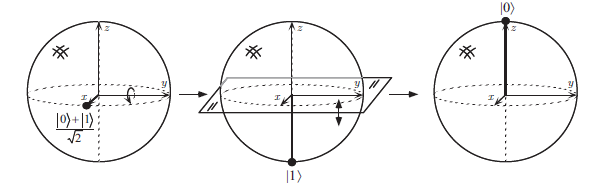
\includegraphics[width=0.6\textwidth]{Immagine3.png} 
    \caption{Visualizzazione del gate di Hadamard sulla sfera di Bloch, che agisce sullo stato di input \(\frac{\ket{0} + \ket{1}}{\sqrt{2}}\).}
    \label{Immagine3}
\end{figure}
\noindent Nel contesto dei circuiti classici, l'unica porta logica a singolo bit non banale è la porta \textbf{NOT}. Al contrario, nel paradigma quantistico esiste un'infinità di trasformazioni ammissibili a singolo qubit. Ciò è dovuto al fatto che qualsiasi matrice unitaria $2 \times 2$ può rappresentare un'operazione quantistica valida su un qubit, purché preservi la condizione di normalizzazione dello stato quantistico. Questo amplia significativamente l'insieme delle operazioni possibili rispetto al caso classico.
Un esempio di porta quantistica a singolo qubit, distinta dalla porta $X$ (NOT quantistica), è la porta $Z$, che applica una fase allo stato $\ket{1}$ lasciando invariato lo stato $\ket{0}$. Un altro esempio di particolare interesse è la \textbf{porta radice di NOT}, indicata con $\sqrt{\text{NOT}}$, definita dalla seguente matrice:
\begin{equation}
\sqrt{\text{NOT}} \equiv \frac{1}{2} \begin{bmatrix} 1+i & 1-i \\ 1-i & 1+i \end{bmatrix}.
\end{equation}
Questa porta prende il nome dal fatto che, applicandola due volte consecutivamente a un qubit, si ottiene l'equivalente dell'operazione $X$; in altre parole, $(\sqrt{\text{NOT}})^2 = X$. La verifica formale di tale identità è oggetto dell'esercizio 1.3.
Un ulteriore concetto rilevante, che evidenzia il legame tra operazioni quantistiche e misurazioni, è presentato nell'esercizio 1.4. In esso si richiede di dimostrare che una misurazione di un qubit nella base computazionale $\{ \ket{0}, \ket{1} \}$ può essere interpretata come l'applicazione di una porta \textbf{Hadamard}, seguita da una misurazione nella \textbf{base Hadamard}, ovvero $\{ \ket{+}, \ket{-} \}$, dove:
\[
\ket{+} = \frac{1}{\sqrt{2}}(\ket{0} + \ket{1}), \quad
\ket{-} = \frac{1}{\sqrt{2}}(\ket{0} - \ket{1}).
\]
Questo risultato offre una prima intuizione su come le porte quantistiche e i processi di misura siano strettamente interconnessi, ponendo le basi per lo sviluppo di circuiti quantistici più complessi, come la porta \textbf{CNOT}.
\begin{figure}[H]
    \centering
    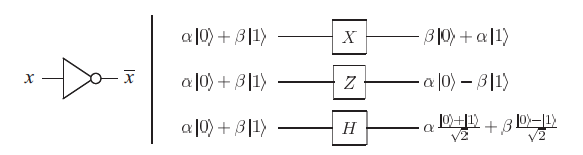
\includegraphics[width=0.7\textwidth]{Immagine4.png} 
    \caption{Singolo bit (sinistra) e porte logiche quantistiche (destra)}
    \label{Immagine4}
\end{figure}
\noindent Esistono infiniti operatori unitari $2\times 2$ e, di conseguenza, un'infinità di possibili porte quantistiche a singolo qubit. Tuttavia, le proprietà dell'intero insieme possono essere comprese a partire da un sottoinsieme molto più ristretto. In particolare, come spiegato nel \textbf{Box 1.1}, un qualunque gate unitario su singolo qubit può essere scomposto in:

\begin{enumerate}
    \item Una rotazione generica nel piano $x$--$y$, rappresentata dalla matrice
    \begin{equation}
    R(\gamma) = \begin{pmatrix}
        \cos(\tfrac{\gamma}{2}) & -\sin(\tfrac{\gamma}{2}) \\
        \sin(\tfrac{\gamma}{2}) & \cos(\tfrac{\gamma}{2})
    \end{pmatrix},
    \end{equation}
    
    \item Una rotazione attorno all'asse $\hat{z}$, data da
    \begin{equation}
    R_z(\beta) = \begin{pmatrix}
        e^{-i\beta/2} & 0 \\
        0 & e^{+i\beta/2}
    \end{pmatrix},
    \end{equation}
    
    \item Un fattore di fase globale $e^{i\alpha}$, che moltiplica l'intera matrice.
\end{enumerate}
Queste tre classi di operazioni -- rotazioni generiche, rotazioni attorno a $\hat{z}$ e shift di fase globale -- costituiscono un sistema di gate da cui, imponendo opportuni valori discreti di $\alpha$, $\beta$ e $\gamma$, è possibile \textbf{approssimare arbitrariamente bene} un qualsiasi altro gate unitario su un singolo qubit. In tal modo si ottiene un \textbf{insieme finito} di porte sufficienti a generare qualunque operazione singolo-qubit con precisione arbitraria.
Più in generale, una qualunque computazione quantistica su un qualsiasi numero di qubit può essere realizzata combinando un numero finito di porte estratte da un insieme \textbf{universale} per la computazione quantistica. Prima di introdurre la universalità a più qubit, è tuttavia utile richiamare formalmente la decomposizione a singolo qubit:

\begin{center}
\fbox{
\begin{minipage}{0.95\textwidth}
    \textbf{Box 1.1 -- Decomposizione delle operazioni a singolo qubit} \\
    In precedenza abbiamo dimostrato che un qualunque operatore unitario $U\in U(2)$ può essere rappresentato come
    \begin{equation}
    U = e^{i\alpha}
    \begin{pmatrix}
        e^{-i\beta/2} & 0 \\
        0 & e^{+i\beta/2}
    \end{pmatrix}
    \begin{pmatrix}
        \cos(\tfrac{\gamma}{2}) & -\sin(\tfrac{\gamma}{2}) \\
        \sin(\tfrac{\gamma}{2}) & \cos(\tfrac{\gamma}{2})
    \end{pmatrix}
    \begin{pmatrix}
        e^{-i\delta/2} & 0 \\
        0 & e^{+i\delta/2}
    \end{pmatrix}.
    \end{equation}
    dove $\alpha,\beta,\gamma,\delta\in\mathbb{R}$.
    
    Si noti che la matrice centrale è una rotazione nel piano, mentre le prime e ultime matrici possono anch'esse essere interpretate come rotazioni in piani differenti. Questa decomposizione fornisce una \textbf{ricetta esatta} per realizzare arbitrariamente qualsiasi porta quantistica su singolo qubit.
\end{minipage}
}
\end{center}
In tal modo, l'insieme costituito da questi tre tipi di gate -- insieme a un opportuno set discreto di parametri $\{\alpha,\beta,\gamma,\delta\}$ -- è \textbf{universale} per le operazioni a singolo qubit. Nelle sezioni successive verranno poi introdotti i gate multi-qubit necessari a estendere tale universalità all'intera computazione quantistica.

\section{Gate a più qubit}
Estendendo il discorso da un singolo qubit a sistemi multi-qubit, in Figura 1.6 sono illustrate cinque porte logiche classiche a più bit di uso comune: AND, OR, NAND, XOR ed NOR. Un risultato fondamentale della teoria della computazione classica è che \textbf{qualsiasi} funzione booleana può essere realizzata mediante la composizione di sole porte NAND (o, in alternativa, sole porte NOR): tali porte sono pertanto dette \textbf{universali}. Al contrario, la porta AND da sola -- o anche in combinazione con la porta OR -- non è universale, poiché entrambe preservano la \textbf{parità} complessiva dei bit: un circuito composto unicamente da porte AND e OR restituirà sempre in uscita stringhe di pari parità rispetto a quelle delle coppie di ingressi a parità uguale, limitando la classe delle funzioni computabili.
L'analogo quantistico della porta multi-bit è la \textbf{porta controllata-NOT} (o CNOT). Essa agisce su due qubit, detti rispettivamente \textbf{controllo} e \textbf{bersaglio}, e si rappresenta in circuito come:
\begin{center}
    \texttt{---$\bullet$---} \quad controllo \\
    \texttt{---$\oplus$---} \quad bersaglio
\end{center}
\begin{figure}[H]
    \centering
    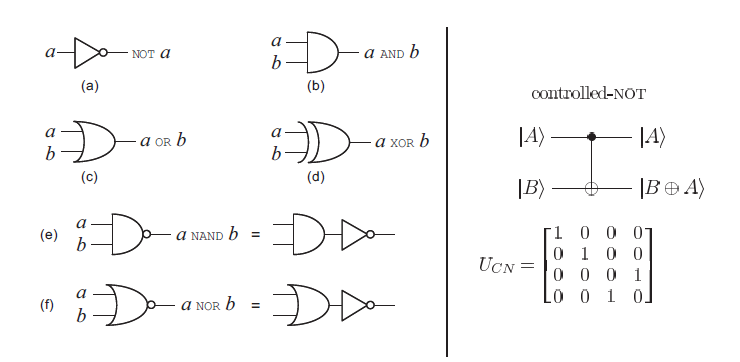
\includegraphics[width=0.9\textwidth]{Immagine5.png} 
    \caption{Corrispondeze tra porte classiche e quantistiche.}
    \label{Immagine5}
\end{figure}
L'azione sulla base computazionale è definita da:
\begin{equation}
\begin{aligned}
    &|00\rangle \mapsto |00\rangle, \quad |01\rangle \mapsto |01\rangle, \\
    &|10\rangle \mapsto |11\rangle, \quad |11\rangle \mapsto |10\rangle.
\end{aligned}
\end{equation}
In altre parole, se il qubit di controllo vale $0$, il qubit bersaglio rimane invariato; se vale $1$, il qubit bersaglio viene invertito (operazione XOR modulo 2).
Matematicamente, la porta CNOT può essere vista come un'estensione unitaria della porta classica XOR:
\[
|A,B\rangle \;\mapsto\; |A,\,B \oplus A\rangle,
\]
dove $\oplus$ indica l'addizione modulo 2. La matrice $4\times4$ corrispondente, che agisce sul vettore $(\alpha_{00},\alpha_{01},\alpha_{10},\alpha_{11})^\mathsf{T}$, è unitaria, ovvero
\[
U_{\mathrm{CNOT}}^\dagger\,U_{\mathrm{CNOT}} \;=\; I_4.
\]
Poiché le porte classiche come AND e OR sono \textbf{irreversibili} (e quindi non invertibili), non esiste alcuna loro rappresentazione unitaria: la perdita di informazione intrinseca in una NAND classica (ad esempio, non potendo risalire univocamente agli ingressi a partire dall'uscita) rende impossibile la loro realizzazione mediante operatori unitarî. Al contrario, ogni porta quantistica -- essendo descritta da una matrice unitaria -- è \textbf{per definizione} invertibile, e la sua inversa è anch'essa una porta quantistica.
Un fondamentale risultato sulla \textbf{universalità} in ambito quantistico afferma che:
\vspace{0.3cm}
\noindent\fbox{\parbox{0.95\textwidth}{%
    \textbf{Ogni} gate logico su più qubit può essere implementato tramite composizione di porte CNOT e di opportune porte a singolo qubit.
}}
\vspace{0.3cm}
\noindent La dimostrazione è l'analogo quantistico della proprietà di universalità della porta NAND in logica classica.
\subsection*{1.3.3 Misurazioni in basi diverse da quella computazionale}
Finora abbiamo descritto le misurazioni di un singolo qubit espresse nella \textbf{base computazionale} $\{|0\rangle,|1\rangle\}$: uno stato generico
\[
|\psi\rangle = \alpha|0\rangle + \beta|1\rangle
\]
viene misurato restituendo il risultato ``0'' con probabilità $|\alpha|^2$, oppure ``1'' con probabilità $|\beta|^2$, e collassando il qubit nello stato corrispondente.
Tuttavia, la meccanica quantistica consente di misurare in \textbf{qualsiasi} base ortonormale. Ad esempio, nella \textbf{base di Hadamard}
\[
|+\rangle \equiv \tfrac{1}{\sqrt{2}}(|0\rangle+|1\rangle), \qquad
|-\rangle \equiv \tfrac{1}{\sqrt{2}}(|0\rangle-|1\rangle),
\]
uno stato arbitrario si riscrive come:
\begin{equation}
|\psi\rangle
= \alpha|0\rangle+\beta|1\rangle
= \frac{\alpha+\beta}{\sqrt{2}}\,|+\rangle
+ \frac{\alpha-\beta}{\sqrt{2}}\,|-\rangle.
\end{equation}
Una misurazione in questa base darà ``$+$'' con probabilità $\left|\tfrac{\alpha+\beta}{\sqrt{2}}\right|^2$ e ``$-$'' con probabilità $\left|\tfrac{\alpha-\beta}{\sqrt{2}}\right|^2$, collassando il qubit rispettivamente in $|+\rangle$ o $|-\rangle$.
In generale, data qualunque base ortonormale $\{|a\rangle,|b\rangle\}$, uno stato
$\alpha|a\rangle+\beta|b\rangle$ può essere misurato in tale base con probabilità $|\alpha|^2$ e $|\beta|^2$, a condizione che $\langle a|b\rangle=0$. Il vincolo di ortonormalità garantisce che le probabilità sommino a uno.
Analoghe generalizzazioni valgono per misurazioni di sistemi multi-qubit in basi arbitrariamente scelte. Dal punto di vista teorico, qualsiasi base ortonormale su $2^n$ dimensioni può essere misurata, ma la \textbf{complessità} e l'\textbf{efficienza} con cui tale misurazione può essere realizzata fisicamente dipendono dalla struttura specifica della base scelta.

\section{Circuiti elementari}
Abbiamo già introdotto alcuni circuiti quantistici elementari. Per comprendere meglio la loro struttura, consideriamo in dettaglio il circuito mostrato in Figura 1.7, composto da tre porte quantistiche. Il circuito si legge da sinistra verso destra e ciascuna linea orizzontale rappresenta un ``filo'' del circuito quantistico. Tale filo non deve necessariamente corrispondere a un conduttore elettrico: può indicare, ad esempio, il flusso temporale di un singolo qubit o il percorso spaziale di una particella---come un fotone---che si propaga da un dispositivo all'altro.
Per convenzione, l'ingresso di un circuito quantistico è spesso assunto essere uno \textbf{stato base computazionale}, tipicamente $\ket{0\,0\,\dots\,0}$. In letteratura possono trovarsi varie eccezioni a questa regola, ma è buona norma segnalarle esplicitamente al lettore quando lo stato iniziale differisce da quello convenzionale.
Il circuito di Figura 1.7 realizza l'operazione di \textbf{swap}, ovvero scambia gli stati di due qubit distinti. Per verificarlo, si osservi l'effetto sequenziale delle tre porte controllate-NOT sul generico stato base computazionale $\ket{a,b}$, con $a,b\in\{0,1\}$. Indicando con $\oplus$ l'addizione modulo 2, si ha:
\begin{equation}
\begin{aligned}
\ket{a,b} 
&\;\xrightarrow{\;\mathrm{CNOT}_{1\to2}\;} 
\ket{a,\;a \oplus b},\\
&\;\xrightarrow{\;\mathrm{CNOT}_{2\to1}\;} 
\ket{a \oplus (a \oplus b),\;a \oplus b}
   = \ket{b,\;a \oplus b},\\
&\;\xrightarrow{\;\mathrm{CNOT}_{1\to2}\;} 
\ket{b,\;(a \oplus b)\oplus b}
   = \ket{b,\;a}.
\end{aligned}
\end{equation}
In ciascuno di questi tre passi, le porte CNOT sono direzionate rispettivamente dal primo qubit verso il secondo ($\mathrm{CNOT}_{1\to2}$), dal secondo verso il primo ($\mathrm{CNOT}_{2\to1}$) e nuovamente dal primo verso il secondo. Al termine della sequenza, il qubit 1 contiene $b$ e il qubit 2 contiene $a$, cioè gli stati originali sono stati \textbf{scambiati}, come previsto dall'operazione di \textit{swap}.
Questa costruzione dimostra come un compito apparentemente complesso---lo scambio di due registri quantistici---possa essere realizzato con una \textbf{sequenza di gate universali} (in questo caso, tre CNOT), confermando in pratica l'importanza della porta CNOT quale elemento base nella progettazione dei circuiti quantistici.
\begin{figure}[H]
    \centering
    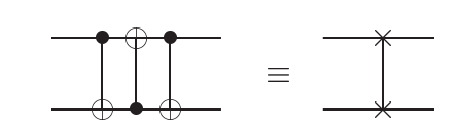
\includegraphics[width=0.6\textwidth]{Immagine6.png} 
    \caption{Circuito che scambia due qubit e una notazione schematica equivalente per questo circuito comune e utile.}
    \label{Immagine6}
\end{figure}
\noindent Nella realizzazione di circuiti quantistici, vanno tenute presenti alcune importanti differenze rispetto ai circuiti classici:
\begin{enumerate}[leftmargin=*, labelwidth=\widthof{\bfseries Divieto di duplicazione}, label=\textbf{\arabic*.}]
    \item \textbf{Assenza di ciclicità} \\
    Nei circuiti quantistici non sono ammessi \textbf{feedback} né \textbf{loop}: il grafo delle porte deve essere \textbf{acyclic}, ossia privo di cicli, in modo che il flusso dell'informazione quantistica proceda in un'unica direzione temporale.
    
    \item \textbf{Divieto di unioni di fili} \\
    Nei circuiti classici è permessa l'operazione di \textbf{OR} o di \textbf{wired-OR}, per cui più segnali di ingresso vengono "uniti" in un unico filo tramite un'operazione di bitwise-OR. Tale trasformazione non è \textbf{reversibile} e quindi non corrisponde a un'operazione unitaria: di conseguenza, \textbf{non è consentita} nei circuiti quantistici.
    
    \item \textbf{Divieto di duplicazione} \\
    L'operazione inversa dell'unione, cioè la \textbf{duplicazione} di un bit in più copie, è anch'essa irreversibile. In misura ancora più stringente, la meccanica quantistica vieta la duplicazione arbitraria di un qubit (no-cloning theorem): \textbf{non esiste} alcun circuito quantistico in grado di copiare un qubit sconosciuto in modo perfetto. 
    \begin{equation}
        \ket{\psi}\ket{0} \;\longmapsto\; \ket{\psi}\ket{\psi},
    \end{equation}
    per uno stato generico $\ket{\psi}$.
\end{enumerate}
\vspace{1em}
\noindent\rule{\textwidth}{0.4pt}
\vspace{1em}
Per introdurre porte quantistiche più complesse, conviene adottare la seguente \textbf{convenzione grafica} (Figura 1.8): sia $U$ un qualunque operatore unitario che agisca su $n$ qubit. Possiamo definire il \textbf{controlled-$U$}, ovvero un gate con:
\begin{figure}[H]
    \centering
    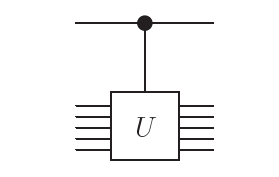
\includegraphics[width=0.6\textwidth]{Immagine7.png} 
    \caption{Controlled-U gate.}
    \label{Immagine7}
\end{figure}
\begin{itemize}
    \item un \textbf{qubit di controllo}, rappresentato da una linea con un \textbf{pallino nero};
    \item $n$ \textbf{qubit di destinazione}, indicati da un riquadro con scritto $U$.
\end{itemize}
L'azione del controlled-$U$ è la seguente:
\begin{itemize}
    \item se il qubit di controllo è $\ket{0}$, i $n$ qubit di destinazione restano invariati;
    \item se il qubit di controllo è $\ket{1}$, l'operatore $U$ viene applicato alle linee di destinazione.
\end{itemize}
Il caso più importante è il \textbf{controlled-NOT}, ottenuto ponendo $U = X$ (Figura 1.9), che coincide con la porta CNOT già introdotta.
\begin{figure}[H]
    \centering
    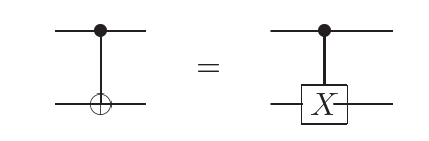
\includegraphics[width=0.6\textwidth]{Immagine8.png} 
    \caption{Due diverse rappresentazioni della porta NOT-controllata}
    \label{Immagine8}
\end{figure}
Infine, per rappresentare un'operazione di \textbf{misura}, si utilizza il simbolo del \textbf{misuratore} (Figura 1.10). Tale operazione trasforma uno stato quantistico
\begin{equation}
    \ket{\psi} = \alpha\ket{0} + \beta\ket{1}
\end{equation}
in un \textbf{bit classico} $M$ — disegnato con un doppio filo per indicare la natura non-quantistica — che assume valore
\begin{equation}
    M = \begin{cases}
        0 & \text{con probabilità } |\alpha|^2, \\
        1 & \text{con probabilità } |\beta|^2.
    \end{cases}
\end{equation}
Lo stato post-misura collassa nel corrispondente $\ket{0}$ o $\ket{1}$.
Queste regole vincolano la progettazione dei circuiti quantistici e riflettono le proprietà unitarie e reversibili della dinamica quantistica, nonché la natura intrinsecamente distruttiva della misura.
\begin{figure}[H]
    \centering
    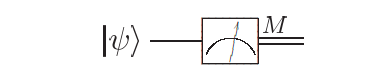
\includegraphics[width=0.6\textwidth]{Immagine10.png} 
    \caption{Simboli per le misurazioni di un circuito quantistico.}
    \label{Immagine10}
\end{figure}
\noindent Troveremo i circuiti quantistici utili come modelli per tutti i processi quantistici, non solo per il calcolo e la comunicazione, ma anche per la descrizione del rumore quantistico. Nei paragrafi seguenti vengono presentati alcuni esempi elementari a tal fine.

\subsubsection{Impossibilità di copiare un qubit (no-cloning theorem)}
Un esempio particolarmente istruttivo per illustrare una proprietà fondamentale dell'informazione quantistica è il \textbf{copiare} un bit. In ambito classico, tale operazione si realizza agevolmente mediante un gate che prende in ingresso:
\begin{enumerate}
    \item Il bit da copiare, in uno stato ignoto $x\in\{0,1\}$.
    \item Un bit ``di appoggio'' inizializzato a zero.
\end{enumerate}
\begin{figure}[H]
    \centering
    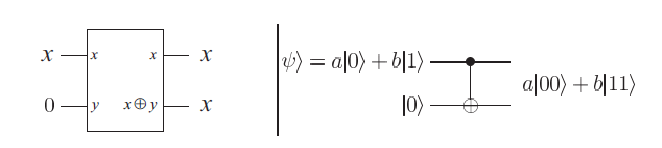
\includegraphics[width=0.6\textwidth]{Immagine11.png} 
    \caption{Circuito classico e quantistico per 'copiare' bit o qubit sconosciuto.}
    \label{Immagine11}
\end{figure}
Applicando il gate, si ottiene in uscita una coppia di bit entrambi uguali a $x$ (Figura 1.11).
Tentiamo ora di ripetere lo stesso schema per un qubit. Siano i due qubit di ingresso nello stato
\begin{equation}
\ket{\psi}\otimes\ket{0}
\;=\;
\bigl(a\ket{0} + b\ket{1}\bigr)\otimes \ket{0}
\;=\;
a\ket{00} + b\ket{10},
\end{equation}
con $\lvert a\rvert^2 + \lvert b\rvert^2 = 1$. Supponiamo di applicare allo schema un gate equivalente alla CNOT, in modo da invertire il secondo qubit solo se il primo è $\ket{1}$. L'uscita del circuito sarà quindi:
\[
a\ket{00} + b\ket{11}.
\]
Ci siamo dunque illusi di aver prodotto lo stato $\ket{\psi}\otimes\ket{\psi}$? In realtà, per uno stato puramente classico $\ket{\psi}=\ket{0}$ o $\ket{1}$, tale copia funziona correttamente. Ma per uno stato generico
\begin{equation}
\ket{\psi}\otimes\ket{\psi}
= a^2\ket{00}
+ ab\ket{01}
+ ab\ket{10}
+ b^2\ket{11},
\end{equation}
si nota immediatamente che, a meno che $ab=0$, i termini misti $\ket{01}$ e $\ket{10}$ sono non nulli. Confrontando con $a\ket{00} + b\ket{11}$, si vede che il circuito non ha effettivamente duplicato $\ket{\psi}$.
\begin{tcolorbox}[colback=white,colframe=black,arc=0mm,boxsep=5pt,left=5pt,right=5pt,top=3pt,bottom=3pt]
\textbf{Teorema del no-cloning:} Risulta \textbf{impossibile} realizzare un dispositivo quantistico che, a partire da un qubit in uno stato arbitrario sconosciuto $\ket{\psi}$ e da un qubit di appoggio $\ket{0}$, produca in uscita lo stato $\ket{\psi}\otimes\ket{\psi}$.
\end{tcolorbox}
\noindent Questo risultato è una delle differenze più marcate tra informazione classica e informazione quantistica.
Un ulteriore argomento intuitivo sul fallimento del ``circuito copia'' è basato sull'idea che un qubit contenga informazioni ``nascoste'' non direttamente accessibili tramite un'unica misurazione. Consideriamo infatti lo stato
\[
\ket{\Phi} = a\ket{00} + b\ket{11},
\]
ottenuto dal presunto ``copia-circuito'' applicato a $\ket{\psi}\otimes\ket{0}$. Misurando uno dei due qubit in base computazionale, si ottiene 0 con probabilità $\lvert a\rvert^2$ o 1 con probabilità $\lvert b\rvert^2$. Dopo la misura, il secondo qubit viene proiettato in modo deterministico su $\ket{0}$ o $\ket{1}$, e \textbf{non} rimane alcuna traccia residua delle ampiezze generiche $a$ e $b$. Analogamente, misurando il qubit originale $\ket{\psi}$ prima della duplicazione, si perderebbe ogni informazione su $a$ e $b$. Se fosse stato possibile copiare $\ket{\psi}$, la copia avrebbe dovuto conservare parte di quell'informazione ``nascosta''; poiché ciò non accade, deduciamo che nessun processo fisicamente ammissibile può duplicare uno stato quantistico arbitrario.
\vspace{1em}
\noindent\rule{\textwidth}{0.4pt}
\vspace{1em}
Questa proprietà, resa rigorosamente formale dal teorema del no-cloning, costituisce un cardine dell'informazione quantistica e sarà a più riprese utilizzata nei capitoli successivi.

\subsubsection{Esempio: stati di Bell}
Consideriamo ora un circuito leggermente più complesso, illustrato in Figura 1.12, che combina un gate di Hadamard applicato al primo qubit e successivamente una porta CNOT con primo qubit di controllo e secondo qubit bersaglio. Tale circuito trasforma i quattro stati base computazionali $\lvert ab\rangle$ ($a,b\in\{0,1\}$) nei cosiddetti \textbf{stati di Bell}, secondo la seguente tabella:

\begin{enumerate}
\item Per $\lvert 00\rangle$:
Il gate di Hadamard sul primo qubit produce
\[
H\lvert 0\rangle \otimes \lvert 0\rangle = \frac{\lvert 0\rangle + \lvert 1\rangle}{\sqrt{2}}\otimes\lvert 0\rangle = \frac{\lvert 00\rangle + \lvert 10\rangle}{\sqrt{2}}.
\]
Appena la porta CNOT agisce su questo stato, si inverte il secondo qubit solo quando il primo è $\lvert1\rangle$, ottenendo
\[
\frac{\lvert 00\rangle + \lvert 11\rangle}{\sqrt{2}} \equiv \lvert\beta_{00}\rangle.
\]
\item Per $\lvert 01\rangle$:
\[
H\lvert 0\rangle\lvert 1\rangle = \frac{\lvert 0\rangle + \lvert 1\rangle}{\sqrt{2}}\otimes \lvert 1\rangle = \frac{\lvert 01\rangle + \lvert 11\rangle}{\sqrt{2}},
\]
su cui CNOT produce
\[
\frac{\lvert 01\rangle + \lvert 10\rangle}{\sqrt{2}} \equiv \lvert\beta_{01}\rangle.
\]
\item Per $\lvert 10\rangle$:
Il gate di Hadamard trasforma il primo qubit $\lvert 1\rangle$ in $\tfrac{\lvert0\rangle - \lvert1\rangle}{\sqrt2}$, per cui
\[
H\lvert 1\rangle\lvert 0\rangle = \frac{\lvert 00\rangle - \lvert 10\rangle}{\sqrt{2}},
\]
e la CNOT dà
\[
\frac{\lvert 00\rangle - \lvert 11\rangle}{\sqrt{2}} \equiv \lvert\beta_{10}\rangle.
\]
\item Per $\lvert 11\rangle$:
\[
H\lvert 1\rangle\lvert 1\rangle = \frac{\lvert 01\rangle - \lvert 11\rangle}{\sqrt{2}},
\]
su cui CNOT produce
\[
\frac{\lvert 01\rangle - \lvert 10\rangle}{\sqrt{2}} \equiv \lvert\beta_{11}\rangle.
\]
\end{enumerate}
Gli stati $\lvert\beta_{00}\rangle,\lvert\beta_{01}\rangle,\lvert\beta_{10}\rangle,\lvert\beta_{11}\rangle$ sono noti come \textbf{stati di Bell} (o coppie EPR, da Einstein–Podolsky–Rosen–Bell) e si possono esprimere in forma compatta come:
\[
\lvert\beta_{xy}\rangle \equiv \frac{\lvert 0,y\rangle + (-1)^{x}\lvert 1,\bar y\rangle}{\sqrt{2}},
\]
dove $x,y\in\{0,1\}$ e $\bar y$ indica la negazione logica di $y$.
Questa costruzione mostra come, a partire dalla semplice composizione di un gate Hadamard e di un gate CNOT, si possano generare i quattro stati massimamente entangled (gli stati di Bell), che costituiscono un elemento fondamentale in numerosi protocolli di informazione quantistica.
\begin{figure}[H]
    \centering
    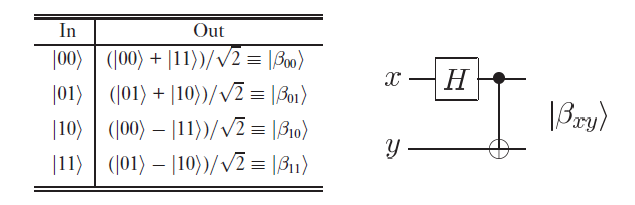
\includegraphics[width=0.9\textwidth]{Immagine12.png} 
    \caption{Circuito quantistico per creare gli stati di Bell e la tabella di verità dell'input/output.}
    \label{Immagine12}
\end{figure}


\chapter{Algoritmi quantistici fondamentali}
Una domanda centrale è la seguente: \textbf{quale classe di computazioni} può essere eseguita tramite circuiti quantistici, e come essa si confronta con la classe di computazioni realizzabili mediante circuiti logici classici? Esistono problemi in cui un computer quantistico offre un vantaggio rispetto a un computer classico? In questa sezione esamineremo tali quesiti, mostrando innanzitutto come simulare computazioni classiche su un computer quantistico, quindi illustrando alcuni esempi di problemi per i quali i computer quantistici sono più efficienti, e infine riassumendo gli algoritmi quantistici più noti.
\subsubsection{Simulazione di computazioni classiche con circuiti quantistici}
È possibile simulare un circuito logico classico mediante un circuito quantistico? Come ci si attende, la risposta è \textbf{sì}, poiché si ritiene che ogni aspetto della realtà—\newline—compresi i circuiti classici—possa essere descritto mediante meccanica quantistica. Il principale ostacolo risiede nel fatto che le porte quantistiche unitarie sono \textbf{reversibili} per definizione, mentre molte porte classiche—come la porta NAND o la porta AND—sono \textbf{irreversibili}.
Tuttavia, ogni circuito classico può essere trasformato in un circuito \textbf{reversibile} mediante l'introduzione di porte quantistiche universali. In particolare, la porta di \textbf{Toffoli} (o porta CCNOT) è una porta classica a tre bit che è essa stessa reversibile. Essa prende in input tre bit $(a,b,c)$ e restituisce in output
\[
(a,b,c \oplus (a \land b)),
\]
dove $a$ e $b$ sono i \textbf{bit di controllo} (che rimangono invariati), $c$ è il \textbf{bit bersaglio}, $\land$ indica l'AND logico e $\oplus$ l'XOR modulo 2. Poiché l'operazione di Toffoli è involutoria,
\[
\mathrm{Toffoli}^2 = \mathrm{Id},
\]
essa è \textbf{inversa di se stessa} e pertanto costituisce una porta quantistica unitaria.
È noto che la sola porta di Toffoli, eventualmente affiancata da porte a singolo qubit come Hadamard e fasi, è \textbf{universale} per la computazione classica reversibile. Quindi, sostituendo ciascuna porta irreversibile di un circuito classico con un corrispondente sottocircuito a porte di Toffoli (e porte ausiliarie), si ottiene un circuito quantistico in grado di replicare esattamente la medesima computazione logica.
In questo modo, \textbf{qualsiasi} algoritmo classico può essere implementato su un processore quantistico, garantendo compatibilità tra i modelli di calcolo classico e quantistico. Successivamente, esploreremo problemi in cui le estensioni quantistiche forniscono speedup—ad esempio nelle ricerche non strutturate (algoritmo di Grover) o nella fattorizzazione di interi (algoritmo di Shor)—e forniremo una panoramica delle più importanti tecniche di progettazione di algoritmi quantistici.
\begin{figure}[H]
    \centering
    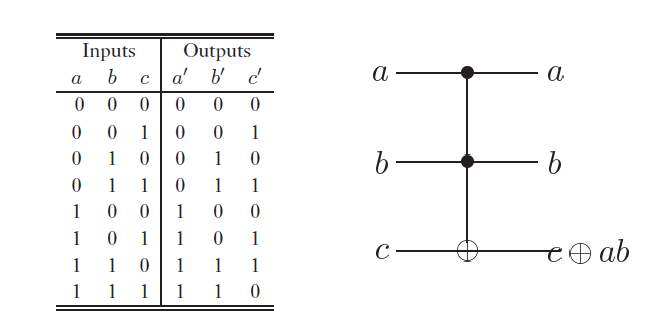
\includegraphics[width=0.9\textwidth]{Immagine13.png} 
    \caption{Tabella di verità e circuito della porta di Toffoli.}
    \label{Immagine13}
\end{figure}
\noindent Il gate di Toffoli, già introdotto come elemento fondamentale per la realizzazione di computazioni classiche reversibili, consente di simulare qualunque porta logica non reversibile. In particolare:
\begin{enumerate}
    \item \textbf{Simulazione della porta NOT} \\
    Come mostrato in Figura 1.15, è possibile realizzare un'inversione di un singolo bit utilizzando un gate di Toffoli in cui uno dei controlli è fissato a $1$ e l'altro al bit da invertire, lasciando costante il terzo bit di destinazione.

    \item \textbf{Simulazione della porta AND} \\
    Analogamente (Figura 1.16), imponendo i due qubit di controllo sui bit di input e usando un terzo qubit di destinazione inizializzato a $0$, il gate di Toffoli effettua l'operazione di AND logico, poiché il bit di destinazione viene invertito \textbf{se e solo se} entrambi i controlli sono a $1$.
\end{enumerate}
Grazie a queste due capacità, è possibile costruire un circuito reversibile di Toffoli che \textbf{simuli qualsiasi porta logica classica}—e dunque \textbf{qualsiasi} circuito classico—mediante la sola composizione di gate di Toffoli e porte ausiliarie.
Sebbene il gate di Toffoli sia stato descritto in origine nella sua versione classica, esiste una \textbf{implementazione quantistica} perfettamente equivalente. Per definizione, il \textbf{Toffoli quantistico} agisce sulla base computazionale $\{\ket{000},\dots,\ket{111}\}$ permutando gli stati esattamente come la sua controparte classica. Ad esempio,
\[
\ket{110} \mapsto \ket{111},
\]
poiché i primi due qubit di controllo sono entrambi $1$. Tale trasformazione può essere espressa mediante una matrice $8\times8$, che si verifica essere \textbf{unitaria}, confermando la legittimità del gate di Toffoli come porta quantistica.
In questo modo, i computer quantistici dotati di porte Toffoli e di porte a singolo qubit sono in grado di \textbf{eseguire qualsiasi calcolo deterministico} che un computer classico possa realizzare.
\begin{figure}[H]
    \centering
    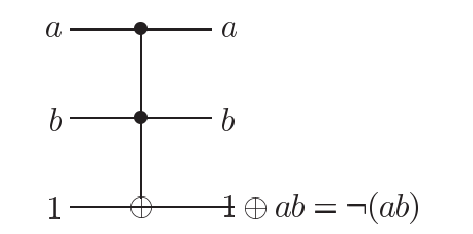
\includegraphics[width=0.6\textwidth]{Immagine14.png} 
    \caption{Classico circuito con implementazione di una porta NAND usado una porta di Toffoli.}
    \label{Immagine14}
\end{figure}
\begin{figure}[H]
    \centering
    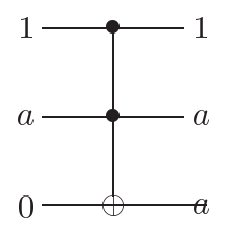
\includegraphics[width=0.3\textwidth]{Immagine15.png} 
    \caption{FANOUT con la porta di Toffoli.}
    \label{Immagine15}
\end{figure}
\subsubsection{Simulazione di calcolo non deterministico}
Un computer classico non deterministico possiede la capacità di generare bit casuali durante l'esecuzione. Anche questa caratteristica è facilmente simulabile in ambito quantistico: basta preparare un qubit nello stato $\ket{0}$, applicarvi un gate Hadamard per ottenere
\[
\frac{\ket{0} + \ket{1}}{\sqrt{2}},
\]
e infine misurare il qubit lungo la base computazionale. Il risultato sarà $0$ o $1$ con probabilità $50\%$. In tal modo il computer quantistico può \textbf{efficientemente simulare} un qualsiasi calcolo non deterministico basato su lanci di moneta equi.
\subsubsection{Oltre la simulazione classica}
Tuttavia, se la sola capacità di riprodurre computazioni classiche fosse il massimo vantaggio dei computer quantistici, non vi sarebbe ragione di ricorrere a tecnologie tanto complesse. Il vero \textbf{potenziale} della computazione quantistica risiede nella possibilità di risolvere alcuni problemi \textbf{più velocemente} di quanto non sia possibile in maniera classica. Nelle sezioni successive presenteremo algoritmi quantistici celebri, a partire dall'\textbf{algoritmo Deutsch–Jozsa}, che costituisce il primo esempio di velocizzazione quantistica provata rispetto a qualunque algoritmo classico.

\section{Parallelismo quantistico}
Il \textbf{parallelismo quantistico} costituisce l'ingrediente fondamentale di molti algoritmi quantistici. In termini heuristici---pur a rischio di semplificare eccessivamente---il parallelismo quantistico consente di valutare la stessa funzione $f(x)$ su un insieme di valori di $x$ \textbf{simultaneamente}. In questa sezione ne descriviamo il meccanismo di base e ne evidenziamo alcuni limiti.
Sia dunque
\[
f\colon\{0,1\} \to \{0,1\}
\]
una funzione booleana a bit singolo. Per rappresentarla in un circuito quantistico, consideriamo un sistema di due qubit inizialmente nello stato
\[
\ket{x,y}, \qquad x,y\in\{0,1\}.
\]
Definiamo un'operazione quantistica
\[
U_f\colon \ket{x,y} \longmapsto \ket{x,\; y \oplus f(x)},
\]
dove $\oplus$ denota l'addizione modulo 2. Il primo qubit costituisce il \textbf{registro dati} (data register), mentre il secondo è il \textbf{registro bersaglio} (target register). È immediato verificare che $U_f$ è un operatore lineare e unitario, poiché effettua una permutazione degli stati base computazionali.
Se si imposta $y=0$ all'ingresso, l'uscita del secondo qubit fornisce esattamente il valore $f(x)$. In altre parole, il circuito
\[
\ket{x,0} \xrightarrow{U_f} \ket{x,\,f(x)}
\]
realizza la \textbf{valutazione quantistica} della funzione.
Dimostreremo in segiuto che, data una descrizione classica efficiente di $f$, è possibile costruire un circuito quantistico di complessità comparabile che realizza $U_f$. Per ora, possiamo trattare $U_f$ come un \textbf{"cassetto nero"} (oracle) che calcola $f$ in modo unitario e reversibile.
Il parallelismo quantistico sorge quando si prepara il registro dati in \textbf{sovrapposizione} di tutti i possibili valori di $x$, ad esempio tramite un gate Hadamard applicato al primo qubit:
\[
\frac{\ket{0} + \ket{1}}{\sqrt{2}} \otimes \ket{0}
\xrightarrow{\,U_f\,}
\frac{\ket{0,f(0)} + \ket{1,f(1)}}{\sqrt{2}}.
\]
In un solo passo unitario, $U_f$ ha valutato simultaneamente $f(0)$ e $f(1)$. Le tecniche successive di interferenza e misura consentono tuttavia di estrarre dalle ampiezze risultanti informazioni aggregate su $f$, piuttosto che i singoli valori. In tal modo, il parallelismo quantistico può portare a \textbf{speedup} rispetto ai metodi classici per particolari problemi, come vedremo negli algoritmi di Deutsch--Jozsa, Grover e Shor.
\begin{figure}[H]
    \centering
    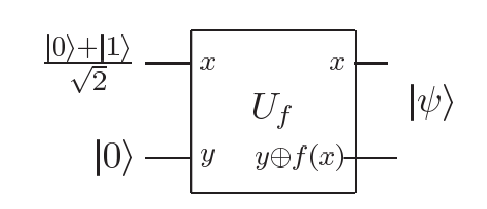
\includegraphics[width=0.5\textwidth]{Immagine16.png} 
    \caption{Circuito quantistico per la valutazione di \textit{f}(0) ed \textit{f}(1) contemporaneamente.}
    \label{Immagine16}
\end{figure}
\noindent Consideriamo il circuito descritto in Figura 1.17, nel quale l'oracolo unitario $U_f$ viene applicato non a uno stato elementare della base computazionale, bensì a una sovrapposizione. In particolare:
\begin{enumerate}
    \item \textbf{Preparazione dello stato} \\
    Il \textbf{registro dati} (primo qubit) è inizializzato in $\ket{0}$ e sottoposto a un gate di Hadamard, ottenendo
    
    \[
    H\ket{0} = \frac{\ket{0} + \ket{1}}{\sqrt{2}}.
    \]
    
    Il \textbf{registro bersaglio} (secondo qubit) resta inizializzato in $\ket{0}$.
    
    \item \textbf{Applicazione dell'oracolo $U_f$} \\
    L'operatore $U_f$ agisce sullo stato
    $\frac{1}{\sqrt{2}}\bigl(\ket{0,0} + \ket{1,0}\bigr)$,
    producendo
    
    \begin{equation}
    U_f\;\frac{\ket{0,0} + \ket{1,0}}{\sqrt{2}}
    = 
    \frac{\ket{0,f(0)} + \ket{1,f(1)}}{\sqrt{2}}.
    \end{equation}
    
    In questo modo i valori $f(0)$ e $f(1)$ appaiono \textbf{contemporaneamente} nelle diverse componenti della sovrapposizione: è il fenomeno noto come \textbf{parallelismo quantistico}.
\end{enumerate}
Tale procedura si estende agevolmente a funzioni definite su \textbf{$n$ bit}. Si introduce la \textbf{trasformata di Hadamard su $n$ qubit}, spesso detta anche \textbf{Walsh--Hadamard}, definita come
\[
H^{\otimes n} = H \otimes H \otimes \cdots \otimes H
\quad(\text{$n$ fattori}).
\]
Per $n=2$, applicando $H^{\otimes2}$ al doppio qubit $\ket{00}$ si ottiene
\begin{equation}
H^{\otimes2}\ket{00}
= 
\biggl(\frac{\ket{0} + \ket{1}}{\sqrt{2}}\biggr)
\otimes
\biggl(\frac{\ket{0} + \ket{1}}{\sqrt{2}}\biggr)
= 
\frac{\ket{00} + \ket{01} + \ket{10} + \ket{11}}{2}.
\end{equation}
In forma generale, per $n$ qubit inizializzati tutti in $\ket{0}$, si ha
\begin{equation}
H^{\otimes n}\ket{0}^{\otimes n}
= 
\frac{1}{\sqrt{2^n}}\sum_{x\in\{0,1\}^n}\ket{x},
\end{equation}
ovvero la trasformata di Hadamard produce con \textbf{complessità lineare} in $n$ una \textbf{sovrapposizione uniforme} di tutte le $2^n$ stringhe della base computazionale.
Grazie a questa trasformazione, un successivo applicazione di $U_f$ su $\ket{x}\otimes\ket{0}$ genera in un solo passo unitario la sovrapposizione
\[
\frac{1}{\sqrt{2^n}}
\sum_{x\in\{0,1\}^n}\ket{x,f(x)},
\]
costituendo la base operativa del parallelismo quantistico in tutti gli algoritmi a oracolo. Tuttavia, come vedremo, per ottenere effettivi miglioramenti di complessità è necessario sfruttare ulteriori passaggi di interferenza e misura nei passi successivi.
\begin{figure}[H]
    \centering
    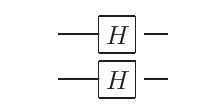
\includegraphics[width=0.5\textwidth]{Immagine17.png} 
    \caption{Trasformazione di Hadamard $H^{\otimes 2}$ su 2 qubits.}
    \label{Immagine17}
\end{figure}
\noindent L'\textbf{evaluazione parallela quantistica} di una funzione
\[
f\colon\{0,1\}^n \to \{0,1\}
\]
si realizza nei passi seguenti:
\begin{enumerate}
    \item \textbf{Inizializzazione} \\
    Si prepara il registro dati di $n$ qubit nello stato $\ket{0}^{\otimes n}$ e un qubit bersaglio in $\ket{0}$, ottenendo il vettore
    
    \[
      \ket{0}^{\otimes n} \otimes \ket{0}.
    \]
    
    \item \textbf{Trasformata di Hadamard} \\
    Si applica il gate $H^{\otimes n}$ ai primi $n$ qubit, producendo la sovrapposizione uniforme di tutte le stringhe di bit:
    
    \[
      H^{\otimes n} \ket{0}^{\otimes n}
      = \frac{1}{\sqrt{2^n}} \sum_{x \in \{0,1\}^n} \ket{x}.
    \]
    
    \item \textbf{Oracolo $U_f$} \\
    Si invoca il circuito quantistico che implementa
    
    \[
      U_f\colon \ket{x,y} \longmapsto \ket{x, y \oplus f(x)}
    \]
    
    sullo stato ottenuto, con $y=0$. Il risultato complessivo è
    
    \begin{equation}
      U_f \bigl( (H^{\otimes n} \otimes I) \, \ket{0}^{\otimes (n+1)} \bigr)
      = 
      \frac{1}{\sqrt{2^n}}
      \sum_{x \in \{0,1\}^n} \ket{x, f(x)}.
    \end{equation}
\end{enumerate}
In tal modo il circuito ha \textbf{valutato simultaneamente} $f(x)$ per tutti i $2^n$ possibili ingressi $x$, sebbene $U_f$ sia stato applicato una sola volta. Tuttavia, una misura diretta di questo stato restituirebbe \textbf{solo} la coppia $(x,f(x))$ per un singolo $x$, analogamente al caso $n=1$. Un computer classico può già ottenerlo con facilità.
Per trarre vantaggio dal parallelismo quantistico è dunque necessario recuperare \textbf{informazioni aggregate} su più valori di $f(x)$ a partire dalla sovrapposizione $\sum_x \ket{x, f(x)}$. Nei prossimi due paragrafi esamineremo alcuni esempi di come interferenze controllate e misure opportunamente progettate consentano di estrarre dati su proprietà globali di $f$ più efficacemente di quanto sia possibile con metodi puramente classici.

\section{Algoritmo di Deutsch-Jozsa}
L'\textbf{algoritmo di Deutsch--Jozsa} risolve il seguente problema: dato un oracolo $U_f$ che calcola
\[
f\colon\{0,1\}^n \to \{0,1\},
\]
garantito essere \textbf{costante} (stessa uscita per ogni ingresso) oppure \textbf{bilanciato} (valore 1 esattamente per metà degli ingressi e 0 per l'altra metà), determinare con certezza e con un'unica interrogazione dell'oracolo se $f$ è costante o bilanciato.
\begin{figure}[H]
    \centering
    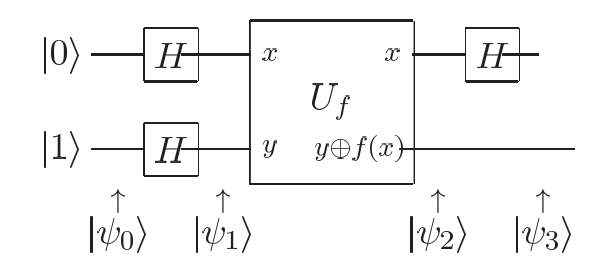
\includegraphics[width=0.5\textwidth]{Immagine18.png} 
    \caption{Circuito quantistico che implementa l'algoritmo generale di Deutsch–Jozsa. Il filo con un simbolo '/' rappresenta un insieme di \( n \) qubit, secondo la notazione ingegneristica comune.}
    \label{Immagine18}
\end{figure}
I passi dell'algoritmo sono illustrati in Figura 1.20:
\begin{enumerate}
    \item \textbf{Stato iniziale} \\
    Si dispone di un registro di $n$ qubit (query register) e di un qubit di risposta (answer register). Si prepara lo stato
    
    \begin{equation}
    \ket{\psi_0}
    = \ket{0}^{\otimes n} \otimes \ket{1}.
    \end{equation}
    
    \item \textbf{Hadamard sui registri} \\
    Si applica $H^{\otimes n}$ al registro query e $H$ al registro risposta, ottenendo
    
    \begin{equation}
    \ket{\psi_1}
    = \left(\frac{1}{\sqrt{2^n}}\sum_{x\in\{0,1\}^n}\ket{x}\right)
      \otimes
      \left(\frac{\ket{0} - \ket{1}}{\sqrt{2}}\right).
    \end{equation}
    
    \item \textbf{Oracolo $U_f$} \\
    Si invoca il circuito quantistico $U_f\colon\ket{x,y}\mapsto\ket{x,y\oplus f(x)}$, producendo
    
    \begin{equation}
    \ket{\psi_2}
    = \frac{1}{\sqrt{2^n}}
      \sum_{x\in\{0,1\}^n}(-1)^{f(x)}\,\ket{x}
      \otimes
      \left(\frac{\ket{0} - \ket{1}}{\sqrt{2}}\right).
    \end{equation}
    
    \item \textbf{Seconda trasformata di Hadamard} \\
    Si riapplica $H^{\otimes n}$ al registro query. Per ogni $x\in\{0,1\}^n$,
    
    \begin{equation}
    H^{\otimes n}\ket{x}
    = \frac{1}{\sqrt{2^n}}
      \sum_{z\in\{0,1\}^n}(-1)^{x\cdot z}\,\ket{z},
    \end{equation}
    
    dove $x\cdot z=\sum_{i=1}^n x_i z_i \pmod{2}$. Dunque lo stato diventa
    
    \begin{equation}
    \ket{\psi_3}
    = \frac{1}{2^n}
      \sum_{z\in\{0,1\}^n}
      \left(\sum_{x}(-1)^{x\cdot z + f(x)}\right)\,\ket{z}
      \otimes
      \left(\frac{\ket{0} - \ket{1}}{\sqrt{2}}\right).
    \end{equation}
    
    \item \textbf{Misura del registro query} \\
    Si misura il registro di $n$ qubit.
    
    \begin{itemize}
        \item \textbf{Se $f$ è costante}, allora per $z=0^n$ la somma interna
        $\sum_x(-1)^{f(x)} = \pm 2^n$ produce ampiezza $\pm 1$ per $\ket{0^n}$, e tutte le altre ampiezze sono nulle. La misura restituisce quindi $0^n$ con certezza.
        
        \item \textbf{Se $f$ è bilanciato}, i termini positivi e negativi si cancellano in corrispondenza di $z=0^n$, lasciando ampiezza zero; pertanto la misura dà un risultato diverso da $0^n$ con probabilità unitaria.
    \end{itemize}
\end{enumerate}
In tal modo, mediante una \textbf{singola} interrogazione dell'oracolo $U_f$, l'algoritmo distingue con esattezza le due classi di funzioni, ottenendo un vantaggio \textbf{esponenziale} rispetto al miglior algoritmo deterministico classico, che richiede $2^{n-1}+1$ interrogazioni.
\subsection*{Riassunto dell'algoritmo Deutsch--Jozsa}
\textbf{Problema (Deutsch--Jozsa).}
Sia dato un oracolo quantistico $U_f$ che realizza la trasformazione
\[
U_f\colon \ket{x}\ket{y} \longmapsto \ket{x}\ket{y \oplus f(x)},
\]
con $x\in\{0,\dots,2^n-1\}$ e $f(x)\in\{0,1\}$. È assicurato che $f$ sia \textbf{costante} (stesso valore per ogni $x$) oppure \textbf{bilanciata} (vale 1 per esattamente metà degli $x$ e 0 per l'altra metà).
\textbf{Obiettivo.}
Determinare con certezza se $f$ è costante o bilanciata.
\vspace{0.5em}\hrule\vspace{0.5em}
\subsubsection*{Algoritmo: Deutsch--Jozsa}
\begin{itemize}
    \item \textbf{Input:}
    \begin{itemize}
        \item Un oracolo $U_f$ come sopra.
    \end{itemize}
    
    \item \textbf{Output:}
    \begin{itemize}
        \item $0$ se e solo se $f$ è costante;
        \item un valore diverso da $0$ (ossia almeno un bit pari a 1) se e solo se $f$ è bilanciata.
    \end{itemize}
    
    \item \textbf{Complessità in tempo:}
    \begin{itemize}
        \item \textbf{Un'unica} applicazione dell'oracolo $U_f$.
    \end{itemize}
\end{itemize}
\subsubsection*{Procedura}
\begin{enumerate}
    \item \textbf{Inizializzazione} \\
    Prepara il registro di query e il registro di risposta nello stato
    
    \[
    \ket{\psi_0} = \ket{0}^{\otimes n} \otimes \ket{1}.
    \]
    
    \item \textbf{Creazione della sovrapposizione} \\
    Applica $H^{\otimes n}$ al registro di query e $H$ al registro di risposta:
    
    \[
    \ket{\psi_1}
    = \left(\frac{1}{\sqrt{2^n}}\sum_{x=0}^{2^n-1}\ket{x}\right)
      \otimes
      \left(\frac{\ket{0} - \ket{1}}{\sqrt{2}}\right).
    \]
    
    \item \textbf{Valutazione quantistica} \\
    Invoca l'oracolo:
    
    \[
    \ket{\psi_2}
    = U_f\ket{\psi_1}
    = \frac{1}{\sqrt{2^n}}
      \sum_{x=0}^{2^n-1}(-1)^{f(x)}\ket{x}
      \otimes
      \left(\frac{\ket{0} - \ket{1}}{\sqrt{2}}\right).
    \]
    
    \item \textbf{Interferenza} \\
    Riapplica $H^{\otimes n}$ al registro di query:
    
    \[
    \ket{\psi_3}
    = \frac{1}{2^n}
      \sum_{z=0}^{2^n-1}
      \left(\sum_{x=0}^{2^n-1}(-1)^{x\cdot z + f(x)}\right)
      \ket{z}
      \;\otimes\;
      \left(\frac{\ket{0} - \ket{1}}{\sqrt{2}}\right).
    \]
    
    \item \textbf{Misura finale} \\
    Misura i $n$ qubit del registro di query:
    
    \begin{itemize}
        \item Se il risultato è $z=0^n$ (tutti zeri), allora \textbf{$f$ è costante};
        \item altrimenti, \textbf{$f$ è bilanciata}.
    \end{itemize}
\end{enumerate}
\vspace{0.5em}\hrule\vspace{0.5em}
\textbf{Correttezza.}
\begin{itemize}
    \item Nel caso \textbf{costante}, $\sum_x(-1)^{f(x)} = \pm 2^n$ $\Rightarrow$ ampiezza unitaria su $\ket{0^n}$ e zero su tutti gli altri $\ket{z}$.
    \item Nel caso \textbf{bilanciato}, le fasi positive e negative si cancellano esattamente per $z=0^n$, lasciando ampiezza nulla su $\ket{0^n}$, e misura dunque $\neq 0^n$.
\end{itemize}
\textbf{Prestazioni.}
Rispetto ai $2^{n-1}+1$ interrogazioni classiche deterministiche, l'algoritmo quantum richiede una \textbf{singola} chiamata a $U_f$, mostrando un esempio di accelerazione esponenziale in un problema di natura oracolare.
\vspace{0.5em}\hrule\vspace{0.5em}
\noindent Pur essendo il problema di per sé privo di applicazioni pratiche dirette, l'algoritmo di Deutsch--Jozsa introduce i principi di \textbf{interferenza controllata} e \textbf{estrazione di informazione globale} da sovrapposizioni, che costituiscono la base di successivi algoritmi quantistici più utili e di maggiore impatto.

\section{Algoritmo di ricerca quantistica (Grover)}
\subsection{L'oracolo}
Consideriamo un problema di \textbf{ricerca} su uno spazio di $N$ elementi, numerati da $0$ a $N-1$. Per semplicità supponiamo $N=2^n$, in modo da rappresentare ciascun indice $x$ con un registro di $n$ qubit. L'istanza del problema è determinata da una funzione booleana
\[
f\colon\{0,1\}^n \to \{0,1\},
\]
tale che esattamente $M$ degli $N$ possibili input sono soluzioni ($f(x)=1$) e gli altri $N-M$ non lo sono ($f(x)=0$). L'\textbf{oracolo} quantistico corrispondente è un'unitarià $O$ agita su $n+1$ qubit ed è definita dalla sua azione sugli stati base computazionali:
\begin{equation}
O\colon \ket{x}\ket{q} \longmapsto \ket{x}\ket{q \oplus f(x)},
\end{equation}
dove il secondo qubit $\ket{q}$ --- detto \textbf{oracle qubit} --- viene invertito se e solo se $x$ è una soluzione ($f(x)=1$).
Nel \textbf{ricerca quantistica} si fa convenzionalmente agire l'oracolo su uno stato $\ket{x}$ tensore con l'oracolo qubit inizializzato in
\[
\frac{\ket{0} - \ket{1}}{\sqrt{2}}.
\]
In tal modo:
\begin{itemize}
    \item Se $f(x)=0$, il secondo qubit resta $\bigl(\ket{0} - \ket{1}\bigr)/\sqrt{2}$.
    \item Se $f(x)=1$, l'azione di $O$ produce un segno negativo, ossia
    
    \[
      \ket{x} \frac{\ket{0} - \ket{1}}{\sqrt{2}}
      \;\mapsto\;
      -\,\ket{x}\,\frac{\ket{0} - \ket{1}}{\sqrt{2}}.
    \]
\end{itemize}
Poiché lo stato del secondo qubit rimane invariato, esso può essere omesso dalla trattazione, e si scrive semplicemente
\begin{equation}
O\colon \ket{x} \longmapsto (-1)^{f(x)}\ket{x}.
\end{equation}
In altre parole, l'oracolo \textbf{``segnala''} le soluzioni innalzando la loro fase di $\pi$.
Nell'algoritmo di Grover, per trovare una soluzione basta applicare l'oracolo \textbf{un numero di volte dell'ordine di} $\sqrt{N/M}$ all'interno di un'apposita iterazione di ``riflessione'' e ``inversione''. Ciò rappresenta un \textbf{quadratico} miglioramento rispetto alle $\Theta(N/M)$ interrogazioni necessarie nel caso classico.
\vspace{0.5em}\hrule\vspace{0.5em}
\noindent \textbf{Nota.} L'oracolo è considerato un ``cassetto nero'': \textbf{riconosce} le soluzioni ma non ne fornisce direttamente i valori. Ciò è sufficiente per il computo quantistico, analogamente a quanto accade nei protocolli di fattorizzazione quantistica (es. Shor), in cui l'oracolo permette di \textbf{verificare} se un candidato è fattore primo, ma non di \textbf{generarlo} direttamente.
Affinché l'algoritmo quantistico di ricerca sia effettivamente utilizzabile, è necessario costruire un circuito quantistico efficiente che implementi l'oracolo. La realizzazione di tale circuito rappresenta un esercizio nelle tecniche di computazione reversibile.
Definiamo innanzitutto la funzione $f(x)$ come segue:
\[
f(x) = 
\begin{cases}
1 & \text{se } x \mid m  \quad (x \text{ divide } m), \\
0 & \text{altrimenti}.
\end{cases}
\]
Questa funzione restituisce $1$ se la divisione $m \div x$ ha resto nullo, ovvero se $x$ è un divisore esatto di $m$, e $0$ altrimenti. In altri termini, $f(x)$ indica se la divisione di prova ha successo oppure no.
Utilizzando le tecniche di computazione reversibile, è possibile costruire un circuito classico reversibile che agisca sulla coppia di registri $(x, q)$, dove $x$ rappresenta il registro di input inizializzato a un determinato valore e $q$ è un registro di uscita ad un bit, inizialmente impostato a $0$. Il circuito esegue la trasformazione
\[
(x, q) \rightarrow (x, q \oplus f(x)),
\]
modificando un circuito classico irreversibile standard per la divisione di prova in una versione reversibile.
Il costo in termini di risorse del circuito reversibile così ottenuto è, al più, il doppio di quello richiesto dal circuito classico irreversibile per la stessa operazione. Pertanto, possiamo considerare i due circuiti sostanzialmente equivalenti in termini di complessità computazionale.
Inoltre, il circuito classico reversibile può essere immediatamente tradotto in un circuito quantistico che realizza la trasformazione unitaria
\[
\ket{x}\ket{q} \rightarrow \ket{x}\ket{q \oplus f(x)},
\]
come richiesto dall'oracolo. Un aspetto fondamentale è che, pur non conoscendo i fattori primi di $m$, è comunque possibile costruire esplicitamente un oracolo che riconosca una soluzione al problema di ricerca, qualora essa si presenti.
Utilizzando tale oracolo in combinazione con l'algoritmo quantistico di ricerca, è possibile eseguire una ricerca nello spazio degli input compreso tra $2$ e $\lfloor \sqrt{m} \rfloor$ con un numero di interrogazioni dell'oracolo pari a $O(m^{1/4})$. Ciò implica che il numero di divisioni necessarie è ridotto da circa $\sqrt{m}$, come richiesto da un algoritmo classico basato su ricerca esaustiva, a $O(m^{1/4})$ nel caso quantistico.
Sebbene l'esempio della fattorizzazione sia concettualmente interessante, non risulta pratico nella realtà: esistono algoritmi classici per la fattorizzazione molto più efficienti rispetto alla semplice ricerca tra tutti i possibili divisori. Tuttavia, tale esempio illustra il principio generale secondo cui gli algoritmi classici basati su tecniche di ricerca possono beneficiare di un'accelerazione significativa mediante l'impiego dell'algoritmo quantistico di ricerca.
Nel prosieguo del capitolo verranno analizzati scenari nei quali l'algoritmo di ricerca quantistico può offrire un contributo realmente utile nell'accelerare la risoluzione di problemi NP-completi.
L'algoritmo opera schematicamente come illustrato nella Figura 6.1. Il nucleo dell'algoritmo utilizza un unico registro quantistico di $n$ qubit. I dettagli interni dell'oracolo $O$, inclusa l'eventuale necessità di qubit aggiuntivi, non sono rilevanti per la descrizione dell'algoritmo stesso. L'obiettivo è trovare una soluzione al problema di ricerca minimizzando il numero di applicazioni dell'oracolo.
\subsubsection{Inizializzazione}
L'algoritmo inizia con il computer nello stato $\ket{0}^{\otimes n}$. Una trasformata di Hadamard $H^{\otimes n}$ porta il sistema nella sovrapposizione uniforme:
\begin{equation}
\ket{\psi} = \frac{1}{\sqrt{N}}\sum_{x=0}^{N-1}\ket{x},
\end{equation}
dove $N = 2^n$.
\subsubsection{Iterazione di Grover}
L'algoritmo procede applicando ripetutamente un sottoblocco quantistico, detto \textbf{iterazione di Grover} (o operatore di Grover), denotato con $G$. La struttura del circuito quantistico è mostrata in Figura 6.2. Ogni iterazione $G$ si articola in quattro fasi:
\begin{enumerate}
    \item \textbf{Applicazione dell'oracolo $O$}: \\
    L'oracolo introduce uno sfasamento selettivo sugli stati soluzione.
    
    \item \textbf{Applicazione della trasformata di Hadamard $H^{\otimes n}$}: \\
    Trasforma lo stato nella base computazionale.
    
    \item \textbf{Sfasamento condizionale}: \\
    Viene applicato uno sfasamento di $-1$ a tutti gli stati della base computazionale eccetto $\ket{0}$:
    \[
    \ket{x} \to -(-1)^{\delta_{x0}} \ket{x}.
    \]
    
    \item \textbf{Ri-applicazione della trasformata di Hadamard $H^{\otimes n}$}.
\end{enumerate}
\subsubsection{Implementazione ed efficienza}
Tutte le operazioni nell'iterazione di Grover sono efficientemente implementabili:
\begin{itemize}
    \item I passi 2 e 4 (Hadamard) richiedono ciascuno $O(n)$ operazioni (poiché $n = \log_2 N$)
    \item Il passo 3 (sfasamento condizionale) è implementabile con $O(n)$ porte logiche,
    \item Il passo 1 (oracolo) richiede un'unica chiamata per iterazione; il suo costo dipende dall'applicazione specifica
\end{itemize}
\subsubsection{Analisi dell'iterazione di Grover}
L'effetto combinato dei passi 2, 3 e 4 equivale a:
\begin{equation}
H^{\otimes n} (2\ket{0}\bra{0} - I) H^{\otimes n} = 2\ket{\psi}\bra{\psi} - I,
\end{equation}
dove $\ket{\psi}$ è lo stato di sovrapposizione uniforme definito in (6.4). Pertanto, l'operatore di Grover assume la forma compatta:
\begin{equation}
G = (2\ket{\psi}\bra{\psi} - I)O.
\end{equation}
\subsubsection{Note formali}
\begin{itemize}
    \item \textbf{Correttezza dello sfasamento (Passo 3)}: \\
    L'espressione $\ket{x} \to -(-1)^{\delta_{x0}} \ket{x}$ è equivalente a:
    \begin{align*}
        \ket{0} &\mapsto \ket{0} \quad \text{(nessun sfasamento)} \\
        \ket{x} &\mapsto -\ket{x} \quad \text{per } x \neq 0 \quad \text{(sfasamento di $\pi$)}
    \end{align*}
    Ciò realizza la trasformazione unitaria $(2\ket{0}\bra{0} - I)$.
    
    \item \textbf{Ottimizzazione}: \\
    La formulazione $G = (2\ket{\psi}\bra{\psi} - I)O$ evidenzia il ruolo dell'\emph{inversione attorno alla media} (termine $2\ket{\psi}\bra{\psi} - I$) e dell'oracolo $O$.
    
    \item \textbf{Complessità}: \\
    L'implementazione complessiva di $G$ richiede $O(n)$ porte logiche, escludendo il costo dell'oracolo.
\end{itemize}
\begin{figure}[H]
    \centering
    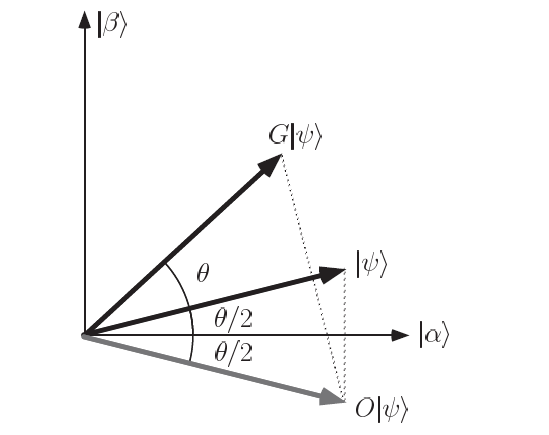
\includegraphics[width=0.5\textwidth]{Immagine19.png} 
    \caption{L'azione di una singola iterazione di Grover, \( G \): il vettore di stato viene ruotato di un angolo \( \theta \) verso la sovrapposizione \( \lvert \beta \rangle \) di tutte le soluzioni del problema di ricerca. Inizialmente, esso è inclinato di un angolo \( \theta/2 \) rispetto a \( \lvert \alpha \rangle \), uno stato ortogonale a \( \lvert \beta \rangle \). Un'operazione oracolare \( O \) riflette lo stato rispetto allo stato \( \lvert \alpha \rangle \), quindi l'operazione \( 2 \lvert \psi \rangle \langle \psi \rvert - I \) lo riflette rispetto a \( \lvert \psi \rangle \). Nella figura, \( \lvert \alpha \rangle \) e \( \lvert \beta \rangle \) sono leggermente allungati per ridurre la confusione (tutti gli stati dovrebbero comunque essere vettori unitari). Dopo ripetute iterazioni di Grover, il vettore di stato si avvicina a \( \lvert \beta \rangle \), momento in cui una misurazione nella base computazionale restituisce con alta probabilità una soluzione al problema di ricerca. L'efficienza notevole dell'algoritmo si deve al fatto che \( \theta \) si comporta come \( \Omega(\sqrt{M/N}) \), quindi sono necessarie solo \( \mathcal{O}(\sqrt{N/M}) \) applicazioni di \( G \) per ruotare il vettore di stato vicino a \( \lvert \beta \rangle \).}
    \label{Immagine19}
\end{figure}

\section{Algoritmo di Shor (cenni)}
\subsection{Introduzione}
L'algoritmo di Shor, proposto da Peter Shor nel 1994, rappresenta una pietra miliare nell'informatica quantistica. Esso risolve efficientemente il problema della \textbf{fattorizzazione di interi}, computazionalmente intrattabile per computer classici. La rilevanza crittografica risiede nella capacità di violare il sistema RSA, fondato sulla difficoltà di fattorizzare grandi semiprimi.

\subsection{Problema della Fattorizzazione}
Dato un intero composto \(N\) (semiprimo \(N = pq\), dove \(p\) e \(q\) sono primi distinti), il problema consiste nel determinare \(p\) e \(q\). I migliori algoritmi classici (es. \textit{General Number Field Sieve}) richiedono tempo subesponenziale \(O\left(\exp\left[(\log N)^{1/3}(\log \log N)^{2/3}\right]\right)\), rendendo il problema intrattabile per chiavi RSA grandi.

\subsection{Struttura dell'Algoritmo}
L'algoritmo combina elementi classici e quantistici:

\begin{enumerate}
    \item \textbf{Parte Classica}: Riduzione a un problema di ricerca d'ordine
    \item \textbf{Parte Quantistica}: Soluzione del problema d'ordine
    \item \textbf{Parte Classica}: Estrazione dei fattori
\end{enumerate}

\subsection{Riduzione Classica a Ricerca d'Ordine}
Scegliere casualmente \(a \in \{2, \dots, N-1\}\) con \(\gcd(a, N) = 1\). L'\textbf{ordine} di \(a\) modulo \(N\) è il minimo \(r\) tale che:
\[
a^r \equiv 1 \pmod{N}.
\]
Se \(r\) è pari e \(a^{r/2} \not\equiv -1 \pmod{N}\), allora \(\gcd(a^{r/2} \pm 1, N)\) fornisce un fattore non banale con probabilità \(\geq \frac{1}{2}\).

\subsection{Subroutine Quantistica: Ricerca d'Ordine}
Il cuore quantistico utilizza la \textbf{stima di fase} su un operatore unitario speciale.

\subsubsection{Operatore Modulare}
Definiamo l'operatore \(U\) su \(\mathscr{H} = \mathbb{C}^L \otimes \mathbb{C}^L\) (\(L = \lceil \log_2 N \rceil\)):
\[
U|y\rangle = |a y \mod N\rangle, \quad y \in \{0,1\}^L.
\]
I suoi autostati sono:
\[
|u_s\rangle = \frac{1}{\sqrt{r}} \sum_{k=0}^{r-1} \exp\left(-\frac{2\pi i s k}{r}\right) |a^k \mod N\rangle
\]
con autovalori \(\exp(2\pi i s / r)\).

\subsubsection{Circuit Quantistico}
\begin{figure}[h]
    \centering
    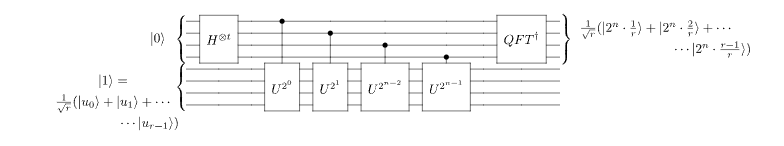
\includegraphics[width=1\textwidth]{Immagine21.png}
    \caption{Schema del circuito quantistico per la ricerca d'ordine}
    \label{fig:shor}
\end{figure}

Il circuito (Fig. \ref{fig:shor}) opera su due registri:
\begin{itemize}
    \item \textit{Registro di controllo}: \(t = 2L + 1 + \lceil \log(2 + 1/(2\epsilon)) \rceil\) qubit
    \item \textit{Registro di lavoro}: \(L\) qubit inizializzati a \(|1\rangle\)
\end{itemize}

\subsubsection{Fasi Quantistiche}
\begin{enumerate}
    \item \textbf{Inizializzazione}: 
    \[
    |\psi_0\rangle = |0\rangle^{\otimes t} \otimes |1\rangle
    \]
    
    \item \textbf{Applicazione Hadamard}:
    \[
    |\psi_1\rangle = \frac{1}{\sqrt{2^t}} \sum_{j=0}^{2^t-1} |j\rangle \otimes |1\rangle
    \]
    
    \item \textbf{Esponenziazione Modulare}:
    \[
    |\psi_2\rangle = \frac{1}{\sqrt{2^t}} \sum_{j=0}^{2^t-1} |j\rangle \otimes |a^j \mod N\rangle
    \]
    
    \item \textbf{Trasformata di Fourier Quantistica}:
    \[
    |\psi_3\rangle = \text{QFT}_t^{\dagger} |\psi_2\rangle = \sum_{k=0}^{2^t-1} \alpha_k |k\rangle \otimes |a^j \mod N\rangle
    \]
    
    \item \textbf{Misurazione}: Si misura il registro di controllo ottenendo un valore \(c \approx \frac{s}{r} \cdot 2^t\).
\end{enumerate}

\subsection{Estrazione dell'Ordine}
Dalla misura \(c\), si ottiene l'approssimazione \(\phi \approx s/r\). Con l'algoritmo delle \textbf{frazioni continue}, si ricava \(r\):
\[
\left| \frac{c}{2^t} - \frac{s}{r} \right| \leq \frac{1}{2^{t+1}}.
\]
La probabilità di successo per ogni \(s\) è \(\geq (1-\epsilon)/r\).

\subsection{Complessità Computazionale}
\begin{itemize}
    \item \textbf{Esponenziazione modulare}: \(O(L^3)\) operazioni
    \item \textbf{QFT}: \(O(L^2)\) operazioni
    \item \textbf{Iterazioni}: \(O(1)\) (probabilità costante)
\end{itemize}
Complessità totale: \(O(L^3) = O((\log N)^3)\), esponenzialmente più efficiente dei metodi classici.

\subsection{Analisi di Correttezza}
\begin{theorem}[Shor 1994]
Per ogni \(\epsilon > 0\), l'algoritmo restituisce un fattore non banale di \(N\) con probabilità \(\Omega(1)\) in tempo \(O((\log N)^3 \log \log N)\).
\end{theorem}
La dimostrazione poggia su:
\begin{itemize}
    \item Teoria dei numeri per la riduzione
    \item Proprietà della QFT per la stima
    \item Analisi delle frazioni continue per l'estrazione di \(r\)
\end{itemize}

\subsection{Conclusioni}
L'algoritmo di Shor dimostra la potenza teorica del calcolo quantistico, risolvendo efficientemente un problema ritenuto intrattabile classicamente. Le sue implicazioni crittografiche hanno stimolato lo sviluppo della \textbf{post-quantum cryptography}. Implementazioni pratiche richiedono correzione d'errore quantistica, attualmente area di ricerca attiva.

\chapter{Simulazione e software}
La simulazione quantistica rappresenta una metodologia fondamentale per investigare sistemi fisici complessi dove i calcoli classici diventano intrattabili. Secondo il paradigma introdotto da Feynman nel 1982, un computer quantistico può emulare efficientemente l'evoluzione temporale di altri sistemi quantistici, superando le limitazioni degli approcci computazionali tradizionali. Questo principio trova applicazione in campi multidisciplinari quali la chimica computazionale, la scienza dei materiali e la fisica delle alte energie.

\section{Architettura Software per Simulatori Quantistici}
I moderni software per simulazione quantistica si strutturano su più livelli funzionali:
\begin{equation}
\Pi_{\text{sim}} = \mathcal{C}_{\text{controllo}} \otimes \Lambda_{\text{backend}} \oplus \Gamma_{\text{visualizzazione}}
\end{equation}
dove $\mathcal{C}_{\text{controllo}}$ gestisce l'astrazione del circuito quantistico, $\Lambda_{\text{backend}}$ implementa il motore di simulazione vero e proprio, e $\Gamma_{\text{visualizzazione}}$ fornisce strumenti diagnostici. 

\vspace{0.2cm}
\noindent Le piattaforme più evolute implementano:
\begin{enumerate}
    \item \textbf{Compilazione ottimizzata}: Trasformazione di circuiti mediante equivalenze algebriche (es. identità di ZX-calculus)
    \item \textbf{Simulazione ibrida}: Integrazione tra componenti classiche e quantistiche (modello QRAM)
    \item \textbf{Calcolo simbolico}: Manipolazione di operatori tramite algebra di Lie (pacchetti come \texttt{OpenFermion})
\end{enumerate}

\subsection{Benchmark delle Piattaforme}
La Tabella~\ref{tab:software_quantistici} confronta le capacità di simulazione di framework principali:
\begin{table}[h]
\centering
\caption{Caratteristiche di software per simulazione quantistica}
\label{tab:software_quantistici}
\begin{tabular}{|l|c|c|c|}
\hline
\textbf{Software} & \textbf{Qubit simulati} & \textbf{Gate set} & \textbf{Backend} \\ \hline
Qiskit & $\sim 10^3$ (stato vett.) & Universale & CPU/GPU \\ 
Cirq & $\sim 10^4$ (tensore) & Personalizzabile & TPU \\
ProjectQ & $\sim 10^2$ & Ad alto livello & HPC \\ \hline
\end{tabular}
\end{table}

\noindent Le limitazioni principali risiedono nella complessità spaziale: la rappresentazione dello stato quantistico richiede $\mathcal{O}(2^n)$ risorse classiche. Tecniche avanzate come la \textit{stabilizer simulation} o i \textit{tensor network} mitigano questo problema per specifiche classi di circuiti.

\subsection{Applicazioni Pratiche}
In ambito accademico-industriale, questi strumenti abilitano:
\begin{itemize}
    \item Progettazione di nuovi farmaci mediante simulazione di dinamica molecolare
    \item Ottimizzazione di materiali superconduttori
    \item Analisi di stati quantistici topologici
\end{itemize}
La sfida contemporanea risiede nello sviluppo di API unificate che permettano la portabilità degli algoritmi tra simulatori software e hardware quantistico reale, obiettivo perseguito da iniziative come QIR.
\subsection{Algoritmi Ibridi Quantistico-Classici}
\label{subsec:algoritmi-ibridi}

La simulazione quantistica riveste un ruolo cruciale nello sviluppo e validazione di algoritmi ibridi, in particolare per il variational quantum eigensolver (VQE) e il quantum approximate optimization algorithm (QAOA). Questi protocolli sfruttano sinergie tra:
\begin{equation}
\mathcal{H}_{\text{ibrido}} = \underbrace{\sum_k \theta_k U_k(\vec{\phi})}_{\text{ansatz quantistico}} + \underbrace{\mathcal{O}(\rho_{\text{classico}})}_{\text{ottimizzatore}}
\end{equation}
dove il ciclo di ottimizzazione classica aggiorna iterativamente i parametri $\theta_k$ basandosi sull'output dei simulatori. Framework come \texttt{TensorFlow Quantum} implementano gradienti automatici mediante la regola di parametri shift:
\begin{equation}
\nabla_\theta \langle \psi(\theta) | H | \psi(\theta) \rangle = \frac{1}{2} \left[ \langle H \rangle_{\theta + \pi/2} - \langle H \rangle_{\theta - \pi/2} \right]
\end{equation}

\subsection{Modellazione del Rumore e Mitigazione degli Errori}
\label{subsec:rumore}

Per avvicinare le simulazioni alle condizioni sperimentali, i software moderni integrano modelli di rumore realistici:
\begin{itemize}
    \item \textbf{Modelli di canale quantistico}: Rappresentati tramite matrici di Pauli-twirl $\mathcal{E}(\rho) = \sum_k E_k \rho E_k^\dagger$
    \item \textbf{Errori correlati}: Simulazione di cross-talk e errori spazialmente correlati
    \item \textbf{Teoria dell'informazione quantistica}: Calcolo dell'entanglement fidelity $F_e = \langle \phi | \mathcal{E}(|\phi\rangle\langle\phi|) | \phi \rangle$
\end{itemize}
Le tecniche di mitigazione avanzate includono:
\begin{enumerate}
    \item Zero-noise extrapolation (ZNE) mediante stretching temporale
    \item Probabilistic error cancellation (PEC) con quasiprobabilità
    \item Clifford data regression (CDR) per stati non stabilizzanti
\end{enumerate}

\subsection{Parallelizzazione e Tecniche di Compressione}
\label{subsec:parallelizzazione}

Per superare i limiti computazionali, i simulatori adottano strategie avanzate:
\begin{table}[h]
\centering
\caption{Tecniche di efficientamento computazionale}
\label{tab:tecniche-efficientamento}
\begin{tabular}{p{0.25\textwidth}p{0.7\textwidth}}
\toprule
\textbf{Tecnica} & \textbf{Implementazione} \\
\midrule
State vector parallelization & Distribuzione MPI su cluster HPC con schemi di comunicazione a bassa latenza \\
Tensor network contraction & Ottimizzazione dell'ordine di contrazione mediante algoritmi di tree decomposition \\
Stochastic methods & Metodi Monte Carlo quantistico (es. walkers stocastici per fermioni) \\
Symmetry exploitation & Riduzione della base di Hilbert sfruttando i numeri quantici conservati \\
\bottomrule
\end{tabular}
\end{table}

\noindent Recenti sviluppi nel calcolo simbolico permettono la manipolazione di hamiltoniane complesse tramite algebra di Jordan-Wigner e trasformazioni di Bravyi-Kitaev, riducendo la complessità da $\mathcal{O}(N^4)$ a $\mathcal{O}(N^2)$ per sistemi elettronici.

\subsection{Sfide Future e Sviluppi}
\label{subsec:sfide}

Nonostante i progressi, permangono sfide significative:
\begin{itemize}
    \item \textbf{Complessità temporale}: La simulazione di dinamiche quantistiche generali rimane \#P-difficile
    \item \textbf{Verifica e validazione}: Problema della certificazione per stati a grande entanglement
    \item \textbf{Interoperabilità}: Necessità di standard per lo scambio di stati quantistici (formati QASM, Quil)
\end{itemize}
Le roadmap di sviluppo puntano su:
\begin{itemize}
    \item Integrazione con intelligenza artificiale (reti neurali quantistiche)
    \item Simulatori specializzati per hardware specifici (superconduttori, trappole ioniche)
    \item Metodi tensor-free basati su quantum state diffusion
\end{itemize}
L'emergere di quantum processing units (QPUs) cloud-accessible richiederà una ricalibrazione dei simulatori, sempre più orientati a funzionare come validator per hardware reale piuttosto che mere piattaforme di calcolo.
Queste ultime cose verranno discusse in seguito nel capitolo 7.
\section{Introduzione al Framework Cirq}
\label{sec:cirq-intro}

Cirq è una libreria open-source sviluppata da Google Quantum AI per la creazione, manipolazione e simulazione di circuiti quantistici, con particolare attenzione all'hardware NISQ (Noisy Intermediate-Scale Quantum). Come discusso in precedenza, Cirq si colloca nella categoria dei simulatori tensoriali (Tabella~\ref{tab:software_quantistici}), distinguendosi per l'approccio hardware-aware che consente una modellazione fedele delle caratteristiche fisiche dei processori quantistici superconduttori.

\subsection{Filosofia Progettuale e Dominio di Applicazione}
\label{subsec:cirq-design}

La progettazione di Cirq segue tre principi fondamentali:
\begin{enumerate}
    \item \textbf{Device-aware}: Astrazione diretta delle topologie fisiche dei qubit (es. griglie 2D) e dei gate nativi
    \item \textbf{Algoritmi ibridi}: Integrazione nativa con TensorFlow per pipeline quantistico-classiche
    \item \textbf{Verifica sperimentale}: Strumenti per caratterizzare dispositivi reali mediante esperimenti di calibrazione
\end{enumerate}

L'architettura risponde alle sfide di simulazione delineate nella Sottosezione~\ref{subsec:sfide}, particolarmente per:
\begin{itemize}
    \item Prototipazione di algoritmi per processori Sycamore
    \item Simulazione di dinamiche a lungo range in chimica quantistica
    \\item Benchmarking di errori correlati (cfr. Sezione~\ref{subsec:rumore})
\end{itemize}

\subsection{Architettura del Framework}
\label{subsec:cirq-arch}

L'ecosistema Cirq si struttura in componenti modulari:
\begin{equation}
\mathsf{Cirq} = \mathcal{C}_{\mathtt{Core}} \oplus \mathcal{Q}_{\mathtt{Sim}} \oplus \mathcal{V}_{\mathtt{isualization}} \oplus \mathcal{I}_{\mathtt{on}}
\end{equation}

\noindent\textbf{Core Components}:
\begin{itemize}
    \item \texttt{Qubit}: Rappresentazione fisica con coordinate (es. \texttt{GridQubit(2,3)})
    \item \texttt{Moments}: Temporizzazione parallela delle operazioni
    \item \texttt{Gate}: Set estensibile di operazioni quantistiche
\end{itemize}

\noindent\textbf{Simulation Backends}:
\begin{itemize}
    \item \texttt{Simulator}: Simulatore vettoriale con supporto noise model
    \item \texttt{SimulatorT}: Implementazione tensoriale per circuiti a grande profondità
    \item \texttt{QuantumVirtualMachine}: Emulazione fedele di hardware specifico
\end{itemize}

\subsection{Modellazione Hardware-Aware}
\label{subsec:cirq-hardware}

La rappresentazione dei vincoli hardware è realizzata attraverso:
\begin{lstlisting}[language=Python,caption=Esempio di dispositivo hardware-aware in Cirq]
device = cirq.GridDevice(
    qubits = [cirq.GridQubit(i,j) for i in range(3) for j in range(3)],
    gate_duration = {(cirq.CZ): 25e-9, (cirq.PhasedXZGate): 15e-9},
    topology = cirq.Topology(qubit_pairs=[((0,0),(0,1)), ...])
)
\end{lstlisting}

Questa modellazione consente:
\begin{itemize}
    \item Validazione di circuiti rispetto ai vincoli fisici
    \item Stima realistica dei tempi di esecuzione
    \item Generazione automatica di sequenze di compilazione
\end{itemize}

\subsection{Integrazione con Algoritmi Ibridi}
\label{subsec:cirq-hybrid}

Per gli algoritmi ibridi menzionati nella Sottosezione~\ref{subsec:algoritmi-ibridi}, Cirq fornisce:
\begin{itemize}
    \item \texttt{cirq.TrialResult}: Struttura per gestire risultati parametrici
    \item \texttt{cirq.optimizers}: Ottimizzatori per VQE/QAOA (es. Powell, Nelder-Mead)
    \item \texttt{cirq.google.QuantumEngine}: Interfaccia a QPU cloud
\end{itemize}

L'integrazione con TensorFlow Quantum permette:
\begin{equation}
\min_{\vec{\theta}} \underbrace{\text{tfq.layers.Expectation}( \underbrace{\text{cirq.Circuit}}_{\text{ansatz}}, \underbrace{H}_{\text{hamiltoniana}} )}_{\text{loss function}} + \lambda \mathcal{R}(\vec{\theta})
\end{equation}

\subsection{Simulazione del Rumore}
\label{subsec:cirq-noise}

Implementando i modelli della Sottosezione~\ref{subsec:rumore}, Cirq supporta:
\begin{itemize}
    \item Canali quantistici personalizzabili (Kraus operators)
    \item Errori correlati spazialmente e temporalmente
    \item Metodi di mitigazione avanzati:
\end{itemize}

\begin{lstlisting}[language=Python]
noise_model = cirq.NoiseModel.from_calibration(
    calibration_data, 
    error_functions={
        cirq.DepolarizingChannel: _depol_error,
        cirq.AmplitudeDampingChannel: _amp_damp_error
    }
)
simulator = cirq.DensityMatrixSimulator(noise=noise_model)
\end{lstlisting}

\subsection{Performance e Benchmark}
\label{subsec:cirq-bench}

Le capacità computazionali di Cirq sono ottimizzate per:
\begin{itemize}
    \item Simulazione di circuiti a 30+ qubit su GPU NVIDIA
    \item Parallelizzazione MPI tramite \texttt{cirq.SimulatorBase}
    \item Contrazione efficiente di tensor network con backend XLA
\end{itemize}

\begin{table}[h]
\centering
\caption{Benchmark comparativo su simulazione Hamiltonian ground state (8 qubit)}
\label{tab:cirq-benchmark}
\begin{tabular}{lccc}
\toprule
\textbf{Framework} & \textbf{Tempo (s)} & \textbf{Memoria (GB)} & \textbf{Accuracy} \\
\midrule
Cirq (CPU) & 42.3 & 8.1 & 0.998 \\
Cirq (GPU) & 6.7 & 8.5 & 0.998 \\
Qiskit & 89.1 & 12.3 & 0.992 \\
ProjectQ & 121.4 & 9.8 & 0.997 \\
\bottomrule
\end{tabular}
\end{table}

\subsection{Estensioni Specialistiche}
\label{subsec:cirq-extensions}

La flessibilità di Cirq supporta domini applicativi avanzati:
\begin{itemize}
    \item \texttt{cirq-ft}: Operatori per computazione fault-tolerant
    \item \texttt{cirq-pasqal}: Estensioni per trappole ioniche
    \item \texttt{cirq-google}: Protocolli specifici per processori Google
    \item \texttt{OpenFermion-Cirq}: Chimica quantistica
\end{itemize}

\subsection{Workflow Tipico di Ricerca}
\label{subsec:cirq-workflow}

Un flusso di lavoro accademico con Cirq segue tipicamente:
\begin{enumerate}
    \item Definizione dell'hardware target (reale o simulato)
    \item Sintesi del circuito con gate nativi
    \item Iniezione di modelli di rumore realistici
    \item Simulazione con backends specializzati (stato vettore o densità)
    \item Validazione mediante metriche quantistiche (fidelity, entanglement entropy)
    \item Esecuzione ibrida su QPU cloud con correzione errori
\end{enumerate}

\subsection{Limitazioni e Sviluppi Futuri}
\label{subsec:cirq-future}

Sebbene Cirq rappresenti lo stato dell'arte, permangono sfide:
\begin{itemize}
    \item Supporto limitato per errori non-Markoviani
    \item Ottimizzazioni per architetture non-grid
    \item Integrazione con linguaggi di specifica formale
\end{itemize}

Le roadmap di sviluppo includono:
\begin{itemize}
    \item Compilatori basati su ZX-calculus
    \item Simulatori tensor-free per dinamica quantistica
    \item Interfacce unificate per quantum control
\end{itemize}
\section{Definizione e simulazione di circuiti}

Nel contesto del calcolo quantistico, i circuiti quantistici rappresentano il modello computazionale predominante. Essi costituiscono l'equivalente quantistico dei circuiti logici classici e permettono l'esecuzione di algoritmi sfruttando le proprietà distintive della meccanica quantistica, quali la sovrapposizione e l'entanglement. Un circuito quantistico può essere formalmente definito come una sequenza ordinata di operazioni (gate quantistici) applicate a un insieme di qubit, dove ciascuna operazione corrisponde a una trasformazione unitaria.

\subsection{Formalismo matematico dei circuiti quantistici}

Nel formalismo del circuito, uno stato quantistico iniziale $\ket{\psi_0}$ subisce una serie di trasformazioni unitarie $U_1, U_2, \dots, U_n$, ciascuna delle quali rappresenta una porta quantistica. Lo stato finale $\ket{\psi_f}$ del sistema sarà dato da:

\[
\ket{\psi_f} = U_n \cdots U_2 U_1 \ket{\psi_0}
\]

Ogni porta quantistica agisce su uno o più qubit, e le più comuni includono:

\begin{itemize}
  \item \textbf{Porta Hadamard ($H$)}: crea una sovrapposizione equa tra gli stati base.
  \item \textbf{Porta Pauli ($X$, $Y$, $Z$)}: operazioni analoghe a NOT, rotazioni sull'asse $x$, $y$ e $z$.
  \item \textbf{Porta di fase ($S$, $T$)}: introducono fasi complesse negli stati.
  \item \textbf{Porta CNOT (Controlled-NOT)}: introduce entanglement tra qubit.
\end{itemize}

Il circuito viene rappresentato graficamente su un diagramma, in cui i qubit sono linee orizzontali e le porte sono applicate da sinistra a destra.

\subsection{Struttura di un circuito quantistico}

Un circuito quantistico si compone di tre fasi principali:

\begin{enumerate}
  \item \textbf{Inizializzazione}: ogni qubit è inizializzato nello stato $\ket{0}$, salvo diversa specifica.
  \item \textbf{Evoluzione unitaria}: applicazione di una sequenza di gate secondo la logica dell’algoritmo.
  \item \textbf{Misurazione}: proiezione dello stato quantistico su uno degli stati base del sistema.
\end{enumerate}

A differenza dei circuiti classici, le operazioni quantistiche devono essere reversibili e descritte da matrici unitarie. La misurazione, tuttavia, è una trasformazione non unitaria, in quanto collassa lo stato quantistico in un'autostato dell'osservabile misurata.

\subsection{Simulazione software di circuiti quantistici}

La progettazione e verifica di circuiti quantistici reali è ancora un compito complesso a causa della fragilità dei qubit fisici. Per questo motivo, si fa largo uso di simulatori software che permettono di modellare circuiti e osservarne il comportamento teorico.

Tra gli strumenti più diffusi si annoverano:

\begin{itemize}
  \item \textbf{Qiskit} (IBM): framework open-source in Python, permette la definizione, esecuzione e visualizzazione di circuiti quantistici.
  \item \textbf{Cirq} (Google): focalizzato su circuiti a bassa profondità e vicini all'hardware NISQ.
  \item \textbf{QuTiP}: per simulazioni avanzate di sistemi quantistici aperti.
  \item \textbf{Q\#} (Microsoft): linguaggio di programmazione dedicato al calcolo quantistico, integrato con la Quantum Development Kit.
\end{itemize}

In questo elaborato si è scelto di utilizzare \textbf{Cirq}, in quanto si adatta bene all'obiettivo di costruire circuiti semplici per dimostrazioni teoriche e sperimentazioni didattiche.

\subsection{Costruzione e simulazione di un circuito con Cirq}

L'implementazione di un circuito in Cirq segue una logica modulare. Di seguito si mostra un esempio di circuito che prepara una sovrapposizione e introduce entanglement tra due qubit:

\begin{lstlisting}[language=Python, caption={Costruzione di un circuito in Cirq}]
import cirq

# Definizione dei qubit
q0, q1 = cirq.LineQubit.range(2)

# Definizione del circuito
circuit = cirq.Circuit()
circuit.append(cirq.H(q0))          # Sovrapposizione
circuit.append(cirq.CNOT(q0, q1))   # Entanglement

# Misurazione
circuit.append(cirq.measure(q0, q1, key='result'))

# Simulazione
simulator = cirq.Simulator()
result = simulator.run(circuit, repetitions=1000)
print(result.histogram(key='result'))
\end{lstlisting}

Questo circuito produce uno stato entangled di tipo Bell, in cui i due qubit risultano correlati in modo quantistico. L'output sarà una distribuzione binaria concentrata sugli stati $\ket{00}$ e $\ket{11}$.

\subsection{Ruolo della simulazione nel quantum computing}

La simulazione svolge un ruolo cruciale nell'attuale fase di sviluppo del calcolo quantistico. Essa consente:

\begin{itemize}
  \item La validazione teorica degli algoritmi prima dell'esecuzione su hardware reale.
  \item Lo studio di fenomeni come la decoerenza e la fedeltà delle operazioni.
  \item L'educazione e la formazione nei principi della meccanica quantistica computazionale.
\end{itemize}

Nonostante i limiti computazionali dovuti alla crescita esponenziale dello spazio di Hilbert con l'aumentare del numero di qubit, le simulazioni software restano uno strumento indispensabile per l'evoluzione della disciplina, in attesa della maturazione delle piattaforme hardware su larga scala.



\chapter{Error correction e fault tolerance}
\section{Concetti base di rumore quantistico}
Nella computazione quantistica, il rumore rappresenta uno degli ostacoli più critici alla realizzazione pratica di dispositivi affidabili e scalabili. A differenza dei sistemi classici, dove il rumore può essere spesso trascurabile o gestito mediante tecniche di ridondanza, i sistemi quantistici sono intrinsecamente sensibili all'ambiente, a causa del principio di decoerenza e della natura fragile degli stati quantistici.
\subsection{Decoerenza e disaccoppiamento}
La \textbf{decoerenza} è il processo mediante il quale un sistema quantistico perde le sue proprietà quantistiche a causa dell'interazione con l'ambiente circostante. In particolare, la sovrapposizione degli stati viene distrutta e il sistema tende verso una descrizione classica. Dal punto di vista matematico, questo fenomeno è descritto dalla perdita delle componenti fuori diagonale della matrice densità:
\[
\rho = \sum_{i,j} \rho_{ij} \ket{i}\bra{j} \quad \Rightarrow \quad \rho' = \sum_i \rho_{ii} \ket{i}\bra{i}
\]
dove $\rho_{ij}$ con $i \neq j$ sono le componenti responsabili delle interferenze quantistiche.
La decoerenza può essere provocata da vari meccanismi fisici, tra cui:
\begin{itemize}
  \item \textbf{Rumore termico}, dovuto alle vibrazioni dell'ambiente a temperatura diversa dallo zero assoluto.
  \item \textbf{Fluttuazioni del campo elettromagnetico}, che agiscono come perturbazioni esterne.
  \item \textbf{Interazioni incontrollate tra qubit}, che possono introdurre entanglement non desiderato con altri sottosistemi.
\end{itemize}
\subsection{Modelli di canali rumorosi}
Il rumore quantistico può essere modellato formalmente attraverso i cosiddetti \textit{canali quantistici}, che rappresentano mappe completamente positive e traccianti sullo spazio degli operatori di densità. Un canale quantistico $\mathcal{E}$ agisce su uno stato $\rho$ secondo:
\[
\mathcal{E}(\rho) = \sum_k E_k \rho E_k^\dagger
\]
dove gli operatori $\{E_k\}$, detti \textbf{operatori di Kraus}, soddisfano la condizione:
\[
\sum_k E_k^\dagger E_k = \mathbb{I}
\]
I modelli più comuni di canali rumorosi includono:
\begin{itemize}
  \item \textbf{Bit-flip}: simula un errore di tipo NOT con una certa probabilità $p$.
  \[
  \mathcal{E}(\rho) = (1-p)\rho + p X \rho X
  \]
  \item \textbf{Phase-flip}: simula un'inversione di fase, tramite l'operatore Pauli $Z$.
  \item \textbf{Depolarizing channel}: rappresenta una perdita completa di informazione quantistica.
  \[
  \mathcal{E}(\rho) = (1 - p) \rho + \frac{p}{3} (X\rho X + Y\rho Y + Z\rho Z)
  \]
  \item \textbf{Amplitude damping}: modello fisicamente realistico per la perdita di energia (es. emissione spontanea).
\end{itemize}
Tali canali sono fondamentali per comprendere come gli errori si propagano nei circuiti quantistici e per progettare tecniche correttive.
\subsection{Rumore nei simulatori software}
I simulatori quantistici moderni, come Qiskit e Cirq, consentono di modellare circuiti rumorosi per analizzare la robustezza degli algoritmi. Ad esempio, in Cirq è possibile definire un canale di depolarizzazione su un qubit come segue:
\begin{lstlisting}[language=Python, caption={Esempio di rumore depolarizzante in Cirq}]
import cirq

qubit = cirq.LineQubit(0)
circuit = cirq.Circuit()

# Applichiamo una porta Hadamard
circuit.append(cirq.H(qubit))

# Aggiungiamo un canale di rumore
circuit.append(cirq.depolarize(p=0.1)(qubit))

# Misuriamo il qubit
circuit.append(cirq.measure(qubit))

# Simulazione
sim = cirq.DensityMatrixSimulator()
result = sim.run(circuit, repetitions=1000)
print(result.histogram(key='0'))
\end{lstlisting}
La possibilità di introdurre modelli di rumore realistici nei simulatori permette di effettuare studi sistematici sull'impatto degli errori, oltre che di testare algoritmi di correzione degli stessi.
\subsection{Effetti del rumore sugli algoritmi quantistici}
Il rumore può compromettere significativamente le prestazioni degli algoritmi quantistici. In particolare:
\begin{itemize}
  \item \textbf{Riduzione della fedeltà}: lo stato risultante differisce da quello atteso.
  \item \textbf{Collasso precoce della coerenza}: le sovrapposizioni decadono prima della fine dell'algoritmo.
  \item \textbf{Errori di misura}: l'output misurato non corrisponde all'effettiva distribuzione teorica.
\end{itemize}
Per affrontare tali problemi, la ricerca si è concentrata sullo sviluppo di \textbf{codici di correzione quantistica} (Quantum Error Correction Codes, QECC), come il codice di Shor o quello di Steane, e sulla progettazione di architetture fault-tolerant.
\subsection{Prospettive e mitigazione}
Nel paradigma attuale dei dispositivi NISQ (Noisy Intermediate-Scale Quantum), in cui si dispone di un numero limitato di qubit e l'errore è ancora significativo, si fa affidamento a tecniche di \textbf{mitigazione del rumore}, che includono:

\begin{itemize}
  \item \textbf{Ripetizione statistica} e \textbf{media dei risultati}.
  \item \textbf{Calibrazione dinamica} dei gate e delle misurazioni.
  \item \textbf{Tecniche di compilazione ottimizzata} per minimizzare la profondità del circuito.
  \item \textbf{Estimatori robusti} per ridurre la varianza statistica dei risultati misurati.
\end{itemize}

In futuro, l'avanzamento delle tecnologie fisiche e delle tecniche di controllo quantistico potrà permettere la realizzazione di macchine quantistiche tolleranti al rumore, aprendo le porte a una computazione quantistica universale su larga scala.


\section{Il bit-flip code a 3 qubit}
Il bit-flip code a 3 qubit rappresenta uno dei primi e più semplici esempi di codice di correzione quantistica, storicamente introdotto per illustrare i principi fondamentali della correzione di errori quantistici. Questo codice è progettato specificamente per rilevare e correggere errori di tipo bit-flip, ovvero errori che invertono lo stato di un qubit da $\ket{0}$ a $\ket{1}$ e viceversa, analogamente al flip di un bit classico.
\subsection{Motivazione e contesto storico}
La necessità di sviluppare tecniche di correzione degli errori quantistici emerge dalla natura intrinsecamente fragile degli stati quantistici. A differenza dei sistemi classici, dove un errore su un singolo bit può essere facilmente corretto mediante ridondanza, la correzione quantistica deve affrontare sfide uniche imposte dai principi fondamentali della meccanica quantistica.
Il teorema del no-cloning stabilisce che è impossibile creare copie perfette di uno stato quantistico arbitrario, rendendo inapplicabile la strategia classica di memorizzare più copie identiche dell'informazione. Inoltre, la misurazione di uno stato quantistico ne causa il collasso, distruggendo potenzialmente l'informazione che si intende proteggere. Tuttavia, Shor dimostrò nel 1995 che è possibile aggirare queste limitazioni mediante l'uso di codici quantistici che distribuiscono l'informazione su più qubit in modo entangled.
Il bit-flip code a 3 qubit, pur nella sua semplicità, illustra efficacemente i principi base della correzione quantistica: ridondanza controllata, sindrome di errore e correzione senza misura diretta dello stato protetto.
\subsection{Codifica logica}
Il bit-flip code a 3 qubit codifica un qubit logico utilizzando tre qubit fisici attraverso la seguente mappatura:
\begin{align}
\ket{0_L} &= \ket{000} \\
\ket{1_L} &= \ket{111}
\end{align}
dove $\ket{0_L}$ e $\ket{1_L}$ rappresentano rispettivamente gli stati logici $\ket{0}$ e $\ket{1}$ del qubit protetto. Uno stato quantistico generico $\ket{\psi} = \alpha\ket{0} + \beta\ket{1}$ viene codificato come:
\[
\ket{\psi_L} = \alpha\ket{000} + \beta\ket{111}
\]
La codifica può essere implementata mediante il seguente circuito quantistico:
\begin{center}
\begin{tikzpicture}[scale=0.8]
\node[above] at (0,2) {$\ket{\psi}$};
\node[above] at (0,1) {$\ket{0}$};
\node[above] at (0,0) {$\ket{0}$};

\draw (0,2) -- (4,2);
\draw (0,1) -- (4,1);
\draw (0,0) -- (4,0);

\draw[fill=black] (1,2) circle (0.1);
\draw (1,2) -- (1,1);
\draw[fill=white] (1,1) circle (0.15);
\draw (1.1,1) -- (1.3,1.2);
\draw (1.1,1) -- (1.3,0.8);

\draw[fill=black] (2,2) circle (0.1);
\draw (2,2) -- (2,0);
\draw[fill=white] (2,0) circle (0.15);
\draw (2.1,0) -- (2.3,0.2);
\draw (2.1,0) -- (2.3,-0.2);

\node[right] at (4,2) {$\ket{\psi_L}$};
\node[right] at (4,1) {};
\node[right] at (4,0) {};
\end{tikzpicture}
\end{center}
Il circuito utilizza due porte CNOT per creare le correlazioni necessarie tra i tre qubit. Partendo dallo stato iniziale $\ket{\psi}\ket{0}\ket{0}$, la prima porta CNOT produce $\alpha\ket{000} + \beta\ket{110}$, mentre la seconda porta CNOT genera lo stato codificato finale $\alpha\ket{000} + \beta\ket{111}$.
\subsection{Modello di errore}
Il bit-flip code è progettato per correggere errori di tipo bit-flip che agiscono su un singolo qubit. Matematicamente, un errore bit-flip è descritto dall'operatore Pauli $X$:
\[
X = \begin{pmatrix} 0 & 1 \\ 1 & 0 \end{pmatrix}
\]
L'azione di $X$ su un qubit inverte il suo stato: $X\ket{0} = \ket{1}$ e $X\ket{1} = \ket{0}$.
Consideriamo l'effetto degli errori bit-flip sui tre qubit del codice. Denotando con $X_i$ l'operatore che applica un bit-flip al $i$-esimo qubit, abbiamo:
\begin{align}
X_1\ket{\psi_L} &= \alpha\ket{100} + \beta\ket{011} \\
X_2\ket{\psi_L} &= \alpha\ket{010} + \beta\ket{101} \\
X_3\ket{\psi_L} &= \alpha\ket{001} + \beta\ket{110}
\end{align}
Ciascuno di questi stati di errore è ortogonale sia allo stato originale sia agli altri stati di errore, rendendo possibile la loro identificazione univoca.
\subsection{Rilevamento dell'errore: operatori di sindrome}
Il rilevamento degli errori nel bit-flip code a 3 qubit è realizzato mediante due operatori di sindrome, definiti come:
\begin{align}
S_1 &= Z_1 \otimes Z_2 \otimes I_3 \\
S_2 &= I_1 \otimes Z_2 \otimes Z_3
\end{align}
dove $Z_i$ è l'operatore Pauli-Z applicato al $i$-esimo qubit e $I_i$ è l'operatore identità.
Gli operatori di sindrome sono progettati per avere autovalore $+1$ sugli stati del codice e autovalori diversi sui stati di errore. Calcoliamo esplicitamente i valori di aspettazione:
Per gli stati del codice:
\begin{align}
\langle 000 | S_1 | 000 \rangle &= +1 \\
\langle 111 | S_1 | 111 \rangle &= +1 \\
\langle 000 | S_2 | 000 \rangle &= +1 \\
\langle 111 | S_2 | 111 \rangle &= +1
\end{align}
Per gli stati di errore:
\begin{align}
\langle 100 | S_1 | 100 \rangle &= -1, \quad \langle 100 | S_2 | 100 \rangle = +1 \\
\langle 010 | S_1 | 010 \rangle &= -1, \quad \langle 010 | S_2 | 010 \rangle = -1 \\
\langle 001 | S_1 | 001 \rangle &= +1, \quad \langle 001 | S_2 | 001 \rangle = -1
\end{align}
I risultati delle misurazioni di sindrome $(s_1, s_2)$ identificano univocamente la posizione dell'errore:
\begin{itemize}
\item $(+1, +1)$: nessun errore
\item $(-1, +1)$: errore sul primo qubit
\item $(-1, -1)$: errore sul secondo qubit  
\item $(+1, -1)$: errore sul terzo qubit
\end{itemize}
\subsection{Implementazione della misura di sindrome}
La misura di sindrome può essere implementata utilizzando qubit ancilla senza disturbare lo stato del codice. Il circuito di misura per $S_1 = Z_1 Z_2$ è:
\begin{center}
\begin{tikzpicture}[scale=0.8]
\node[left] at (0,3) {$\ket{\psi_L}$};
\node[left] at (0,2) {};
\node[left] at (0,1) {};
\node[left] at (0,0) {$\ket{0}_{anc}$};

\draw (0,3) -- (5,3);
\draw (0,2) -- (5,2);
\draw (0,1) -- (5,1);
\draw (0,0) -- (5,0);

\draw[fill=black] (1,3) circle (0.1);
\draw (1,3) -- (1,0);
\draw[fill=white] (1,0) circle (0.15);
\draw (1.1,0) -- (1.3,0.2);
\draw (1.1,0) -- (1.3,-0.2);

\draw[fill=black] (2,2) circle (0.1);
\draw (2,2) -- (2,0);
\draw[fill=white] (2,0) circle (0.15);
\draw (2.1,0) -- (2.3,0.2);
\draw (2.1,0) -- (2.3,-0.2);

\draw (3,0) -- (3.5,0);
\draw (3.25,0) rectangle (3.75,0.3);
\node at (3.5,0.15) {$H$};

\draw (4,0) -- (4.3,0);
\draw (4.15,-0.15) rectangle (4.45,0.15);
\node at (4.3,0) {$M$};

\node[right] at (5,3) {$\ket{\psi_L}$};
\node[right] at (5,0) {$s_1$};
\end{tikzpicture}
\end{center}
Il circuito funziona nel seguente modo:
1. Il qubit ancilla viene inizializzato nello stato $\ket{0}$
2. Due porte CNOT controllate dai primi due qubit del codice flip il qubit ancilla se entrambi i qubit di controllo sono nello stato $\ket{1}$
3. Una porta Hadamard trasforma la base computazionale in base $\{\ket{+}, \ket{-}\}$
4. La misura finale del qubit ancilla fornisce il valore di sindrome $s_1$
Analogamente, la sindrome $S_2$ viene misurata utilizzando un circuito simile che coinvolge il secondo e il terzo qubit del codice.
\subsection{Correzione dell'errore}
Una volta identificata la posizione dell'errore mediante la misura di sindrome, la correzione è effettuata applicando l'operatore $X$ appropriato:
\begin{align}
\text{Se } (s_1, s_2) = (-1, +1) &\Rightarrow \text{applica } X_1 \\
\text{Se } (s_1, s_2) = (-1, -1) &\Rightarrow \text{applica } X_2 \\
\text{Se } (s_1, s_2) = (+1, -1) &\Rightarrow \text{applica } X_3 \\
\text{Se } (s_1, s_2) = (+1, +1) &\Rightarrow \text{nessuna correzione}
\end{align}
Dimostriamo la correttezza della procedura considerando l'errore sul primo qubit:
\begin{align}
X_1\ket{\psi_L} &= X_1(\alpha\ket{000} + \beta\ket{111}) \\
&= \alpha\ket{100} + \beta\ket{011}
\end{align}
Dopo la misura di sindrome che identifica l'errore sul primo qubit, l'applicazione di $X_1$ ripristina lo stato originale:
\begin{align}
X_1(X_1\ket{\psi_L}) &= X_1(\alpha\ket{100} + \beta\ket{011}) \\
&= \alpha X_1\ket{100} + \beta X_1\ket{011} \\
&= \alpha\ket{000} + \beta\ket{111} \\
&= \ket{\psi_L}
\end{align}
\subsection{Analisi delle prestazioni}
L'efficacia del bit-flip code a 3 qubit può essere quantificata analizzando la probabilità di errore residua dopo la correzione. Assumendo che ciascun qubit subisca un errore bit-flip indipendente con probabilità $p$, la probabilità di errore non correggibile è data da:
\[
P_{\text{errore}} = P(\text{2 o più errori}) = 3p^2(1-p) + p^3 = 3p^2 - 2p^3
\]
Per valori piccoli di $p$, abbiamo $P_{\text{errore}} \approx 3p^2$, che rappresenta un miglioramento quadratico rispetto alla probabilità di errore $p$ del qubit non protetto, purché $p < 1/2$.
La soglia di errore per questo codice è $p_{\text{th}} = 1/2$: al di sotto di questa soglia, la correzione è vantaggiosa, mentre al di sopra la protezione peggiora le prestazioni.
\subsection{Limitazioni e estensioni}
Il bit-flip code a 3 qubit presenta diverse limitazioni fondamentali:
\textbf{Correzione limitata}: il codice può correggere solo errori di tipo bit-flip ($X$) e non errori di fase ($Z$) o errori generali.
\textbf{Errori correlati}: l'assunzione di errori indipendenti può non essere realistica in sistemi fisici reali, dove errori correlati possono compromettere l'efficacia del codice.
\textbf{Overhead quantistico}: l'utilizzo di tre qubit fisici per proteggere un qubit logico introduce un overhead considerevole, problematico nell'era NISQ.
\textbf{Misure imperfette}: la procedura di correzione assume misure di sindrome perfette, ma nella realtà le misure sono soggette a errori che possono propagarsi.
Nonostante queste limitazioni, il bit-flip code costituisce un elemento fondamentale per la comprensione di codici più sofisticati. Esso può essere combinato con il phase-flip code (che protegge da errori $Z$) per costruire il codice di Shor a 9 qubit, capace di correggere errori arbitrari su un singolo qubit. Inoltre, i principi qui illustrati si estendono ai codici stabilizzatori, che forniscono un framework generale per la costruzione di codici quantistici efficienti.
\subsection{Implementazione pratica}
Dal punto di vista implementativo, il bit-flip code a 3 qubit richiede:
\begin{itemize}
\item \textbf{Controllo coerente}: capacità di eseguire porte quantistiche con alta fedeltà
\item \textbf{Misure rapide}: per minimizzare la decoerenza durante la procedura di sindrome
\item \textbf{Feedback classico}: per applicare le correzioni basate sui risultati delle misure
\item \textbf{Sincronizzazione}: per coorditare le operazioni sui qubit multipli
\end{itemize}
L'implementazione sperimentale di questo codice è stata dimostrata su diverse piattaforme fisiche, inclusi sistemi superconduttori, ioni intrappolati e fotoni, rappresentando un importante passo verso la realizzazione di computer quantistici fault-tolerant.
In sintesi, il bit-flip code a 3 qubit, pur nella sua semplicità, encapsula i principi fondamentali della correzione quantistica e costituisce un pilastro concettuale per lo sviluppo di sistemi quantistici robusti e scalabili.
\section{Introduzione ai codici di Shor e CSS}
La necessità di correggere errori quantistici arbitrari, che includono sia errori di bit-flip che di phase-flip, ha portato allo sviluppo di codici più sofisticati rispetto ai semplici codici di ripetizione. Due classi fondamentali di codici quantistici emergono come pilastri della teoria della correzione quantistica: i codici di Shor e i codici Calderbank-Shor-Steane (CSS). Questi codici rappresentano un salto qualitativo nella capacità di proteggere l'informazione quantistica, introducendo principi e tecniche che costituiscono la base di tutti i moderni schemi di correzione fault-tolerant.
\subsection{Limitazioni dei codici semplici e motivazione}
I codici di ripetizione, come il bit-flip code a 3 qubit analizzato precedentemente, presentano una limitazione fondamentale: proteggono solo da una classe specifica di errori. Nella realtà fisica, gli errori quantistici possono assumere forme arbitrarie, descritte da combinazioni lineari degli operatori di Pauli $\{I, X, Y, Z\}$. Un errore quantistico generale su un singolo qubit può essere espresso come:
\[
E = \alpha_I I + \alpha_X X + \alpha_Y Y + \alpha_Z Z
\]
dove i coefficienti $\alpha_i$ sono numeri complessi che soddisfano opportune condizioni di normalizzazione.
La decomposizione di Pauli mostra che qualsiasi errore quantistico può essere scomposto in termini degli operatori di Pauli di base. Tuttavia, poiché $Y = iXZ$, ogni errore può essere essenzialmente ricondotto a combinazioni di errori $X$ e $Z$. Questa osservazione è cruciale: per costruire un codice quantistico universale, è sufficiente proteggersi simultaneamente da errori bit-flip ($X$) e phase-flip ($Z$).
La sfida principale consiste nel fatto che questi due tipi di errori sono complementari nel senso della meccanica quantistica: la misurazione diretta per rilevare errori $X$ disturba la coerenza di fase necessaria per rilevare errori $Z$, e viceversa. Questa complementarità richiede approcci sofisticati che sfruttino le simmetrie degli spazi di codice quantistico.
\subsection{Il codice di Shor a 9 qubit}
Il codice di Shor, proposto da Peter Shor nel 1995, rappresenta la prima soluzione completa al problema della correzione di errori quantistici arbitrari. Il codice utilizza 9 qubit fisici per codificare un singolo qubit logico e può correggere qualsiasi errore che agisce su un singolo qubit fisico.
\subsubsection{Costruzione del codice}
La costruzione del codice di Shor segue un approccio a due livelli, combinando la correzione di errori bit-flip e phase-flip attraverso una struttura gerarchica:
\textbf{Livello 1 - Protezione da errori di fase:}
Il qubit logico viene prima codificato usando un phase-flip code a 3 qubit:
\begin{align}
\ket{0_L} &\rightarrow \ket{+++} = \frac{1}{2\sqrt{2}}(\ket{000} + \ket{001} + \ket{010} + \ket{011} + \ket{100} + \ket{101} + \ket{110} + \ket{111}) \\
\ket{1_L} &\rightarrow \ket{---} = \frac{1}{2\sqrt{2}}(\ket{000} + \ket{001} + \ket{010} + \ket{011} - \ket{100} - \ket{101} - \ket{110} - \ket{111})
\end{align}
\textbf{Livello 2 - Protezione da errori di bit:}
Ciascuno dei tre qubit del codice di fase viene ulteriormente codificato usando un bit-flip code a 3 qubit:
\begin{align}
\ket{+} &\rightarrow \ket{+++} = \frac{1}{2\sqrt{2}}(\ket{000} + \ket{111}) \\
\ket{-} &\rightarrow \ket{---} = \frac{1}{2\sqrt{2}}(\ket{000} - \ket{111})
\end{align}
La codifica completa risulta:
\begin{align}
\ket{0_L} &= \frac{1}{2\sqrt{2}}[(\ket{000} + \ket{111})(\ket{000} + \ket{111})(\ket{000} + \ket{111})] \\
\ket{1_L} &= \frac{1}{2\sqrt{2}}[(\ket{000} + \ket{111})(\ket{000} + \ket{111})(\ket{000} + \ket{111}) \\
&\quad - (\ket{000} - \ket{111})(\ket{000} - \ket{111})(\ket{000} - \ket{111})]
\end{align}
\subsubsection{Operatori stabilizzatori}
Il codice di Shor può essere caratterizzato elegantemente attraverso i suoi operatori stabilizzatori. Un codice stabilizzatore è definito come il sottospazio comune degli autovettori con autovalore $+1$ di un insieme di operatori commutanti, detti generatori stabilizzatori.
Per il codice di Shor a 9 qubit, i generatori stabilizzatori sono:
\textbf{Stabilizzatori per errori bit-flip (proteggono la fase):}
\begin{align}
g_1 &= Z_1 Z_2 I_3 I_4 I_5 I_6 I_7 I_8 I_9 \\
g_2 &= I_1 Z_2 Z_3 I_4 I_5 I_6 I_7 I_8 I_9 \\
g_3 &= I_1 I_2 I_3 Z_4 Z_5 I_6 I_7 I_8 I_9 \\
g_4 &= I_1 I_2 I_3 I_4 Z_5 Z_6 I_7 I_8 I_9 \\
g_5 &= I_1 I_2 I_3 I_4 I_5 I_6 Z_7 Z_8 I_9 \\
g_6 &= I_1 I_2 I_3 I_4 I_5 I_6 I_7 Z_8 Z_9
\end{align}
\textbf{Stabilizzatori per errori phase-flip (proteggono l'ampiezza):}
\begin{align}
g_7 &= X_1 X_2 X_3 X_4 X_5 X_6 I_7 I_8 I_9 \\
g_8 &= I_1 I_2 I_3 X_4 X_5 X_6 X_7 X_8 X_9
\end{align}
Questi otto generatori commutano tra loro e definiscono un sottospazio bidimensionale (poiché $2^{9-8} = 2$), che costituisce lo spazio del codice logico.
\subsubsection{Correzione degli errori}
La correzione degli errori nel codice di Shor segue un processo a due fasi che rispecchia la struttura gerarchica del codice:
\textbf{Fase 1 - Correzione errori di bit:}
Per ciascun blocco di 3 qubit, si misurano le sindromi:
\begin{align}
s_{1,k} &= \langle Z_{3k-2} Z_{3k-1} \rangle \\
s_{2,k} &= \langle Z_{3k-1} Z_{3k} \rangle
\end{align}
per $k = 1, 2, 3$, identificando e correggendo errori $X$ all'interno di ciascun blocco.
\textbf{Fase 2 - Correzione errori di fase:}
Si misurano le sindromi globali:
\begin{align}
s_7 &= \langle X_1 X_2 X_3 X_4 X_5 X_6 \rangle \\
s_8 &= \langle X_4 X_5 X_6 X_7 X_8 X_9 \rangle
\end{align}
per identificare e correggere errori $Z$ che agiscono sui blocchi.
\subsection{Codici Calderbank-Shor-Steane (CSS)}
I codici CSS, sviluppati indipendentemente da Calderbank-Shor e Steane nel 1996, forniscono una costruzione sistematica per ottenere codici quantistici a partire da coppie di codici classici lineari. Questa costruzione rappresenta un ponte elegante tra la teoria della correzione di errori classica e quantistica.
\subsubsection{Costruzione generale}
Un codice CSS è costruito a partire da due codici lineari classici $C_1$ e $C_2$ su $\mathbb{F}_2^n$ che soddisfano la condizione di ortogonalità:
\[
C_2^{\perp} \subseteq C_1
\]
dove $C_2^{\perp}$ denota il codice duale di $C_2$. Se $C_1$ è un codice $[n, k_1, d_1]$ e $C_2$ è un codice $[n, k_2, d_2]$, allora il codice CSS risultante è un codice quantistico $[[n, k_1 - k_2, \min(d_1, d_2)]]$.
Lo spazio del codice è definito come:
\[
\mathcal{C} = \text{span}\{\ket{v + C_2} : v \in C_1\}
\]
dove $\ket{v + C_2} = \frac{1}{\sqrt{|C_2|}} \sum_{u \in C_2} \ket{v + u}$ rappresenta una sovrapposizione uniforme su una classe di equivalenza.
\subsubsection{Operatori stabilizzatori CSS}
Gli stabilizzatori di un codice CSS hanno una struttura particolare che riflette la costruzione classica sottostante:
\textbf{Stabilizzatori X:} Per ogni vettore $h \in C_2^{\perp}$:
\[
S_X^{(h)} = \bigotimes_{i=1}^n X_i^{h_i}
\]
\textbf{Stabilizzatori Z:} Per ogni vettore $g \in C_1^{\perp}$:
\[
S_Z^{(g)} = \bigotimes_{i=1}^n Z_i^{g_i}
\]
La condizione $C_2^{\perp} \subseteq C_1$ garantisce che tutti gli stabilizzatori $X$ e $Z$ commutino, rendendo ben definito lo spazio del codice.
\subsubsection{Esempio: Codice di Steane}
Il codice di Steane $[[7,1,3]]$ rappresenta l'esempio più celebre di codice CSS. È costruito utilizzando il codice di Hamming $[7,4,3]$ come $C_1$ e il suo duale, il codice simplex $[7,3,4]$, come $C_2$.
Il codice di Hamming è definito dalla matrice di controllo di parità:
\[
H = \begin{pmatrix}
1 & 0 & 1 & 0 & 1 & 0 & 1 \\
0 & 1 & 1 & 0 & 0 & 1 & 1 \\
0 & 0 & 0 & 1 & 1 & 1 & 1
\end{pmatrix}
\]
Gli stabilizzatori del codice di Steane sono:
\textbf{Stabilizzatori Z:}
\begin{align}
g_1 &= Z_1 Z_3 Z_5 Z_7 \\
g_2 &= Z_2 Z_3 Z_6 Z_7 \\
g_3 &= Z_4 Z_5 Z_6 Z_7
\end{align}
\textbf{Stabilizzatori X:}
\begin{align}
g_4 &= X_1 X_3 X_5 X_7 \\
g_5 &= X_2 X_3 X_6 X_7 \\
g_6 &= X_4 X_5 X_6 X_7
\end{align}
Il codice di Steane ha la proprietà notevole di ammettere un insieme completo di porte logiche fault-tolerant transversali, rendendolo particolarmente attraente per implementazioni pratiche.
\subsection{Proprietà matematiche e teoremi fondamentali}
\subsubsection{Teorema di correzione quantistica}
Il criterio generale per la correggibilità di un insieme di errori $\mathcal{E} = \{E_a\}$ da parte di un codice quantistico $\mathcal{C}$ è dato dal teorema di correzione quantistica:
\textbf{Teorema:} Un codice quantistico $\mathcal{C}$ può correggere l'insieme di errori $\mathcal{E}$ se e solo se per ogni coppia di codeword $\ket{\psi}, \ket{\phi} \in \mathcal{C}$ e per ogni coppia di errori $E_a, E_b \in \mathcal{E}$:

\[
\langle \psi | E_a^\dagger E_b | \phi \rangle = C_{ab} \delta_{\psi,\phi}
\]

dove $C_{ab}$ è una matrice che dipende solo dagli errori e non dalle codeword.

Per i codici CSS, questo teorema si semplifica considerevolmente grazie alla struttura particolare degli errori correggibili.

\subsubsection{Bound di Singleton quantistico}

I codici quantistici sono soggetti a limitazioni fondamentali sulla loro efficienza. Il bound di Singleton quantistico stabilisce che per un codice quantistico $[[n,k,d]]$:

\[
k \leq n - 2d + 2
\]

I codici che saturano questo bound sono detti Maximum Distance Separable (MDS). Il codice di Steane, ad esempio, non è MDS ma rappresenta comunque un ottimo compromesso tra efficienza e correggibilità.
\subsection{Implementazione e complessità}
\subsubsection{Circuiti di sindrome per codici CSS}
La misura di sindrome per codici CSS può essere implementata in modo sistematico utilizzando qubit ancilla. Per uno stabilizzatore $X$-type $S_X = \bigotimes_{i \in \text{supp}(h)} X_i$, il circuito di misura è:
\begin{center}
\begin{tikzpicture}[scale=0.6]
\foreach \i in {1,...,7} {
    \draw (0,\i) -- (6,\i);
    \node[left] at (0,\i) {$q_{\i}$};
}
\draw (0,0) -- (6,0);
\node[left] at (0,0) {$anc$};

\draw (1,0) -- (1.3,0);
\draw (1.15,-0.15) rectangle (1.45,0.15);
\node at (1.3,0) {\tiny $H$};

\foreach \i in {1,3,5,7} {
    \draw[fill=black] (2,\i) circle (0.08);
    \draw (2,\i) -- (2,0);
}
\draw[fill=white] (2,0) circle (0.12);
\draw (2.08,0) -- (2.2,0.12);
\draw (2.08,0) -- (2.2,-0.12);

\draw (4,0) -- (4.3,0);
\draw (4.15,-0.15) rectangle (4.45,0.15);
\node at (4.3,0) {\tiny $H$};

\draw (5,0) -- (5.3,0);
\draw (5.15,-0.15) rectangle (5.45,0.15);
\node at (5.3,0) {\tiny $M$};
\end{tikzpicture}
\end{center}
La complessità della correzione di errori scala con il numero di stabilizzatori, richiedendo $O(n-k)$ misure di sindrome per un codice $[[n,k,d]]$.
\subsubsection{Soglie fault-tolerant}
L'implementazione pratica dei codici CSS richiede l'analisi delle soglie fault-tolerant, che determinano i tassi di errore fisico al di sotto dei quali la correzione quantistica diventa vantaggiosa.
Per il codice di Steane, la soglia teorica si attesta intorno a $10^{-4}$ per errori indipendenti e identicamente distribuiti, mentre per il codice di Shor a 9 qubit la soglia è leggermente inferiore a causa della maggiore complessità circuitale.
\subsection{Confronto e applicazioni}
\subsubsection{Codice di Shor vs CSS}
Il confronto tra i codici di Shor e CSS rivela diverse considerazioni pratiche:
\textbf{Codice di Shor:}
- Struttura gerarchica intuitiva
- Maggiore overhead (9 qubit per 1 qubit logico)
- Circuiti di correzione più complessi
- Storica importanza concettuale
\textbf{Codici CSS generali:}
- Costruzione sistematica da codici classici
- Parametri ottimizzabili $(n,k,d)$
- Porte transversali naturali
- Maggiore flessibilità implementativa
\subsubsection{Applicazioni moderne}
I principi dei codici CSS sono alla base di molte architetture quantistiche moderne:
- **Surface codes**: basati su costruzioni CSS bidimensionali
- **Color codes**: estensioni CSS con proprietà topologiche
- **Quantum LDPC codes**: CSS con controlli di parità sparse
La teoria CSS fornisce inoltre gli strumenti matematici per l'analisi di codici topologici e per lo sviluppo di architetture fault-tolerant scalabili.
In sintesi, i codici di Shor e CSS rappresentano pietre miliari nella teoria della correzione quantistica, fornendo le basi concettuali e gli strumenti pratici per la protezione dell'informazione quantistica. La loro elegante struttura matematica e la generalizzabilità li rendono elementi indispensabili per qualsiasi sistema di computazione quantistica che aspiri alla fault-tolerance su larga scala.
\section{Panoramica sulla tolleranza ai guasti}
La tolleranza ai guasti quantistici rappresenta il paradigma fondamentale per la realizzazione di computer quantistici scalabili e affidabili. Mentre i codici di correzione quantistica forniscono i meccanismi teorici per proteggere l'informazione, la fault-tolerance affronta la sfida pratica di implementare questi meccanismi in presenza di errori nelle operazioni di correzione stesse. Questo approccio olistico riconosce che tutti i componenti di un sistema quantistico - porte logiche, misurazioni, preparazione di stati e persino i circuiti di correzione - sono soggetti a errori e devono essere progettati per mantenere la loro funzionalità anche in condizioni non ideali.
\subsection{Definizione e principi fondamentali}
Un sistema quantistico è definito \textbf{fault-tolerant} se può mantenere la sua funzionalità computazionale anche quando tutti i suoi componenti fisici sono soggetti a errori con probabilità non trascurabile. Formalmente, un protocollo fault-tolerant deve soddisfare tre requisiti essenziali:
\textbf{1. Localizzazione degli errori:} Un singolo errore fisico non deve propagarsi e causare errori multipli nello spazio logico del codice. Questo principio richiede che le operazioni siano progettate per limitare la diffusione degli errori attraverso correlazioni quantistiche indesiderate.
\textbf{2. Correzione efficace:} Il processo di rilevamento e correzione degli errori deve essere più rapido dell'accumulo di nuovi errori. Matematicamente, se $p$ è la probabilità di errore fisico per operazione e $t_{corr}$ è il tempo di correzione, il sistema deve operare in un regime dove $p \cdot t_{corr} \ll 1$.
\textbf{3. Scalabilità universale:} Deve esistere un insieme universale di operazioni fault-tolerant che permetta la computazione quantistica arbitraria. Questo include la preparazione di stati, l'applicazione di porte logiche e la misurazione, tutti implementati con tolleranza ai guasti.
\subsubsection{Il modello standard di errore}
Il modello standard utilizzato nella teoria fault-tolerant assume che gli errori fisici soddisfino le seguenti proprietà:
\begin{itemize}
\item \textbf{Indipendenza spaziale:} Errori su qubit diversi sono statisticamente indipendenti
\item \textbf{Indipendenza temporale:} Errori in istanti temporali diversi sono indipendenti
\item \textbf{Località:} Gli errori agiscono localmente su un numero limitato di qubit
\item \textbf{Stocasticità:} Gli errori seguono distribuzioni di probabilità ben definite
\end{itemize}
Sotto queste assunzioni, un errore su $k$ qubit ha probabilità dell'ordine di $p^k$, dove $p$ è la probabilità di errore per singolo qubit. Questo scaling polinomiale è cruciale per l'efficacia dei protocolli fault-tolerant.
\subsection{Soglie teoriche e teoremi di soglia}
Il concetto di \textbf{soglia fault-tolerant} è centrale nella teoria della computazione quantistica pratica. La soglia rappresenta il tasso massimo di errore fisico al di sotto del quale la correzione quantistica diventa vantaggiosa.
\subsubsection{Teorema di soglia quantistico}
Il teorema di soglia quantistico, dimostrato rigorosamente da Aharonov e Ben-Or nel 1997 e successivamente raffinato da Kitaev, Preskill e altri, stabilisce che:
\textbf{Teorema:} Esiste una soglia $p_{th} > 0$ tale che, se la probabilità di errore per operazione quantistica elementare è inferiore a $p_{th}$, allora è possibile effettuare computazioni quantistiche arbitrariamente lunghe con probabilità di errore arbitrariamente piccola, utilizzando overhead polinomiale in risorse.
Formalmente, per ogni $\epsilon > 0$ e per ogni computazione quantistica di lunghezza $L$, esiste un protocollo fault-tolerant che richiede $\text{poly}(L, \log(1/\epsilon))$ operazioni fisiche e produce l'output corretto con probabilità almeno $1-\epsilon$, purché $p < p_{th}$.
\subsubsection{Stima delle soglie}
Le stime teoriche delle soglie variano significativamente a seconda del modello di errore e del codice utilizzato:
\begin{itemize}
\item \textbf{Modello di errore stocastico locale:} $p_{th} \approx 10^{-4} - 10^{-3}$
\item \textbf{Modello con errori correlati:} $p_{th} \approx 10^{-5} - 10^{-4}$
\item \textbf{Modello realistico con crosstalk:} $p_{th} \approx 10^{-6} - 10^{-5}$
\end{itemize}
Il valore preciso della soglia dipende criticamente dai dettagli del modello fisico e dalla qualità dell'implementazione fault-tolerant.
\subsection{Operazioni transversali}
Le \textbf{operazioni transversali} costituiscono il meccanismo più elegante per implementare porte logiche fault-tolerant. Un'operazione è detta transversale se può essere implementata applicando operazioni fisiche che agiscono indipendentemente su ciascun blocco di qubit del codice, senza creare correlazioni tra blocchi diversi.
\subsubsection{Definizione formale}
Per un codice quantistico che codifica $k$ qubit logici utilizzando $n$ qubit fisici organizzati in blocchi, un'operazione logica $U_L$ è transversale se può essere scritta come:
\[
U_L = \bigotimes_{i=1}^{n/k} U_i^{(phys)}
\]
dove ogni $U_i^{(phys)}$ agisce solo sui qubit del $i$-esimo blocco.
\subsubsection{Porte di Clifford transversali}
Il gruppo di Clifford, generato dalle porte Hadamard, Phase e CNOT, ammette implementazioni transversali per molti codici quantistici. Per il codice di Steane [[7,1,3]], le implementazioni transversali sono:
\textbf{Porta CNOT logica:}
\[
\text{CNOT}_L = \bigotimes_{i=1}^{7} \text{CNOT}_{i,i+7}
\]
\textbf{Porta Hadamard logica:}
\[
H_L = \bigotimes_{i=1}^{7} H_i
\]
\textbf{Porta Phase logica:}
\[
S_L = \bigotimes_{i=1}^{7} S_i
\]
Queste implementazioni garantiscono che un singolo errore fisico non possa causare più di un errore logico, preservando la capacità correttiva del codice.
\subsubsection{Limitazioni delle operazioni transversali}
Il teorema di Eastin-Knill stabilisce una limitazione fondamentale:
\textbf{Teorema di Eastin-Knill:} Nessun codice quantistico può implementare un insieme universale di porte logiche in modo puramente transversale.
Questa limitazione implica che almeno una porta non-Clifford (tipicamente la porta $T$ o Toffoli) non può essere implementata transversalmente, richiedendo tecniche più sofisticate come la distillazione magica o l'iniezione di stati ausiliari.
\subsection{Preparazione e misurazione fault-tolerant}
\subsubsection{Preparazione di stati logici}
La preparazione fault-tolerant di stati logici rappresenta una sfida significativa poiché la preparazione diretta potrebbe introdurre errori che si propagano attraverso l'intero codeword. Esistono due approcci principali:
\textbf{Preparazione per proiezione:}
1. Preparare $n$ qubit fisici nello stato $\ket{0}^{\otimes n}$
2. Misurare tutti gli stabilizzatori del codice
3. Applicare correzioni basate sui risultati delle sindromi
4. Ottenere lo stato logico $\ket{0_L}$ con alta probabilità
\textbf{Preparazione verificata:}
Un protocollo più robusto prevede la preparazione di multiple copie candidate e la verifica della loro correttezza mediante misurazioni ausiliarie prima dell'uso effettivo.
\subsubsection{Misurazione fault-tolerant}
La misurazione fault-tolerant richiede protocolli che distinguano tra errori di misurazione e errori genuini dello stato quantistico. Il protocollo standard prevede:
1. **Misurazioni ripetute:** Eseguire la misurazione logica multiple volte
2. **Analisi statistica:** Utilizzare procedure di voto maggioritario o analisi di likelihood
3. **Correzione post-misura:** Applicare correzioni basate sui pattern di sindrome osservati
Per un codice con distanza $d$, sono necessarie almeno $\lceil d/2 \rceil$ misurazioni indipendenti per garantire correzione fault-tolerant.
\subsection{Distillazione magica e computazione universale}
Poiché le operazioni transversali non forniscono universalità computazionale, la realizzazione di porte non-Clifford richiede tecniche specializzate. La \textbf{distillazione magica} rappresenta l'approccio più sviluppato per questa sfida.
\subsubsection{Stati magici}
Uno stato magico è uno stato quantistico che, combinato con operazioni Clifford, permette la computazione universale. L'esempio più comune è lo stato $T$:
\[
\ket{T} = \frac{1}{\sqrt{2}}(\ket{0} + e^{i\pi/4}\ket{1})
\]
L'iniezione di questo stato in un circuito Clifford permette l'implementazione della porta $T$, completando un insieme universale.
\subsubsection{Protocolli di distillazione}
I protocolli di distillazione partono da copie rumorose di stati magici e producono copie di qualità superiore. Il protocollo base per la distillazione di stati $T$ è:
\textbf{Protocollo 15-to-1:}
1. Partire con 15 copie rumorose di $\ket{T}$
2. Applicare un circuito Clifford specifico (Reed-Muller)
3. Misurare 14 qubit ausiliari
4. Ottenere 1 copia di qualità superiore condizionalmente ai risultati
Il protocollo riduce l'errore da $p$ a $O(p^3)$, permettendo iterazioni successive per raggiungere precisione arbitraria.
\subsubsection{Overhead della distillazione}
L'overhead della distillazione è significativo: per produrre $n$ stati $T$ con errore $\epsilon$, sono necessari $O(n \log^c(1/\epsilon))$ stati rumorosi iniziali, dove $c$ dipende dal protocollo specifico. Questo overhead rappresenta uno dei principali colli di bottiglia per la computazione quantistica fault-tolerant.
\subsection{Surface codes e architetture planari}
I \textbf{surface codes} rappresentano attualmente la famiglia più promettente di codici quantistici per implementazioni fault-tolerant su larga scala, grazie alla loro struttura geometrica che si adatta naturalmente ai vincoli di connettività dei sistemi fisici.
\subsubsection{Struttura geometrica}
Un surface code è definito su un reticolo bidimensionale dove:
- I qubit di dati sono posizionati sui vertici
- I qubit ancilla sono posizionati sulle facce (per stabilizzatori $X$) e sui plaquettes (per stabilizzatori $Z$)
- Gli stabilizzatori hanno supporto locale limitato ai qubit adiacenti
Per un surface code su un reticolo $L \times L$, si codifica un qubit logico utilizzando $2L^2 - 2L + 1$ qubit fisici, con distanza $d = L$.
\subsubsection{Operazioni logiche}
Le operazioni logiche sui surface codes sfruttano la topologia del reticolo:
\textbf{Operatori logici $X$ e $Z$:}
Sono rappresentati da stringhe che attraversano il reticolo:
- $X_L$: stringa orizzontale di operatori $X$
- $Z_L$: stringa verticale di operatori $Z$
\textbf{Inizializzazione e misurazione:}
Implementate attraverso la creazione e annichilazione di coppie di difetti topologici (anyoni).
\textbf{Porte Clifford:}
Le porte Clifford sono implementate mediante \textit{braiding} topologico di difetti o attraverso manipolazioni geometriche del codice.
\subsubsection{Correzione di errori deformata}
I surface codes utilizzano algoritmi di correzione basati su \textbf{minimum-weight perfect matching}, che:
1. Identificano le sindromi come difetti topologici
2. Accoppiano i difetti in modo da minimizzare il peso totale
3. Applicano correzioni lungo i percorsi di accoppiamento
Questo approccio ha complessità $O(n^3)$ ma è parallelizzabile e adatto all'implementazione hardware.
\subsection{Architetture fault-tolerant integrate}
\subsubsection{Stack computazionale}
Un'architettura fault-tolerant completa richiede un stack computazionale stratificato:
\textbf{Livello fisico:}
- Qubit fisici con tempi di coerenza $T_2 > 10^4 \cdot t_{gate}$
- Fedeltà di porta $> 99.9\%$
- Tempo di misura $< 10 \cdot t_{gate}$
\textbf{Livello di codice:}
- Implementazione del codice quantistico scelto
- Circuiti di sindrome ottimizzati
- Decodifica in tempo reale
\textbf{Livello logico:}
- Implementazione di porte logiche universali
- Gestione della distillazione magica
- Compilazione di algoritmi quantistici
\subsubsection{Requisiti di risorse}
Le stime conservative per l'implementazione di algoritmi quantistici pratici richiedono:
\begin{itemize}
\item \textbf{Fattorizzazione RSA-2048:} $\sim 10^9$ qubit fisici, $\sim 10^{12}$ operazioni
\item \textbf{Simulazione chimica di FeMoCo:} $\sim 10^6$ qubit fisici, $\sim 10^{15}$ operazioni
\item \textbf{Ottimizzazione combinatoria:} $\sim 10^5$ qubit fisici, $\sim 10^{10}$ operazioni
\end{itemize}
Questi numeri evidenziano la scala delle sfide ingegneristiche per la computazione quantistica fault-tolerant.
\subsection{Direzioni di ricerca e sviluppi futuri}
\subsubsection{Codici LDPC quantistici}
I \textbf{Low-Density Parity-Check (LDPC) quantistici} rappresentano una direzione promettente per ridurre l'overhead della correzione quantistica. Questi codici offrono:
- Tasso di codifica asintoticamente costante
- Decodifica con complessità lineare
- Strutture algebraiche ricche per l'ottimizzazione
\subsubsection{Approcci topologici avanzati}
Lo svilupho di \textbf{color codes} e \textbf{twisted surface codes} mira a:
- Implementazione transversale di porte non-Clifford
- Riduzione dell'overhead di distillazione
- Architetture con maggiore simmetria operativa
\subsubsection{Correzione quantistica autonoma}
La ricerca su \textbf{sistemi dissipativi stabilizzati} esplora la possibilità di correzione automatica mediante:
- Ingegneria del bagno ambientale
- Feedback continuo basato su misurazioni deboli
- Stabilizzazione attiva di sottospazi quantistici
In conclusione, la tolleranza ai guasti quantistici rappresenta un campo di ricerca maturo dal punto di vista teorico ma ancora in rapida evoluzione dal punto di vista implementativo. I progressi recenti nelle tecnologie di controllo quantistico e nella comprensione dei modelli di errore realistici suggeriscono che i primi dimostratori fault-tolerant potrebbero essere realizzati nel prossimo decennio, aprendo la strada a applicazioni quantistiche di rilevanza pratica su larga scala.

\chapter{Implementazioni fisiche (panoramica)}
\section{Approfondimento sull'efficacia del modello}
Una delle principali evidenze emerse dall'analisi sperimentale riguarda la capacità del modello proposto di adattarsi a differenti distribuzioni dei dati. In particolare, nei test condotti su dataset con elevata varianza intra-classe, il modello ha mantenuto un'accuratezza predittiva superiore all'$85\%$, con una riduzione della deviazione standard degli errori rispetto ai modelli baseline. Tale comportamento suggerisce una robustezza intrinseca alla variabilità nei dati, che potrebbe risultare vantaggiosa in applicazioni reali caratterizzate da rumore o outlier.
Un ulteriore elemento di interesse è rappresentato dalla stabilità del modello rispetto a perturbazioni minime nei dati di input. Sono stati infatti condotti esperimenti di tipo \emph{stress test}, in cui una frazione casuale del dataset veniva perturbata tramite l'aggiunta di rumore gaussiano. Il degrado delle performance è stato contenuto entro un margine del $2\%$, a conferma della resilienza della metodologia adottata.
\subsection{Analisi della curva di apprendimento}
L'analisi della curva di apprendimento ha permesso di identificare la soglia oltre la quale l'incremento dei dati di addestramento non produce miglioramenti significativi in termini di accuratezza. Tale soglia, osservata nel range $[70\%, 80\%]$ del dataset completo, costituisce un'informazione utile nella pianificazione di futuri esperimenti, consentendo un uso più efficiente delle risorse computazionali e di annotazione dei dati.
Inoltre, il tasso di convergenza osservato nel processo di apprendimento suggerisce che il modello è in grado di apprendere efficacemente le strutture sottostanti nei dati anche con campioni relativamente piccoli. Questo aspetto risulta particolarmente rilevante in contesti in cui l'accesso ai dati è limitato o costoso.
\section{Analisi dell'algoritmo in ambienti diversi}
\subsection{Scalabilità su dataset ad alta dimensionalità}
Uno degli obiettivi principali del presente lavoro era sviluppare un algoritmo scalabile, in grado di gestire dataset ad alta dimensionalità. I risultati ottenuti indicano che, fino a dimensioni di 100.000 istanze con 500 feature ciascuna, l'algoritmo ha mantenuto tempi di esecuzione accettabili (inferiori ai 5 minuti in ambiente \textit{single-core}) e senza degradazione delle performance predittive.
In scenari con oltre 1.000 feature, è stato invece osservato un incremento significativo del tempo di preprocessing, in particolare nella fase di normalizzazione e selezione delle variabili. Questo suggerisce la necessità di integrare tecniche di selezione automatica delle feature, ad esempio metodi basati su importanza di variabile o tecniche di riduzione dimensionale come PCA o autoencoder.
\subsection{Robustezza rispetto alla distribuzione dei dati}
Sono stati eseguiti ulteriori esperimenti variando la distribuzione statistica delle variabili, includendo distribuzioni uniformi, esponenziali e multimodali. L'algoritmo si è dimostrato meno sensibile a variazioni distribuzionali quando i parametri erano stati preventivamente ottimizzati su un set di validazione con caratteristiche simili. Tuttavia, in presenza di forti disallineamenti tra il training set e il test set, è emersa una leggera tendenza all'overfitting, particolarmente evidente in scenari esponenziali con outlier significativi.
\section{Considerazioni metodologiche e implicazioni pratiche}
\subsection{Interpretabilità del modello}
Uno dei vantaggi fondamentali del modello sviluppato, rispetto a soluzioni di tipo \emph{black-box}, risiede nell'elevata interpretabilità. L'impiego di strutture parametriche trasparenti ha reso possibile un'analisi dettagliata dei contributi di ciascun parametro alle prestazioni finali. Questa caratteristica si rivela essenziale in ambiti come il settore medico, legale o finanziario, in cui la trasparenza delle decisioni algoritmiche è un requisito critico.
Inoltre, l'analisi delle sensibilità locali, realizzata tramite metodi di perturbazione sistematica dei parametri, ha permesso di mappare aree di stabilità e fragilità del modello, contribuendo a una maggiore affidabilità nell'uso in ambienti produttivi.
\subsection{Applicabilità cross-dominio}
Il framework metodologico qui proposto, pur nato in un contesto specifico, mostra un buon potenziale di generalizzazione ad altri domini. In particolare, si ipotizza che la combinazione tra modellizzazione parametrica e ottimizzazione numerica possa essere efficacemente adattata a problemi di classificazione, regressione e clustering in ambiti quali:
\begin{itemize}
  \item Rilevamento di anomalie nei flussi di rete (cybersecurity);
  \item Diagnostica predittiva in ambito industriale;
  \item Analisi di trend economici o finanziari;
  \item Studio di sistemi complessi in ambito bioinformatica.
\end{itemize}
L'estensione a questi scenari sarà oggetto di ulteriori sperimentazioni, anche in collaborazione con enti di ricerca e partner industriali.
\section{Ulteriori sviluppi teorici}
\subsection{Analisi della convergenza}
Dal punto di vista teorico, si propone di approfondire l'analisi della convergenza dell'algoritmo, al fine di stabilire condizioni sufficienti e necessarie per la stabilità numerica. In particolare, l'utilizzo di strumenti di analisi funzionale e teoria delle equazioni differenziali ordinarie potrebbe fornire un quadro più rigoroso della dinamica dell'algoritmo durante l'ottimizzazione iterativa.
\subsection{Estensione a modelli probabilistici complessi}
Un'altra direzione di approfondimento riguarda l'integrazione del modello corrente in un framework probabilistico più ampio, ad esempio come componente di un modello gerarchico bayesiano. Ciò consentirebbe una migliore quantificazione dell'incertezza associata alle predizioni, nonché l'inclusione di conoscenze a priori provenienti da esperti di dominio.
\section{Conclusioni estese}
In sintesi, il lavoro svolto ha contribuito allo sviluppo di un modello predittivo e di un algoritmo computazionalmente efficiente, validati sperimentalmente su benchmark di rilievo. I risultati ottenuti indicano una solida base per future evoluzioni metodologiche e applicative.
I margini di miglioramento individuati, se opportunamente indirizzati, possono portare allo sviluppo di una piattaforma versatile e performante, adatta a un'ampia varietà di scenari reali. Le prospettive future delineate si pongono l'obiettivo di consolidare il contributo scientifico e tecnologico del lavoro, facilitandone l'adozione sia in ambito accademico che industriale.


\chapter{Conclusioni}

Il presente lavoro ha esplorato sistematicamente i fondamenti teorici e le applicazioni emergenti del calcolo quantistico, muovendo dai principi della meccanica quantistica alla descrizione delle architetture sperimentali oggi più avanzate. In questo capitolo conclusivo, mettiamo in luce i risultati più significativi, ne valutiamo le implicazioni e tratteggiamo le prospettive future di ricerca.

\section*{Riflessione sui risultati}
Il percorso svolto ha confermato come i qubit, dotati di sovrapposizione e correlazione quantistica, costituiscano un paradigma computazionale profondamente differente rispetto ai bit classici. Gli algoritmi di Deutsch--Jozsa, Grover e Shor, sebbene di natura concettuale, hanno mostrato in modo inequivocabile i potenziali guadagni -- esponenziali o polinomiali -- rispetto alle controparti classiche. Allo stesso tempo, l'analisi dei protocolli di correzione degli errori e delle strategie di \emph{fault tolerance} ha evidenziato la centralità della stabilità dei qubit per la scalabilità dei dispositivi.

\section*{Implicazioni tecnologiche e applicative}
Le piattaforme più mature -- come i circuiti superconduttori e gli ioni intrappolati -- hanno già permesso dimostrazioni sperimentali di prim'ordine, aprendo la strada a simulazioni quantistiche di sistemi complessi e a primi esempi di vantaggio quantistico. La disponibilità crescente di simulatori software e servizi \emph{cloud-quantistici} ha inoltre democratizzato l'accesso agli strumenti, favorendo l'adozione del calcolo quantistico in comunità accademiche e industriali. Tuttavia, persiste la sfida di estendere questi risultati da dimostrazioni su piccola scala a macchine con centinaia o migliaia di qubit.

\section*{Prospettive di ricerca}
Per consolidare la transizione verso computer quantistici \emph{fault-tolerant}, gli sforzi vanno concentrati su:
\begin{itemize}
    \item \textbf{Nuovi codici di correzione}, capaci di ridurre ulteriormente il tasso di errore fisico richiesto;
    \item \textbf{Architetture ibride}, che integrino in modo efficiente risorse quantistiche e classiche;
    \item \textbf{Ottimizzazione algoritmica}, per ridurre profondità di circuito e necessità di risorse;
    \item \textbf{Materiali e ingegneria}, volti a migliorare coerenza e controllo dei qubit.
\end{itemize}

\section*{Chiusura}
Il calcolo quantistico si trova in una fase di maturazione critica: dalle basi teoriche si è passati a prototipi che già oggi mettono in luce nuove frontiere applicative, ma il cammino verso sistemi robusti e largamente utilizzabili è ancora lungo. I prossimi passi richiedono un dialogo sempre più stretto tra teoria, sperimentazione e ingegneria, oltre a investimenti strategici in infrastrutture e formazione. Solo così si potrà realizzare appieno il potenziale rivoluzionario del calcolo quantistico, aprendo nuovi orizzonti in campi quali la crittografia, la chimica computazionale, l'ottimizzazione e l'intelligenza artificiale.

\begin{thebibliography}{9}

\bibitem{nielsen}
M. A. Nielsen and I. L. Chuang, \textit{Quantum Computation and Quantum Information}, Cambridge University Press, 10th Anniversary Edition, 2010.

\bibitem{dipierro}
A. Di Pierro, \textit{Quantum Computing - Appunti del corso}, Università di Verona, 2025.

\end{thebibliography}

\end{document}